% texcount rules (ignore code + pseudocode):
%TC:group listing 0 0
%TC:group algorithmic 0 0
%TC:group algorithm 0 0
%TC:group minted 0 0
%TC:group cases 0 0
\documentclass[12pt,a4paper,twoside,openright]{report}
\usepackage[UKenglish]{isodate}
\usepackage[pdfborder={0 0 0}]{hyperref}    % turns references into hyperlinks
\usepackage[margin=25mm]{geometry}  % adjusts page layout
\usepackage{graphicx}  % allows inclusion of PDF, PNG and JPG images
\usepackage{parskip}
\usepackage{verbatim}
\usepackage{color}
\usepackage{enumitem}
\usepackage{longtable}
\usepackage{microtype}
\usepackage{amsmath}
\usepackage{amssymb}
\usepackage{lilyglyphs}
\usepackage{fontspec}
\usepackage{mathtools}
\usepackage{float} % figure positioning
\usepackage{bm} % bold symbols in mathmode
\usepackage{minted} % syntax highlighting
\usepackage{csquotes}
\usepackage{subfig}

\newcommand{\sref}[1]{Section~\ref{#1}}

% tikz for drawing
\usepackage{tikz}
\usepackage{tikz-uml}
\usetikzlibrary{shapes,arrows,shapes.misc,positioning}

% pseudocode typesetting
\usepackage{algorithmicx}
\usepackage[noend]{algpseudocode}
\usepackage{algorithm}

% math macros
\newcommand{\set}[1]{ \left\{ #1 \right\} }
\newcommand{\vect}[1]{\boldsymbol{\mathbf{#1}}}

% music notation
\newcommand{\insharp}[0]{\sharp[raise=0.1,scale=0.8]}
\newcommand{\inflat}[0]{\flat[raise=0.1,scale=0.8]}

\usepackage[style=numeric,backend=biber]{biblatex}
\addbibresource{refs.bib}

\usepackage{docmute} % only needed to allow inclusion of proposal.tex

\newcommand{\todo}{\textcolor{red}{\textbf{todo}~}}

\raggedbottom                           % try to avoid widows and orphans
\sloppy
\clubpenalty1000%
\widowpenalty1000%

\renewcommand{\baselinestretch}{1.1}    % adjust line spacing to make
                                        % more readable

% The `minted` package for sytnax highlighting introduces a `listing`
% environment (and associated counter) which can be used to wrap code snippets
% in a float with a caption.
%
% However, these are not set up to use chapter-numbering, so we set this up
% here.
\usepackage{chngcntr}
\counterwithin{listing}{chapter}

% quick macro for inline C++
\newcommand{\cppi}[1]{{\small \mintinline{cpp}{#1}}}

\begin{document}

\cleanlookdateon

%%%%%%%%%%%%%%%%%%%%%%%%%%%%%%%%%%%%%%%%%%%%%%%%%%%%%%%%%%%%%%%%%%%%%%%%
% Title
%TC:ignore

\pagestyle{empty}

\rightline{\LARGE \textbf{Alex Coplan}}

\vspace*{60mm}
\begin{center}
\Huge
\textbf{A Comparison of Statistical Models and Recurrent Neural Networks for the
Generation of Music} \\[5mm]
Computer Science Tripos -- Part II \\[5mm]
St Catharine's College \\[5mm]
\today  % today's date
\end{center}

%%%%%%%%%%%%%%%%%%%%%%%%%%%%%%%%%%%%%%%%%%%%%%%%%%%%%%%%%%%%%%%%%%%%%%%%%%%%%%
% Proforma, table of contents and list of figures

\pagestyle{plain}

\chapter*{Proforma}

{\large
\begin{tabular}{r p{10.5cm}}
Name:               & \bf Alex Coplan                       \\
College:            & \bf St Catharine's College                     \\
Project Title:      & \bf A Comparison of Statistical Models and Recurrent
Neural Networks for the \newline Generation of Music \\
Examination:        & \bf Computer Science Tripos -- Part II, July 2017  \\
Word Count:         & 12,914 \\
Project Originator: & Alex Coplan \\
Supervisor:         & Matthew Ireland                    \\ 
\end{tabular}
}
\footnotetext[1]{Computed with \texttt{texcount diss.tex}}
\stepcounter{footnote}


\section*{Original Aims of the Project}

The original aim of this project was to implement two models for music
generation and subsequently compare them: namely, a \emph{recurrent neural
network} and \emph{multiple viewpoint system}. The two models were
to be compared using both a listening survey involving human participants and
objective metrics of evaluation, such as information-theoretic measures
of predictive performance.

\section*{Work Completed}

All that has been completed appears in this dissertation.

\section*{Special Difficulties}

None.
 
\newpage
\section*{Declaration}

I, Alex Coplan of St Catharine's College, being a candidate for Part II of the
Computer Science Tripos, hereby declare that this dissertation and the work
described in it are my own work, unaided except as may be specified below, and
that the dissertation does not contain material that has already been used to
any substantial extent for a comparable purpose.

\bigskip
\leftline{Signed }

\includegraphics[width=100pt]{figs/signature.jpeg}

\medskip
\leftline{Date} 
\textbf{\today}

\tableofcontents

\listoffigures

%%%%%%%%%%%%%%%%%%%%%%%%%%%%%%%%%%%%%%%%%%%%%%%%%%%%%%%%%%%%%%%%%%%%%%%
% now for the chapters
%TC:endignore

\pagestyle{headings}

\chapter{Introduction}

\vspace{2mm}
The modelling and automated generation of music is a central task in an approach
to understanding computational creativity. It is natural to ask whether
computers can compose music that is compelling to humans, and indeed, this
question has long been posed by researchers, with practical efforts dating back
to the mid-1950s \cite{ames1987automated}. 

The aim of this work is to implement and compare two modern techniques for
\emph{melody generation}: namely, \emph{multiple viewpoint systems} and
\emph{recurrent neural networks}.

An automated system for melody generation is motivated by end-user applications
in \emph{computer-assisted composition}, whereby the system provides inspiration
for a human composer, either by generating entirely novel melodies within
stylistic constraints, or extending melodic fragments written by the human
composer. Such a system might augment the typical capabilities of music notation
software. 

Markov modelling is a simple yet effective technique for capturing the
statistics of sequential data. An obvious tool to apply to the modelling of
melody is the Markov chain \cite{ames1989markov}. However, an important
observation to make is that music has a rich underlying structure: modelling the
statistics of notes directly (the \emph{surface structure}) is insufficient to
capture the complex language of musical style. This observation motivated the
development of more sophisticated models, known as \emph{multiple viewpoint
systems} (MVSs) \cite{conklin1995viewpoints}. A MVS exploits the rich underlying
event structure of complex languages by combining the predictions of an ensemble
of Markov models, each modelling a different language attribute.

Recurrent neural networks (RNNs), the natural topology of neural network for
modelling sequential data, have been widely applied to tasks such as language
modelling \cite{graves2013generating}, machine translation
\cite{sutskever2014sequence}, and indeed to the modelling of music
\cite{boulanger2012modeling}. A RNN is an end-to-end sequence learning tool
which relies on very little domain knowledge aside from the chosen input
representation. A consequence of this domain-independence is that a system
designed for language modelling can equally be trained to model melody without
changing the network architecture. In practice, however, we shall see that
slight architectural modifications can be beneficial.

We compare our chosen techniques on a task of stylistically-constrained melody
generation. Specifically, we assess predictive performance, in terms of a
\emph{cross-entropy} loss function, on a corpus of melodies used in the chorale
harmonisations of J.S.\ Bach. Furthermore, we compare generated samples from
each model by means of a listening survey involving human participants.

A high-level goal which motivates the choice of models involved is understanding
to what extent \emph{feature engineering} impacts the effectiveness of musical
models. A recurrent neural network, at one extreme, is a domain-independent,
end-to-end learning system, capable of extracting high-level features from
sequential data \cite{Goodfellow-et-al-2016}. A system of viewpoints, however,
relies on its creator to use domain knowledge to determine a set of salient
features, encoded in the form of the \emph{pool} of viewpoints made available to
the system.

\section{Background}

\subsection{Music Theory}

The development and implementation of the recurrent neural network in this work
can be largely understood with minimal knowledge of music theory. In general,
the multiple viewpoint formalism can also be expressed independently of any
domain knowledge.  However, to understand the application of the multiple
viewpoint framework to music requires an elementary understanding of music
theory. A review from first principles is given in
Appendix~\ref{chap:music-theory}.

\section{Related Work}

\subsection{Basic Markov models}

Markov modelling is a technique that has long been applied to music. For a
review, see Ames \cite{ames1989markov}. Basic $n$-gram approaches such as
first-order, higher-order, or indeed variable-order Markov chains over primitive
musical events are all fundamentally limited in that they require an exact match
of a musical context in order to make useful predictions. This is an issue that
is addressed by the \emph{multiple viewpoint} approach to modelling music.

\subsection{Knowledge-based Systems}

Prior to the statistical viewpoint systems investigated in this work, ideas
relating to the method of multiple viewpoints were first applied to music in
1986 by Ebcioğlu in a rule-based system for chorale harmonisation
\cite{ebcioglu1986expert}. This system used hand-crafted rules written in
first-order logic which were expressed in terms of different viewpoints of the
music. 

In 1995, Conklin and Witten \cite{conklin1995viewpoints} developed a formalism
around multiple viewpoints in a key paper concerning statistical viewpoint
systems.  The authors justify discounting the \emph{knowledge engineering}
approach:

\begin{displayquote}
``There are too many exceptions to any
logical system of musical description, and it will be difficult to ensure the
completeness of an intuited theory. The system will always exclude some valid
pieces. The generations of a theory are bound to reflect the biases of an
engineer; this is the only way they might be called creative.''
\end{displayquote}

With similar reasoning, we shall only consider models which learn from data. We
shall also adopt the convention in the more recent literature to use
\emph{multiple viewpoint system} to refer exclusively to statistical viewpoint
systems.

\subsection{Multiple Viewpoints}

In 1988, Conklin and Cleary \cite{conklin1988modelling} applied multiple
viewpoints with underlying probabilistic Markov models to modelling Gregorian
chant and simple two-part polyphony. The authors make use of the
\emph{prediction by partial match} (PPM) algorithm \cite{cleary1984ppm} for
smoothing variable-order Markov models, but the escape method used is not
specified.  An ad-hoc, unweighted method is used for combining the predictions
of viewpoints.

These ideas were developed significantly in Conklin and Witten's 1995 paper
which introduces a formalism for multiple viewpoints. Much of the ideas in this
work were first published in Conklin's 1990 thesis \cite{conklin1990prediction}.
The notion of a separate \emph{long-term} model for capturing the global
regularity in a style and \emph{short-term} model for capturing intra-sequence
effects in a viewpoint system was introduced in this work. Conklin also details
a principled method for distribution combination, namely \emph{entropy-weighted
arithmetic combination}. 

Among the contributions from his 2005 thesis \cite{pearce2005construction},
Pearce introduces a \emph{geometric} viewpoint combination technique, shown to
outperform its arithmetic counterpart, as well as a method for automatic
viewpoint selection, thereby greatly reducing the selection bias in multiple
viewpoint systems. The work concerns the modelling of melody with a central
focus on \emph{pitch}, as this is deemed to be the most complex of the musical
dimensions.

Whorley's thesis of 2013 \cite{whorley2013phd} deals with the application of
multiple viewpoints to modelling four-part harmony. In addition to improved
algorithms for viewpoint selection, Whorley makes use of a much larger pool of
viewpoints than had previously been available, in particular due to the demands
of modelling four-part harmony.

\subsection{Early Connectionist Approaches}

\begin{figure}[H]
\centering
  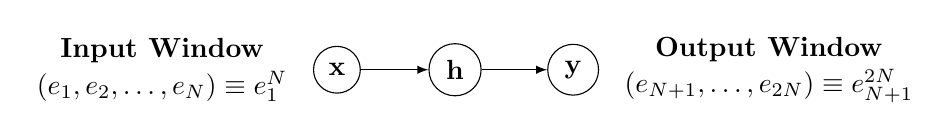
\begin{tikzpicture}[-latex,auto,node distance=1.5cm]
  \tikzstyle{n} = [draw,shape=circle]
  \tikzset{every text node part/.style={align=center}}
  %% nodes for t = 0
  \node (lab-input) {\textbf{Input Window}\\$(e_1,e_2, \ldots, e_N) \equiv e_1^N$};
  \node[n] (x) [right= 0.2cm of lab-input] {$\vect{x}$};
  \node[n] (h) [right of= x] {$\vect{h}$};
  \node[n] (y) [right of= h] {$\vect{y}$};
  \node (lab-output) [right = 0.2cm of y] {\textbf{Output Window}\\$(e_{N+1},
    \ldots, e_{2N}) \equiv e_{N+1}^{2N}$};

  \path (x) edge (h)
        (h) edge (y);

  \end{tikzpicture}
\caption{Windowed feedforward neural network}
\label{fig:windowed-nn}
\end{figure}

Early connectionist approaches to modelling sequential data adapt conventional
feedforward networks to the task by using a finite \emph{windowed} context of
size $N$ and training the network to predict the $N$ events that follow
\cite{todd1989connectionist}. Figure~\ref{fig:windowed-nn} illustrates this
approach.

Observe that, in such an architecture, any common effects between e.g.\ $e_1$
and $e_2$ must be learnt entirely separately from the effects between $e_2$ and
$e_3$, even though there may be a considerable amount of time-invariant
regularity between consecutive events in sequences of interest. Similarly, when
predicting $e_{N+1}^{2N}$, the network will have to learn how to predict each of
these events independently from each other.  

It can be seen that such networks are very \emph{inefficient} sequence learners:
with a large window size, vast amounts of training data and many parameters will
be needed to successfully capture time-invariant effects. Moreover, with a small
window size the network will fail to capture any long-term effects.

One solution to this problem is \emph{parameter sharing}, which is central to
the sequence-learning ability of \emph{recurrent neural networks} (RNNs). To
quote the recent text of Goodfellow et al.\ \cite{Goodfellow-et-al-2016}:
\begin{displayquote}
  ``If we had separate parameters for each value of the time index, we could not
  generalise to sequence lengths not seen during training, nor share statistical
  strength across different sequence lengths and across different positions in
  time.''
\end{displayquote}

For these reasons, we do not consider such feedforward networks in this work,
and instead turn to recurrent networks.

\subsection{Recurrent Neural Networks}

Recurrent neural networks (RNNs), unlike feedforward networks, learn to evolve a
\emph{hidden state} with parameters shared over time. Rumelhart et al.\ first
showed how to train such networks with backpropagation in 1985
\cite{rumelhart1985learning}. RNNs are clearly a natural tool to apply to
sequence learning. However, basic RNNs are known to suffer from the problem of
\emph{vanishing and exploding gradients}. This problem severely hinders the
ability of basic RNNs to learn long-term dependencies: a capacity which is
crucial in our problem domain.

In 1997, the introduction of the \emph{long short-term memory} (LSTM)
architecture by Hochreiter and Schmidhuber \cite{hochreiter1997long} enabled the
construction of RNNs capable of learning dependencies over many more timesteps
than was previously possible. Today, \emph{gated} architectures such as the LSTM
achieve state-of-the-art results in sequence prediction \cite{zaremba2014recurrent}.

\section{Context of the Work}\label{sec:context-of-work}

In the connectionist literature on modelling music, $n$-gram models are often
used as a baseline approach (e.g.\ \cite{boulanger2012modeling}
\cite{liangbachbot}). However, such $n$-gram models are typically only
models of the surface structure, and sophisticated models such as multiple
viewpoint systems are not usually considered.

Similarly, in the literature on multiple viewpoints, performance comparisons to
modern connectionist techniques are rarely drawn. In particular, to the best of
my knowledge, a direct comparison between multiple viewpoint systems and
recurrent networks does not exist. This work therefore draws an interesting, 
novel comparison between two sophisticated yet contrasting approaches.

\section{Structure}

In the following chapter, we introduce the necessary background for the chosen
techniques, as well as justifying the decisions made in order to refine the
proposal ahead of the implementation.  Chapter~\ref{chap:impl} details the
implementation itself. In Chapter~\ref{chap:eval}, the implemented models are
evaluated, with the conclusions presented in Chapter~\ref{chap:conc}.

\chapter{Preparation}

\section{Choice of Techniques}

Despite the strong performance of multiple viewpoint systems (MVSs) when applied
to music, as discussed in Section~\ref{sec:context-of-work}, they are rarely
used as a baseline approach or compared with mainstream machine learning
techniques such as neural networks. The reasons for this, we argue, are
three-fold:
\begin{itemize}
  \item Considerable domain-specific knowledge is required to implement a MVS.
  \item The implementation of a MVS from scratch is reasonably involved for a
    baseline approach.
  \item To the best of my knowledge, no open source framework for implementing
    MVSs exists.
\end{itemize}

Recurrent Neural Networks (RNNs), and LSTM networks in particular, are among the
most successful general sequence-learning models in use at this time. Primarily,
therefore, it is the lack of comparison between these two techniques that
motivates this choice. Secondarily, by choosing to implement a general framework
for multiple viewpoints, it is my intention that an open source project that may
be of use to others can be released.

\section{Starting Point}

Prior to starting this work, I had given a talk on basic $n$-gram approaches to
melody generation using first-order Markov models. This was accompanied by some
code for demonstration purposes. Other than this, I have not done previous
research or implementation in this area. 

I chose to implement the MVS from scratch due to the lack of available
libraries, and based the RNN on an existing library which abstracted away parts
of the implementation that were not of particular interest in this comparison,
such as computing the backwards pass through the network.

Several courses from Part II of the Computer Science Tripos provided background
for the project. The most relevant among these were Information Theory, Machine
Learning, and, supporting the design of the evaluation survey, Human Computer
Interaction. 

\section{Choice of Corpus and Representation}\label{sec:corp-rep}

The chosen corpus was a set of chorale melodies used in the harmonisations of
J.S.\ Bach. The Bach Chorales are a corpus of great interest in the
computational modelling of music: the style is unified, yet with significant
inter-opus variation; it is not too complex, yet not overly simplistic.

Various other musical styles were considered. For example, folk melodies are
often used in this kind of work. These were discarded, since the corpora I
investigated were considered too simplistic to be of interest. Hymn tunes were
also considered; however, the possibility of bias in the evaluation due to
users' familiarity with the samples was of concern.

An internal format for melody based on a widely-used representation in the MVS
literature (e.g.\ \cite{conklin1995viewpoints}) was decided on. Musical time is
quantised with a semiquaver quantum, since this is the smallest note value
encountered in the corpus.

This representation was to be used internally for both the MVS and RNN
implementations. A note $n$ is represented as a tuple $(p,o,d) \in \mathbb{N}^3$
where $p$ is the MIDI pitch of $n$, $o$ is the onset (start time), and $d$ the
duration. A melody is then a list of such tuples. Note that rests are
represented implicitly.

\section{Overview of Music Generation}\label{sec:gen-models}

A system for music generation need not be probabilistic. Techniques such as
genetic algorithms and rule-based systems are capable of generating output
without modelling a probability distribution over the output space. Following
the reasoning of the previous chapter, however, we exclusively consider
probabilistic models. 

\begin{figure}[H]
\centering
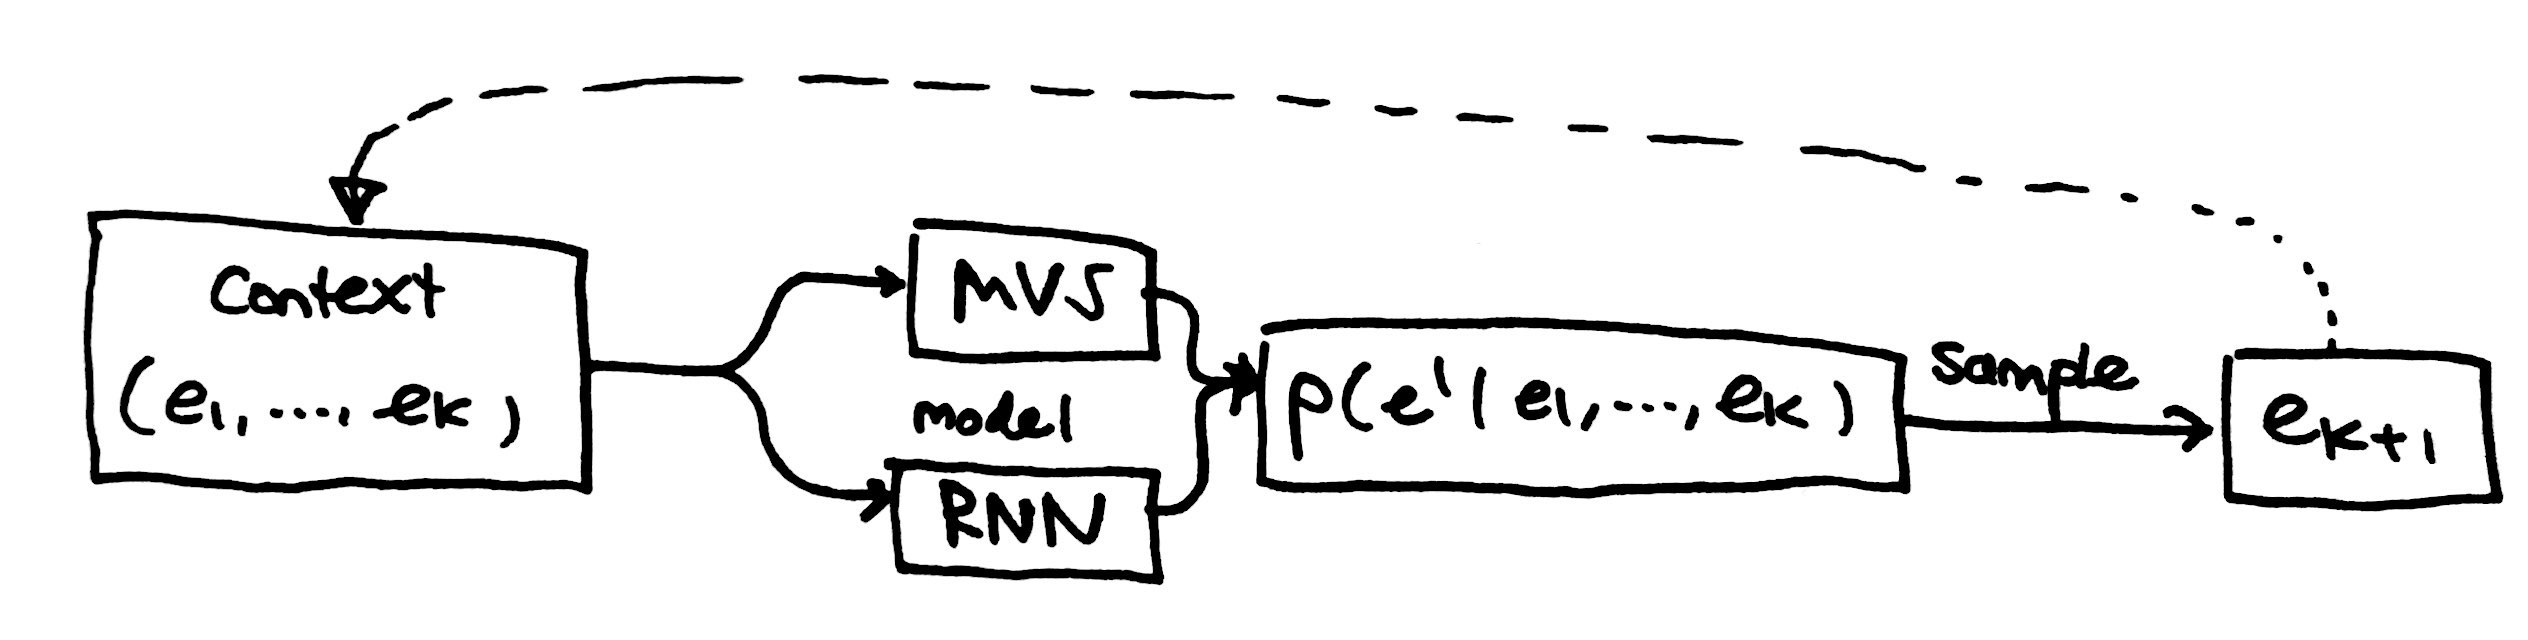
\includegraphics[width=400pt]{figs/high_level_tmp.jpg}
\caption{Overview of probabilistic sequence generation}
\label{fig:seq-gen-overview}
\end{figure}

Any system which models a distribution over data of interest is said to be a
\emph{generative model}. Let $\vect{x} = x_1, \ldots, x_t$ range over sequences
of interest. Then a model which calculates or approximates $p(\vect{x})$ is a
generative model of such sequences.

This distribution is commonly approximated by making an assumption of causality
(\ref{eq:cond-indep}). Both techniques I implement are causal. A high-level
overview of the generation process using such models is given in
Figure~\ref{fig:seq-gen-overview}.
\begin{equation}
  p(\vect{x}) = p(x_t | x_{t-1}, \ldots, x_1) p(x_{t-1} | x_{t-2},
  \ldots, x_1) \cdots p(x_1) \label{eq:cond-indep}
\end{equation} 

An even stronger assumption is the \emph{Markov assumption}, which assumes that
we only need a finite context of length $n$ to be able to predict the next
event, i.e.
\begin{equation}
  p(x_k | x_{k-1}, \ldots, x_1) \approx p(x_k | x_{k-1}, \ldots, x_{k-n}).
  \label{eq:markov-asmptn}
\end{equation} 

In any case, given some generative model approximating $p(\vect{x})$, we can
\emph{sample} from this distribution to obtain an output sequence from the
model. In the case of models that make the assumption of (\ref{eq:cond-indep}),
we can sample by \emph{random walk}, since the probability of the next event
depends only on those that have been generated thus far. At time $t$, for $t =
1$ to $T$, we sample from:
$$ p(x_t | x_{t-1}, \ldots, x_1) $$
and immediately accept the resulting event $x_t$, appending it to our sample.

While random walk sampling is very efficient, running in $\Theta(T)$ time to
generate a sequence of length $T$, it can sometimes generate solutions
$\vect{x}'$ with low $p(\vect{x}')$. Typically, we want to sample sequences that
our model assigns high probabilities. To achieve this, one can 
repeatedly draw samples $\vect{x}'$ by random walk until $p(\vect{x}') > \alpha$
for some threshold $\alpha$: this algorithm is known as \emph{iterative random
walk}.

This project investigates two generative, causal models: multiple viewpoint
systems and recurrent neural networks. To generate a candidate $\vect{x}'$ from
these models, we make use of (iterative) random walk. The next two sections
introduce these models, with a focus on the underlying theory and decisions made
prior to implementation.

\section{Multiple Viewpoint Systems}

In this section, the key theory, algorithms, and data structures underpinning
multiple viewpoint systems are introduced. The formalism is due to Conklin and
Witten \cite{conklin1995viewpoints}. We start by defining some notation which
will be used throughout this section.

\begin{itemize}[itemsep=0mm]
  \item If $\tau$ is a type, then $[\tau]$ is the \emph{syntactic domain} of
    that type: all elements of type $\tau$.   
  \item $S^*$ denotes the set of all sequences drawn from a set $S$.
  \item $e_i^j$ abbreviates the sequence $(e_i,e_{i+1},\ldots,e_{j-1},e_j)$ and
    $()$ the empty sequence.
  \item $s :: e$ denotes the sequence $s$ with event $e$ appended.
  \item $\zeta$ denotes the \emph{event space}, the set of all events that occur
    in sequences of interest. A simple event space for melody might be:
    $$ \zeta = [\mathrm{pitch}] \times [\mathrm{duration}] \times [\mathrm{onset}]. $$
\end{itemize}

\subsection{Context Models}\label{sec:ctx-model-prep}

The central primitive underlying MVSs is the \emph{context model}. In general,
a context model over some type $\tau$ is a data structure storing sequences in
$[\tau]^*$ together with a contextual inference procedure exploiting the Markov
assumption (\ref{eq:markov-asmptn}) to predict distributions over $[\tau]$. 

The underlying data structure is initially specialised from example sequences.
The inference procedure later makes predictions by matching input contexts
against this data structure. The context models I implement are variable-order
Markov models with some maximum history\footnote{ An $n$\textsuperscript{th}
  order Markov chain makes predictions based on $n$ elements of context. For
  notational convenience, and for consistency with the literature, we generally
  refer to the \emph{history} $h = n+1$ of an $n$\textsuperscript{th} order
Markov model.  Such a model stores and models $h$-grams.  } $\hbar$. Such a
model can be thought of as a combination of $\hbar$ Markov models with histories
$1,2,\ldots,\hbar$. 

A known problem with high-order Markov models is their space complexity. A naïve
tabular approach uses $\Theta(|[\tau]|^h)$ space.  In practice, such high-order
models are \emph{sparse}: most $h$-grams are never seen in training. A data
structure which exploits this sparsity is the \emph{suffix tree} or \emph{trie}.
The nodes in a trie are events, each with an associated count, and a path from
the root corresponds uniquely to a particular $h$-gram.
Figure~\ref{fig:dur-trie} illustrates this data structure.

\begin{figure}[H]
\centering
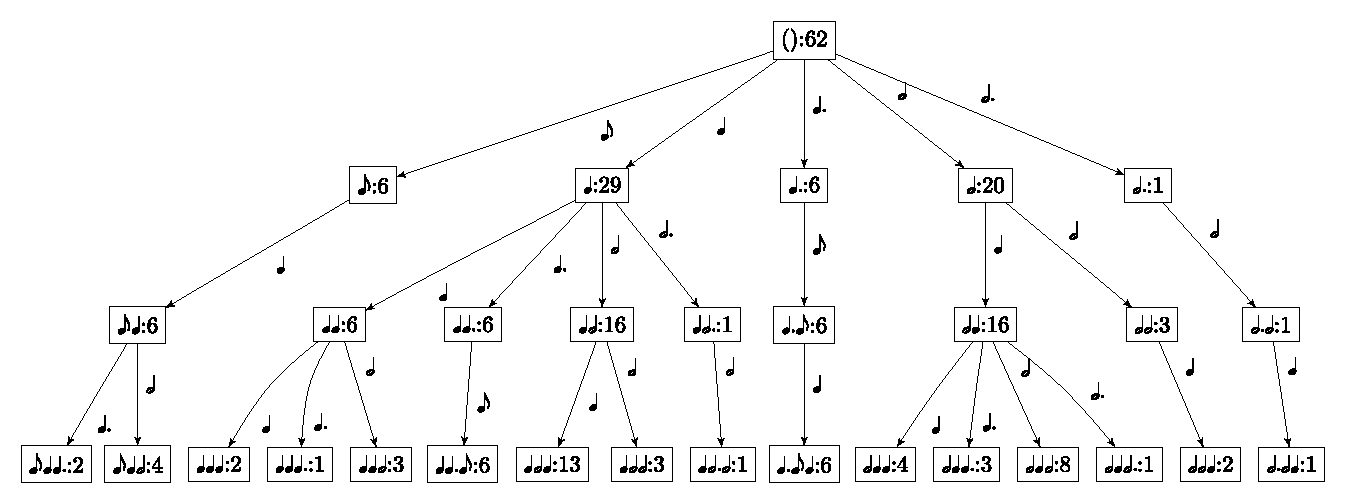
\includegraphics[width=\linewidth]{figs/duration_vp.pdf}
\caption{Trie for context model over musical duration ($\hbar = 3$)}
\label{fig:dur-trie}
\end{figure}

The algorithm for extracting $h$-grams from a training sequence $e_1^k$ works by
passing a sliding window of size $\hbar$ across the input sequence and
generating $h$-grams under this window of size $1$ through $k$. 

\subsubsection{Inference from Context Models}

When performing inference, we want to compute $\mathbb{P}(e' | e_1^k)$ for some
next event $e' \in [\tau]$ and input context $e_1^k \in [\tau]^*$.

An initial attempt might use the maximum likelihood solution to this problem,
which computes the relative frequency of the $h$-gram of interest:
\begin{equation}
  \mathbb{P}(e'|e_1^k) = \frac{ C(e_1^k::e') }{ \sum_{e''} C(e_1^k::e'') }
  \label{eq:ctx-max-like}
\end{equation}
where $C(e_i^j)$ denotes the count associated with $e_i^j$ in the trie, or $0$
if such a node does not exist. Note that all sequences longer than $\hbar$ (and
contexts longer than $\hbar-1$) are implicitly ignored, so $\forall j \in
\mathbb{N}.\ C(e_{k-\hbar-j}^k) = C(e_{k-\hbar+1}^k)$ and
$\mathbb{P}(e'|e_{k-\hbar+1-j}^k) = \mathbb{P}(e'|e_{k-\hbar+2}^k)$.

There are two main problems with this naïve solution. The first is that we want
our models to be \emph{non-exclusive}: all events should be possible, however
improbable. Formally, we require $\forall e' \in [\tau].\ \mathbb{P}(e' | e_1^k)
> 0$. \emph{Exclusive} models have limited scope for creativity, and moreover,
from a practical standpoint, evaluation metrics such as \emph{cross-entropy}
calculate log-probabilities: we therefore need to avoid zero probabilities. This
naïve approach, however, fails to guarantee non-exclusivity.

The second problem with this solution is that it cannot handle \emph{novel
contexts}. Suppose we have not seen the context $e_1^k$. Then, clearly, the
denominator of (\ref{eq:ctx-max-like}) will be zero, which is equally
problematic.

I chose to implement an algorithm which attends to both of these issues:
\emph{prediction by partial match} (PPM) \cite{cleary1984ppm}. The central idea
behind PPM is that, instead of distributing the probability mass entirely among
the exact matches, as per (\ref{eq:ctx-max-like}), we instead reserve some
amount of the probability mass for as-yet unseen symbols. This reserved
probability mass is known as the \emph{escape probability}. The escape
probability is then distributed recursively among a lower-order model. In this
sense, PPM belongs to the more general class of \emph{backoff smoothing}
algorithms.

Backoff smoothing algorithms are typically formulated recursively, as per
(\ref{eq:ppm-general}).
\begin{equation}\label{eq:ppm-general}
  \mathbb{P}(e' | e_1^k) = \begin{cases}
  \alpha(e'|e_1^k) & C(e' | e_1^k) > 0 \\
\gamma(e_1^k) \cdot \mathbb{P}(e' | e_{(k - \hbar) + 2}^k) & \text{otherwise}
\end{cases} 
\end{equation} 

The choice of escape probability $\gamma(\cdot)$ is known as the \emph{escape
method}: established methods include A, B, C, D, and AX
\cite{pearce2004improved}. PPM A, which we choose for simplicity, takes:
\begin{align}
  \label{eq:ppm-a-alpha}
  \alpha(e' | e_1^k) &= \frac{ C(e' | e_1^k) }{ 1 + \sum_{e''} C(e'' | e_1^k) }
  \\
  \gamma(e_1^k) &= \frac{ 1 }{ 1 + \sum_{e'} C(e' | e_1^k) }
  \label{eq:ppm-a-gamma}
\end{align}

It is clear from this formulation that all events are assigned some non-zero
probability, meaning that PPM gives rise to non-exclusive models. For any unseen
context, PPM deterministically backs off to the next lowest-order model. If no
match is found for any model, the recursion bottoms out with a uniform
distribution. 

This recursive formulation can be somewhat misleading, as the notation implies
that (\ref{eq:ppm-general}) gives rise to properly normalised probability
distributions. This is in fact not the case. 

\begin{figure}[H]
\centering
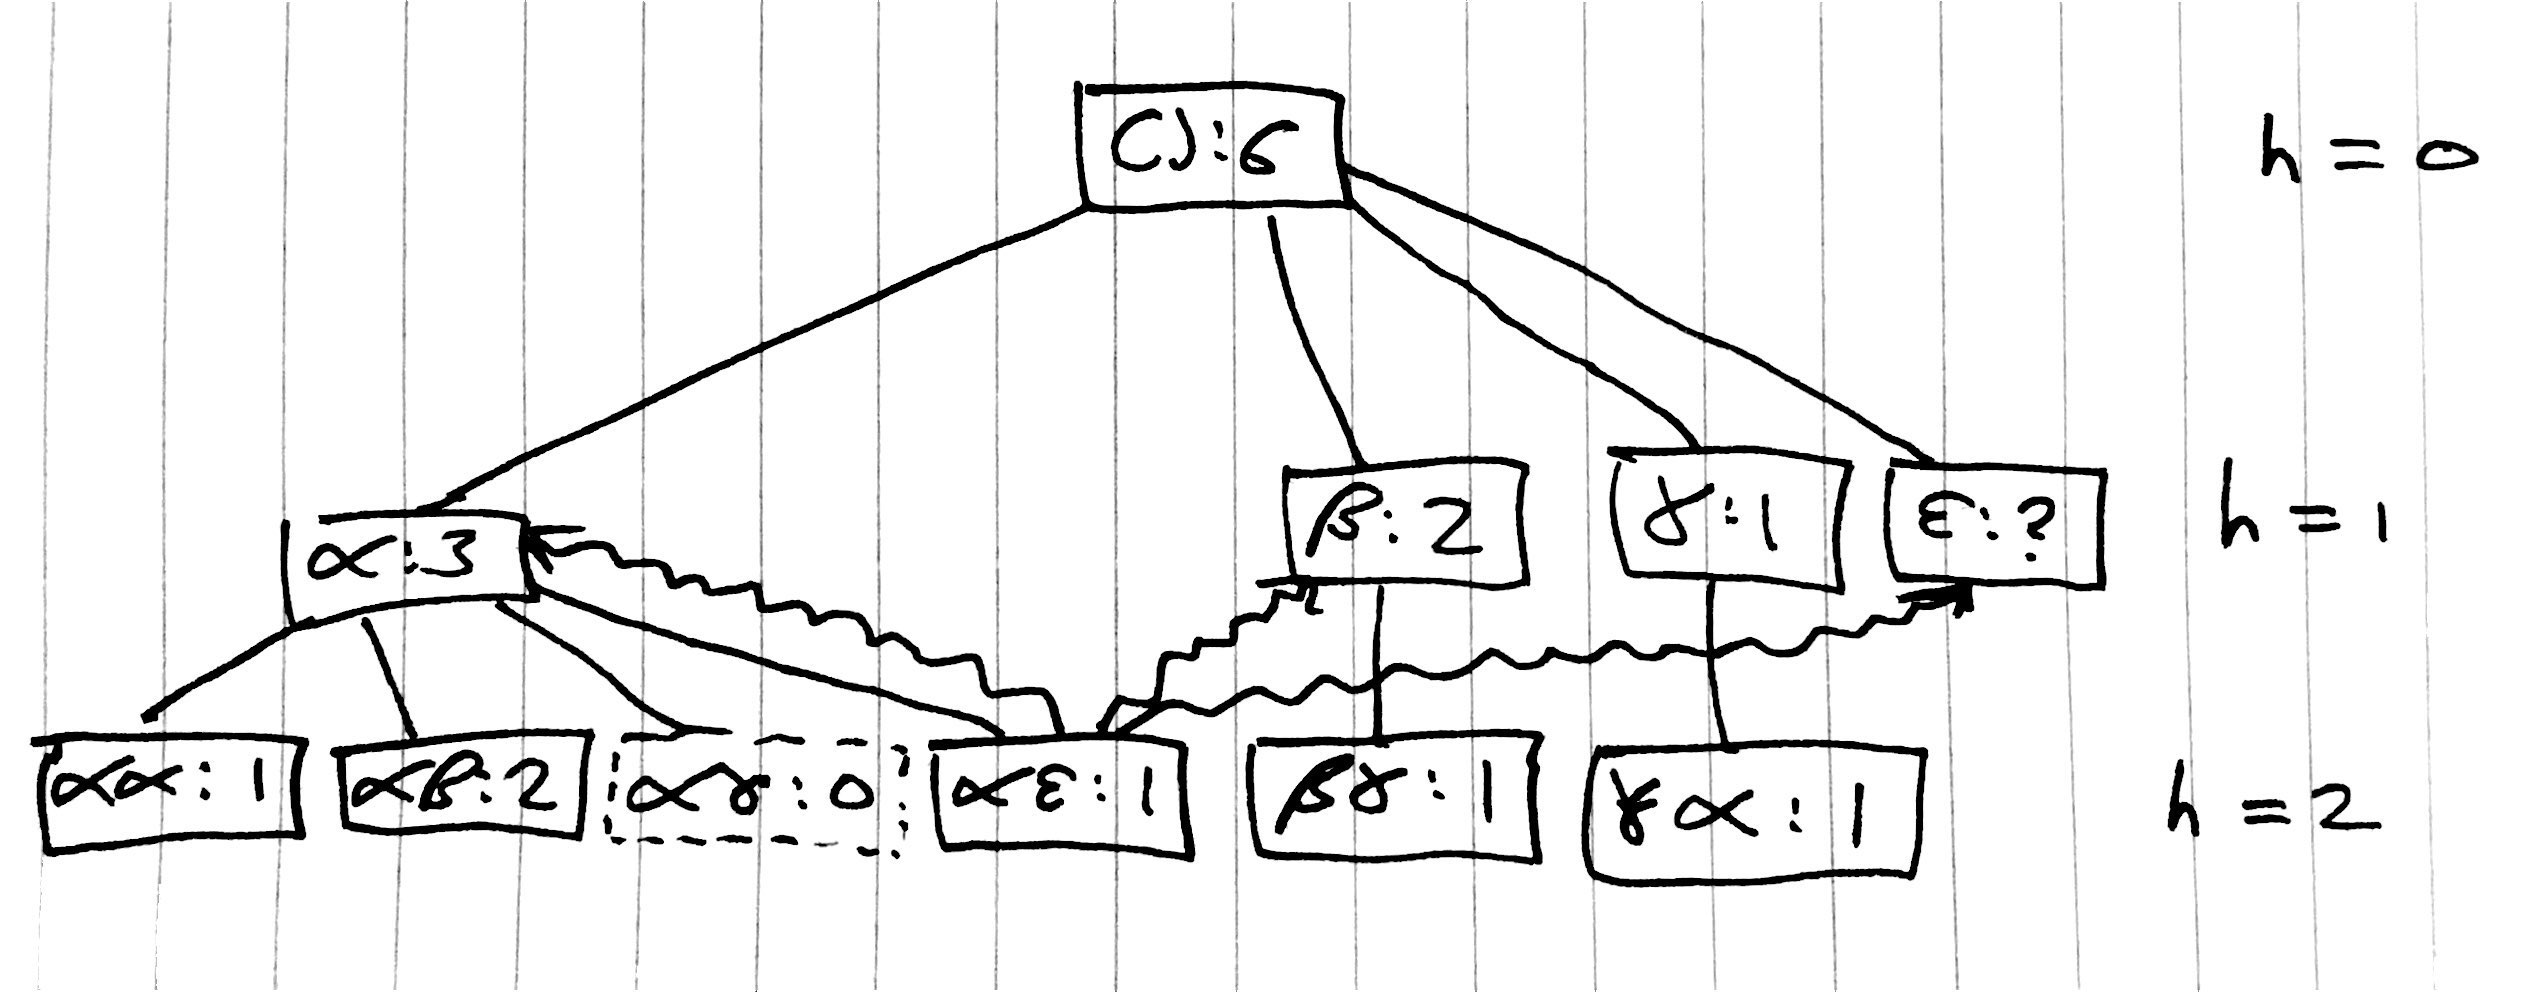
\includegraphics[width=400pt]{figs/problematic_trie_tmp.jpg}
\caption{Trie demonstrating lack of normalisation in standard PPM.}
\label{fig:bad-ppm-trie}
\end{figure}

To see this, consider performing PPM with $\hbar = 2$ over an alphabet $\Sigma =
\set{\alpha,\beta,\gamma}$, and suppose we have seen the training sequence
$(\alpha,\beta,\gamma,\alpha,\alpha,\beta)$.  Figure~\ref{fig:bad-ppm-trie}
illustrates the situation, and includes virtual $\epsilon$-nodes to represent
the escape mass.

The first problem is the escape node at layer $h = 1$. According to
(\ref{eq:ppm-a-gamma}) it should have an effective count of $1$. However, this
yields:
\begin{align}
  \sum_{e \in \Sigma} \mathbb{P}(e) = \frac{3}{7} + \frac{2}{7} + \frac{1}{7} =
\frac{6}{7} \neq 1. 
\end{align} 
The observation to make here is that if \emph{all} symbols in our alphabet have
a non-zero count for any given context, then the escape probability is
redundant. Suppose, then, we set the effective count of this $\epsilon$-node to
zero. Consider the distribution $\mathbb{P}(e|\alpha)$. We can trivially compute
$\mathbb{P}(\alpha|\alpha) = 1/4$ and $\mathbb{P}(\beta|\alpha) = 1/2$, and for
$\gamma$ we escape to find $\mathbb{P}(\gamma|\alpha) = 1/4 \cdot
\mathbb{P}(\gamma)$. However, $\mathbb{P}(\gamma) < 1$, so
$\mathbb{P}(e|\alpha)$ is not normalised. The problem here is that the escape
mass for the node labelled $\alpha\epsilon$ is distributed among all the symbols
at layer $h = 1$ in the trie, when actually we can only ever escape to $\gamma$.

There are two typical solutions for this lack of normalisation in PPM: in
earlier work, authors often compute an improper distribution and later normalise
it (e.g.\ \cite{conklin1990prediction}). A better-performing and less wasteful
solution which reasons about the possible escape paths is known as PPM with
\emph{exclusion} \cite{pearce2004improved}. I chose to implement exclusion for
the context models in this work.

\subsection{Viewpoints}\label{sec:mvs-formalism}

One possible approach to modelling music would be to form a context model over
the entire event space $\zeta$.  Recall $\zeta = [\tau_1] \times [\tau_2] \times
\cdots \times [\tau_n]$ is the cartesian product of many domains. Aside from
being computationally expensive, this approach is severely limited in its
predictive power, since it requires an \emph{exact match} of the musical context
to make useful predictions: the system cannot \emph{generalise} to unseen
contexts.  Figure~\ref{fig:generalise} illustrates this problem.

\begin{figure}[H]
\centering
\input{figs/generalise.pdf_tex}
\caption{Melodic fragments illustrating importance of generalisation}
\label{fig:generalise}
\end{figure}

An obvious approach to achieve generalisation would be to model some or all of
the $\tau_i$ \emph{independently}. While there is some correlation between e.g.\
pitch and duration, much of the rhythmic regularity in music is
pitch-independent. Hence, it might be effective to model duration independently
of other attributes. Similarly, Fragment (b) of Figure~\ref{fig:generalise}
motivates modelling \emph{pitch} independently of duration.

Furthermore, complex languages such as music can be viewed using many abstract
interpretations. A simple example is the \emph{melodic contour} with domain
$\set{-1,0,1}$ which indicates whether a melody is falling, stationary, or
rising. An immediately useful example is the \emph{melodic interval}, which
exploits the fact that intervalic patterns in most music capture regularity
\emph{invariant} to the absolute pitch. Fragment (c) of
Figure~\ref{fig:generalise} motivates this interpretation. Modelling regularity
in such abstract domains and transforming the predictions back into predictions
over the concrete $\tau_i$ might therefore enable further generalisation.

\emph{Viewpoints} allow us to model music with great flexibility: we can model
the individual $\tau_i$, as well as abstract interpretations and combinations
thereof. We now proceed to set up the formalism of multiple viewpoints.

First, allow $\tau$ to range over types other than just the \emph{basic types}
that make up the component types of $\zeta$. We call these non-surface types
\emph{derived types}: the abstract interpretations of the surface $\tau_i$. 

\textbf{Definition}. A \emph{viewpoint} modelling a type $\tau$ is:
\begin{enumerate}[label=\arabic*., itemsep=0mm]
  \item a partial function $\Psi_\tau : \zeta^* \rightharpoonup [\tau]$,
    together with
  \item a context model of sequences in $[\tau]^*$.
\end{enumerate}

The function $\Psi_\tau$ for a type $\tau$ is known as the \emph{projection}
function for $\tau$: it projects out the last element of type $\tau$ from some
surface event stream $e_1^k \in \zeta^*$, if such an element exists. Note that,
for convenience, we frequently refer to viewpoints simply by the type they
model. 

Viewpoints, as we have defined them, can clearly model individual surface and
derived types independently. While this is useful, we still need to be able to
model the correlation between basic attributes.

\textbf{Definition}. A \emph{product type} $\tau_1 \otimes \cdots \otimes
\tau_n$ between $n$ types $\tau_1, \ldots, \tau_n$ is itself a type $\tau$ with
$[\tau] = [\tau_1] \times \cdots \times [\tau_n]$. 

For a product type $\tau = \tau_1 \otimes \cdots \otimes \tau_n$:
$$ \Psi_\tau(e_1^k) \triangleq
\begin{cases}
  \langle\Psi_{\tau_1}(e_1^k), \ldots, \Psi_{\tau_n}(e_1^k)\rangle & \forall i
  \in \set{1,\ldots,n}.\
  \Psi_{\tau_i}(e_1^k)\downarrow \\
  \bot & \text{otherwise.}
\end{cases}
$$

Viewpoints over product types are known as \emph{linked viewpoints}. 

Note that \emph{threaded viewpoints}, those defined only at certain fixed
intervals in a sequence, are considered out of scope for this work.

In order to train a viewpoint of type $\tau$, we need to provide the
underlying context model with sequences in $[\tau]^*$. To obtain such sequences
from surface events, we simply iterate the projection function $\Psi_\tau$ to
give a function $\Phi_\tau : \zeta^* \rightarrow [\tau]^*$ which we call the
\emph{lifting} function, defined as follows:
\begin{align*}
  \Phi_\tau(()) &\triangleq () \\
  \Phi_\tau(e_1^k) &\triangleq \begin{cases}
    \Phi_\tau(e_1^{k-1})::\Psi_\tau(e_1^k) & \Psi_\tau(e_1^k)\downarrow \\
    \Phi_\tau(e_1^{k-1}) & \text{otherwise.}
  \end{cases}
\end{align*}

In practice, we shall see that it is typically easier to implement $\Phi_\tau$
directly. However, formally, it is cleaner to specify $\Psi_\tau$ to define a
particular viewpoint.

Now consider a viewpoint over a type $\tau$ derived from some basic type
$\tau'$. This viewpoint will predict distributions over the abstract type
$\tau$, but we really need a distribution over the concrete $\tau'$. 

The process of transforming a distribution from the abstract domain to the
concrete is given limited treatment in the literature. Whorley
\cite{whorley2013phd} notes that this is effectively ``using the partial
function $\Psi_\tau$ in reverse on each of the viewpoint elements.'' We argue
that the surface context is also needed to perform this task, and will refer to
this process as \emph{reification}, specified by a partial function $\rho :
\zeta^* \times \mathrm{dist}(\tau) \rightharpoonup \mathrm{dist}(\tau')$, where
$\mathrm{dist}(\tau)$ denotes the set of probability distributions over a type
$\tau$. This will be discussed further in Chapter~\ref{chap:impl}.

\subsection{Combining Viewpoint Predictions}\label{sec:vp-comb}

Recall that, given some musical context $e_1^k \in \zeta^*$, the goal is to
predict the next event $e_{k+1} \in \zeta$ where $\zeta = [\tau_1] \times \cdots
\times [\tau_n]$.  A collection of viewpoints that performs this task is known
as a \emph{multiple viewpoint system} (MVS). 

A MVS decomposes this task by predicting $e_{k+1}$ componentwise. Consider all
viewpoints capable of predicting some basic type $\tau_i$. At each timestep,
given the context $e_1^k$, $N$ of these will \emph{activate}, meaning they
predict a distribution for $\tau_i$. This section concerns methods for the
combination of $N$ such distributions to form an overall prediction. In
particular, we consider \emph{weighted} schemes as these are widely used in the
literature and are known to perform better than unweighted schemes
\cite{pearce2004combining}.

The premise of weighted schemes for viewpoint combination is that predictions
with lower uncertainty should be given higher weights.  Since the Shannon
entropy of a viewpoint's distribution is a metric of overall uncertainty, we use
weights that are monotonically non-increasing as a function of distribution
entropy.

Suppose we have $N$ distributions over a type $\tau$. Suppose further that there
is some canonical ordering of $[\tau]$, such that we can pick out the
$j$\textsuperscript{th} member. Now, let $p_i(j)$ denote the probability
assigned to $j$\textsuperscript{th} element by the $i$\textsuperscript{th} of the
$N$ distributions. We want to combine these predictions to produce some overall
distribution with
probabilities $p(j)$.

A general weighted arithmetic scheme combines the predictions as follows:
$$
  p(j) = \frac{ \sum_{i = 1}^N w_i p_i(j) }{ \sum_{i = 1}^N w_i }.
$$

The Shannon entropy of the $i$\textsuperscript{th} distribution is given by:
$$ H(i) = - \sum_{j = 1}^{|[\tau]|} p_i(j) \log_2 p_i(j) $$
with maximum value $H_{\mathrm{max}} = \log_2{ |[\tau]| }$. Now define the
\emph{normalised entropy} $\hat{H}(i)$ as:
$$ \hat{H}(i) \triangleq \begin{cases}
  H(i)/H_{\mathrm{max}} & H_{\mathrm{max}} > 0 \\
  1 & \text{otherwise.}
\end{cases} $$

Finally, to favour distributions with lower $\hat{H}$ (lower uncertainty), we
introduce an exponential bias $b \in \mathbb{R}_0^+$: $$ w_i = \hat{H}(i)^{-b}.
$$

Note that we do not restrict $b$ to integer values, as is usually done in the
literature \cite{whorley2013phd}. 

Pearce \cite{pearce2004improved} introduces a new method for distribution
combination which outperforms arithmetic schemes, a \emph{weighted geometric
mean}:
$$ p(j) = \frac{1}{Z} \left( \prod_{i = 1}^N p_i(j)^{w_i} \right)^{ \frac{1}{
\sum_{i = 1}^N w_i }} $$
where $Z$ is a normalisation constant, and the $w_i$ are calculated as before.

Figure~\ref{fig:dist-comb-plot} shows the effect of using these two schemes on
some example distributions. It can be seen that low-probability predictions from
have considerably more bearing with the geometric scheme.

Note also that when combining distributions $C$ and $D$, since $D$ has much
lower entropy (greater certainty), it has considerably more effect on the
overall result under both schemes.

I chose to first implement the arithmetic scheme as a baseline approach and
later implement the geometric scheme.

\begin{figure}[H]
\centering
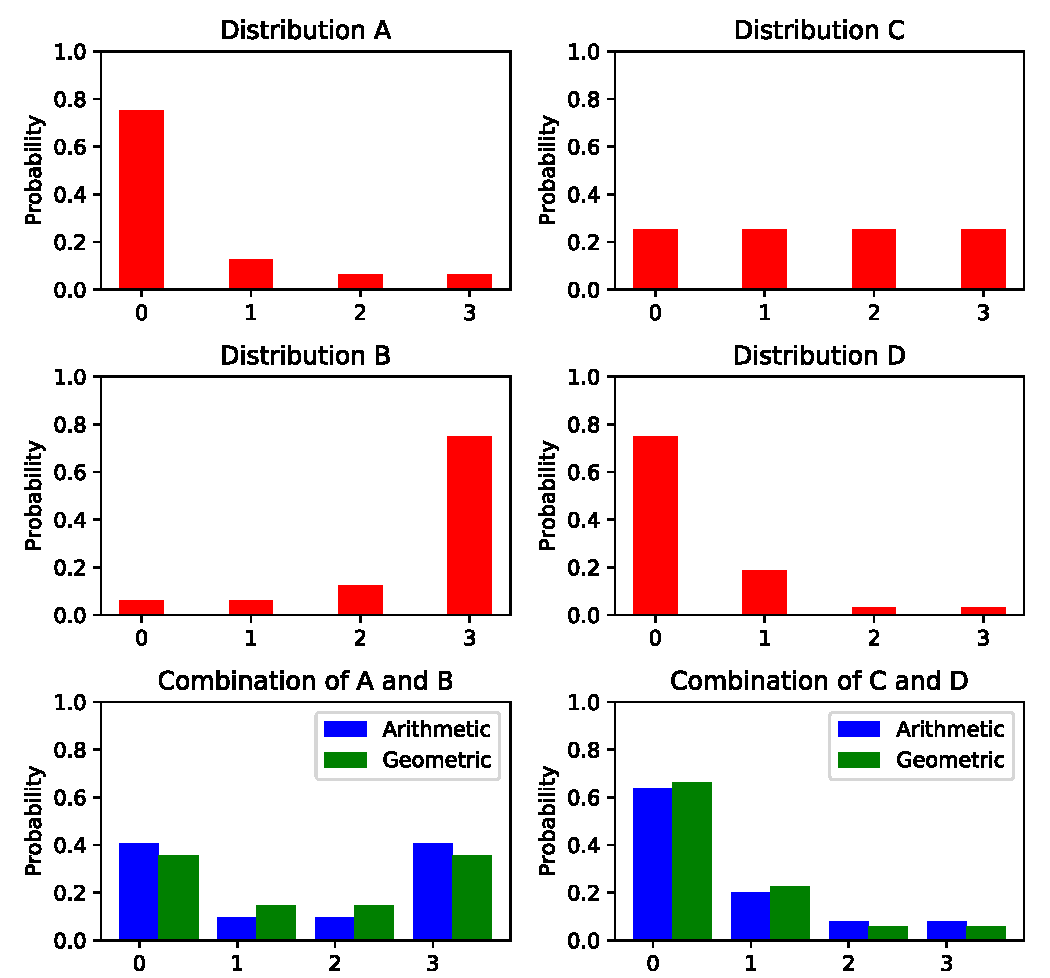
\includegraphics[width=400pt]{figs/dist_comb.pdf}
\caption{Plots illustrating distribution combination schemes ($b = 2$)}
\label{fig:dist-comb-plot}
\end{figure}

\subsection{MVS Architecture}\label{sec:mvs-arch}

\begin{figure}[H]
\centering
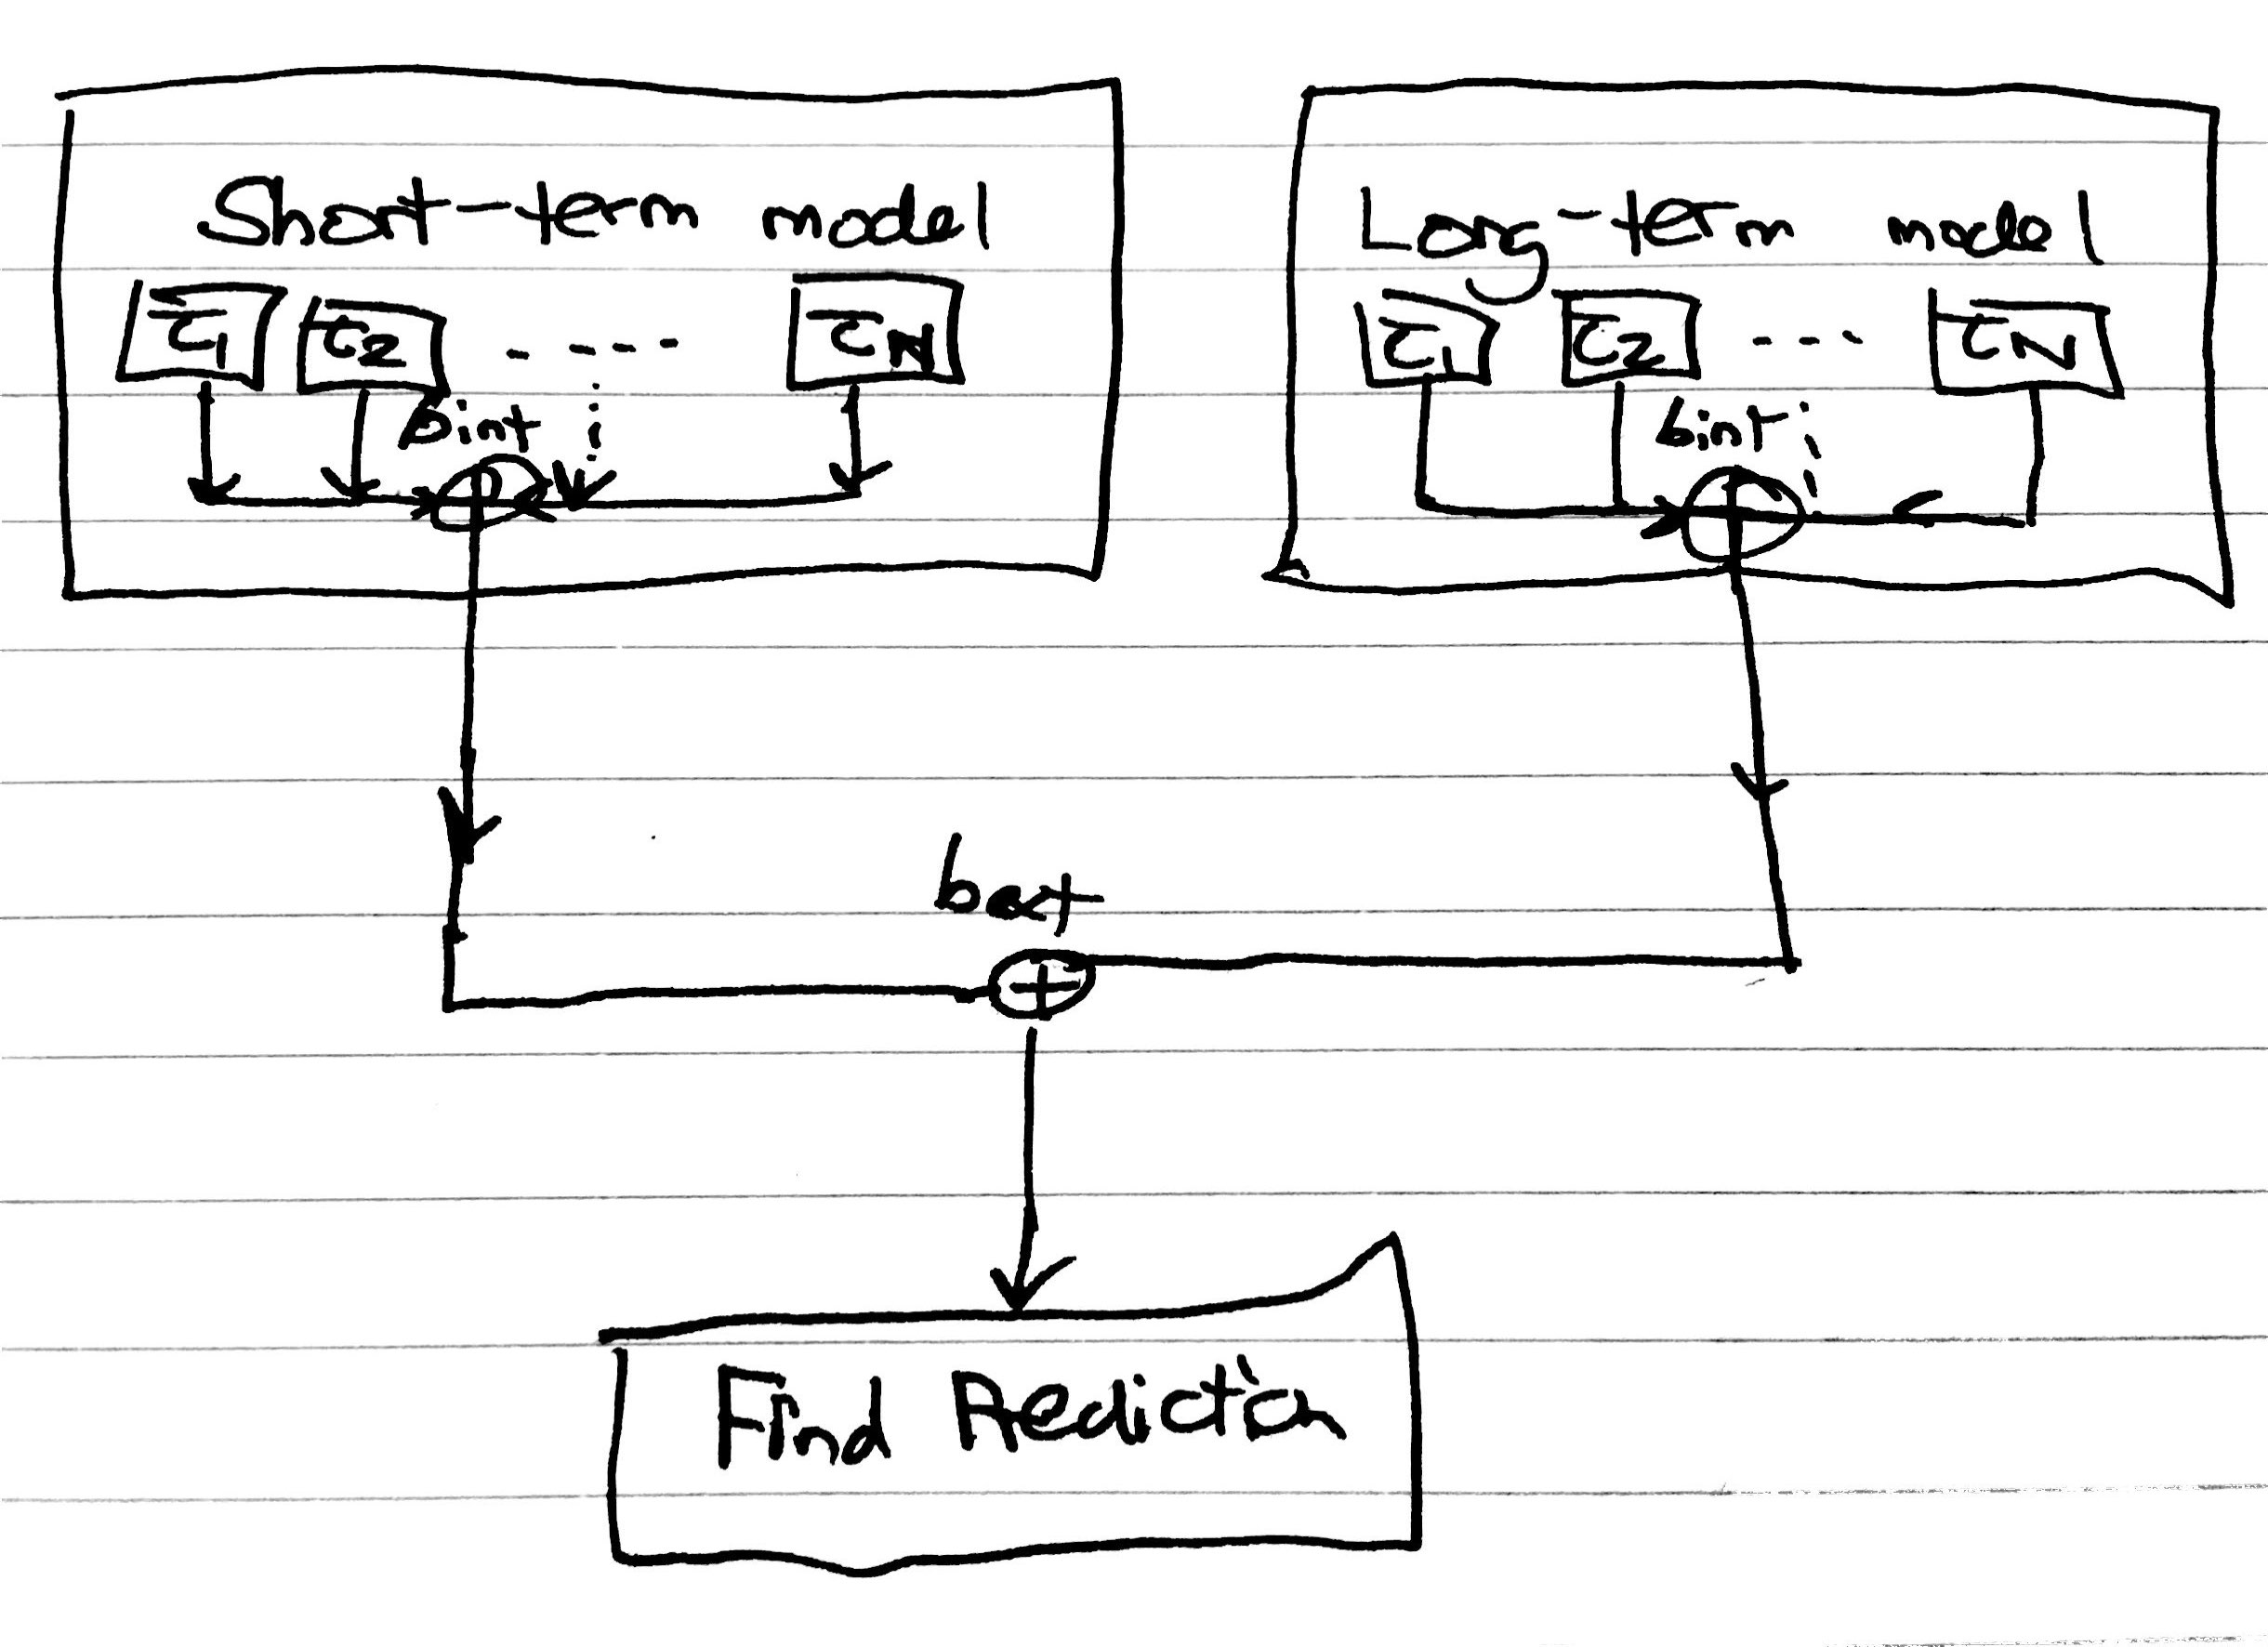
\includegraphics[width=250pt]{figs/mvs_arch_tmp.jpg}
\caption{Typical MVS architecture}
\label{fig:mvs-arch}
\end{figure}

For successful sequence prediction, it is necessary to capture both
intra-sequence and inter-sequence regularity: that is, the \emph{short-term}
effects \emph{local} to a particular sequence, and the \emph{long-term} effects
common through the entire corpus.  This is especially true of music, and indeed
the chorales, where entire melodic fragments are often re-used within a given
chorale melody.

In a MVS, this is achieved explicitly with separate \emph{long-term} and
\emph{short-term} models. The long-term model (LTM) is trained on the entire
corpus, and the short-term model (STM) just on the sequence being predicted or
generated. Figure~\ref{fig:mvs-arch} illustrates this architecture: viewpoint
combination is indicated by $\oplus$, and is performed as per
Section~\ref{sec:vp-comb}.

In order to control the number of hyperparameters, the following architectural
constraints are enforced:
\begin{itemize}
  \item The same set of viewpoints $\set{\tau_1, \ldots, \tau_N}$ is used in both
    the LTM and STM. 
  \item The viewpoints in the LTM all have order bound $h_l$. Similarly, those
    in the STM have order bound $h_s$.
  \item Viewpoint combination within the LTM and STM is performed using the same
    bias parameter $b_{\mathrm{int}}$ and the combination of their predictions
    using a separate bias parameter $b_{\mathrm{ext}}$.
\end{itemize}

\vspace{8mm}

We now turn to our second technique of choice: recurrent neural networks.

\section{Recurrent Neural Networks}\label{sec:rnn-intro}

\begin{figure}[H]
\centering
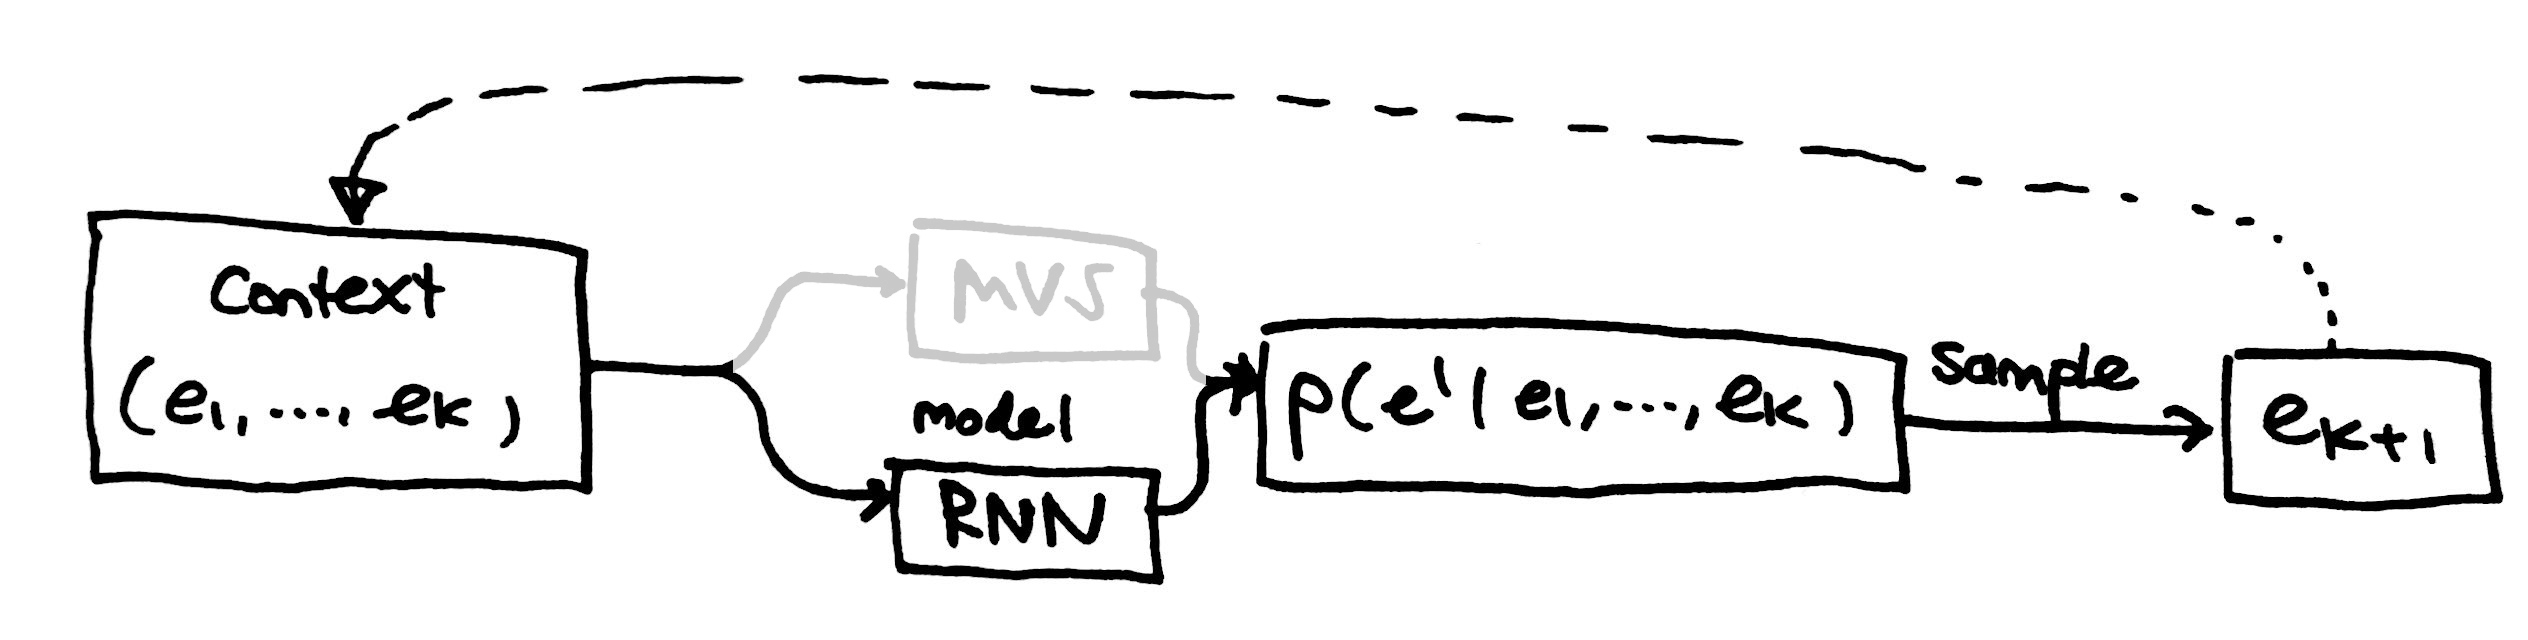
\includegraphics[width=400pt]{figs/high_level_rnn_tmp.jpg}
\caption{Overview of music generation using RNN}
\label{fig:rnn-gen-overview}
\end{figure}

RNNs can be formulated as a dynamical system with a state evolving over time.
Given an initial state $\vect{h}_0$ and input data $\vect{x}_t \in
\mathbb{R}^m$, the hidden state $\vect{h}_t \in \mathbb{R}^n$ evolves as per
(\ref{eq:dyn-sys}) for $t \in \mathbb{N}$.
\begin{equation}
  \vect{h}_t = f(\vect{h}_{t-1}, \vect{x}_t; \vect{\theta})
  \label{eq:dyn-sys}
\end{equation} 

The output $\vect{o}_t$ is typically a function of $\vect{h}_t$. The key
observation to make from (\ref{eq:dyn-sys}) is that the same parameters
$\vect{\theta}$ are used in each application of $f$. 

In a basic RNN, the choice of $f$ is a simple neural network unit: a
nonlinearity (such as $\tanh$ or the logistic sigmoid) applied to an affine
transformation \cite{zaremba2014recurrent}. Using
$[\vect{u},\vect{v}] \in \mathbb{R}^{m+n}$ to denote the concatenation of
vectors $\vect{u} \in \mathbb{R}^m, \vect{v} \in \mathbb{R}^n$: 
$$f(\vect{h}_{t-1}, \vect{x}_t) = \sigma(\vect{W}[\vect{h}_{t-1}, 
\vect{x}_t] + \vect{b})$$ 
where $\vect{W} \in \mathbb{R}^{(m+n) \times n}$, and $\vect{b} \in
\mathbb{R}^n$. 

The next section explains how we can train recurrent networks, and then explores
some of the problems due to this simple choice of $f$.

\subsection{Training Recurrent Networks}\label{sec:rnn-train}

The algorithm used for training a RNN, known as \emph{backpropagation through
time} (BPTT), calculates the derivative of the cost function with respect to the
weights in our network \emph{at each timestep}. Since the parameters are shared
across time, we sum the gradient contributions from each timestep and update the
weights accordingly by gradient descent.

\begin{figure}[H]
\centering
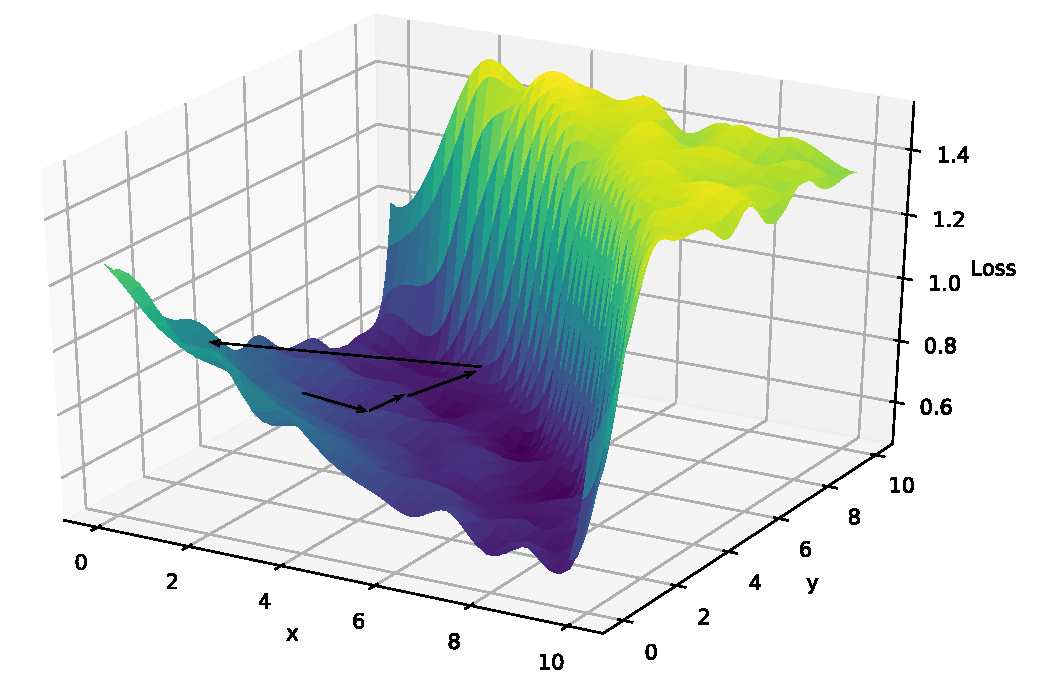
\includegraphics[width=400pt]{figs/exploding_gradients.pdf}
\caption{Optimisation damage due to exploding gradients}
\label{fig:exploding-grad}
\end{figure}

The repeated composition of the function $f$ in such a network can exhibit
highly nonlinear behaviour. While this can be desirable, granting the network
considerable expressivity, training such networks can be problematic. 

One such problem in deep networks is known as the \emph{exploding gradient
problem}, where the high-dimensional surface of our loss function with respect
to the weights exhibits sharp ``cliffs'' where the gradient is very large
\cite{Goodfellow-et-al-2016}. The negative effects of this problem on training,
illustrated in Figure~\ref{fig:exploding-grad}, can largely be mitigated by
\emph{clipping} the the gradients to some maximum norm during training.

\subsubsection{Long-term dependencies}

A more insidious problem with basic recurrent networks is the \emph{vanishing
gradient problem}. This is caused not only by the network being very deep, but
in particular by the repeated application of $f$ with the same parameters at
each timestep.

Here, we follow Goodfellow et al.\ \cite{Goodfellow-et-al-2016} and refer to
Hochreiter et al.\ \cite{hochreiter1997long} for a deeper treatment.
This argument makes several simplifying assumptions, but clearly illustrates how
the problem might arise.

Suppose we simplify the function composition in a neural network to simply apply
matrix multiplication (no inputs, biases, or nonlinearities). The
recurrence relation: 
$$ \vect{h}_t = \vect{W}^\top \vect{h}_{t-1} $$ 
describes the evolution of such a network. A straightforward induction shows:
$$ \vect{h}_t = (\vect{W}^t)^\top\vect{h}_0 $$
and, supposing that $\vect{W}$ has an eigendecomposition of the form:
$$ \vect{W} = \vect{Q}\vect{\Lambda}\vect{Q}^\top $$
with orthogonal $\vect{Q}$ (i.e.\ $\vect{Q}\vect{Q}^\top = \vect{Q}^\top\vect{Q}
= \vect{I}$), the recurrence can be further simplified to:
$$ \vect{h}_t = (\vect{Q}^\top \vect{\Lambda}^t \vect{Q}) \vect{h}_0. $$
As $t \rightarrow \infty$, any eigenvalues with less than unit magnitude will
vanish, and those with magnitude greater than unity will explode. The problem of
vanishing and exploding gradients comes from the fact that gradients through the
graph of such a network are \emph{also} scaled according to $\vect{\Lambda}^t$
\cite{Goodfellow-et-al-2016}.

Modelling complex languages such as music requires learning long-term
dependencies in sequences. However, if the gradient vanishes in this manner as
we look further back in time, then gradient descent will experience an
exponential slow-up in learning such dependencies. For this reason, learning
long-term dependencies with basic RNNs is considered intractable.

\subsection{Long Short-Term Memory}\label{sec:lstm-prep}

In 1997, Hochreiter et al.\ discovered a radically different RNN architecture
known as \emph{long short-term memory} (LSTM) \cite{hochreiter1997long}. The
architecture is based on a simple fundamental idea which is used to achieve
constant gradient flow through time, enabling LSTM networks to learn
dependencies over many timesteps. The idea is to maintain additional state known
as the \emph{cell state} which flows through the network with only minor
\emph{linear}, \emph{pointwise} interactions.

In a deep recurrent network, information is not only processed horizontally
through time, but also vertically through $L$ hidden layers ($L > 1$). We use a
homogeneous state representation with all states in $\mathbb{R}^n$.

Let subscripts denote timesteps and superscripts denote layers so that
$\vect{h}_t^l \in \mathbb{R}^n$ denotes the state at time $t$ in layer $l$. To
represent events $x_t$ drawn from an alphabet $\Sigma$ as vectors in
$\mathbb{R}^n$, we use an embedding $E : \Sigma \rightarrow \mathbb{R}^n$ which
is either pre-trained or learned together with the weights for the network. Let
$\vect{h}_t^0 = E(x_t)$ denote the input vector at time $t$ and take
$\vect{h}_t^L$ as the output vector at time $t$.

A deep RNN is specified by a transition function from previous to current
states:
$$ \delta : \vect{h}_t^{l-1}, \vect{h}_{t-1}^l \rightarrow \vect{h}_t^l $$
so a basic RNN as per Section~\ref{sec:rnn-intro} can be specified as:
$$ \delta(\vect{h}_{t-1}^l, \vect{h}_t^{l-1}) = f(\vect{W}^l_x [\vect{h}_{t-1}^l,
\vect{h}_t^{l-1}] + \vect{b}^l_x) $$
where $\vect{W}^l_x \in \mathbb{R}^{2n \times n}$, $\vect{b}^l_x \in
\mathbb{R}^n$, and $f \in \set{ \sigma, \mathrm{tanh} }$ is a nonlinearity.

Typically, in sequence prediction, the output state $\vect{h}_t^L$ at time $t$
is fed into a densely connected layer to obtain an output $\vect{o}_t \in
\mathbb{R}^{|\Sigma|}$:
$$ \vect{o_t} = \vect{W}_y \vect{h}_t^L + \vect{b}_y $$
where $\vect{W}_y \in \mathbb{R}^{n \times |\Sigma|}$ and $\vect{b}_y \in
\mathbb{R}^{|\Sigma|}$. 

Treating $\vect{o}_t$ as log-probabilities, we obtain a probability distribution
over output symbols $y_t \in \Sigma$ with a softmax activation on this layer:
$$ p(y_t) = \mathrm{softmax}(\vect{o}_t) $$
where for a vector $\vect{z} \in \mathbb{R}^n$, $\mathrm{softmax}(\vect{z})$ is
given by:
$$ \mathrm{softmax}(\vect{z})_i = \frac{ e^{z_i} }{ \sum_{j = 1}^n e^{z_j} }. $$

Figure~\ref{fig:deep-rnn-arch} illustrates the general architecture of a deep
RNN. The merging of arrows denotes \emph{vector concatenation}. The units
$A_t^l$ are known as \emph{cells}, specified by the transition function
$\delta$.  Note that weight sharing occurs across time, but not between layers.
The initial states $\vect{h}_{\mathrm{init}}^l$ can be set to $\vect{0}$ or
initialised randomly.

\begin{figure}[H]
\centering
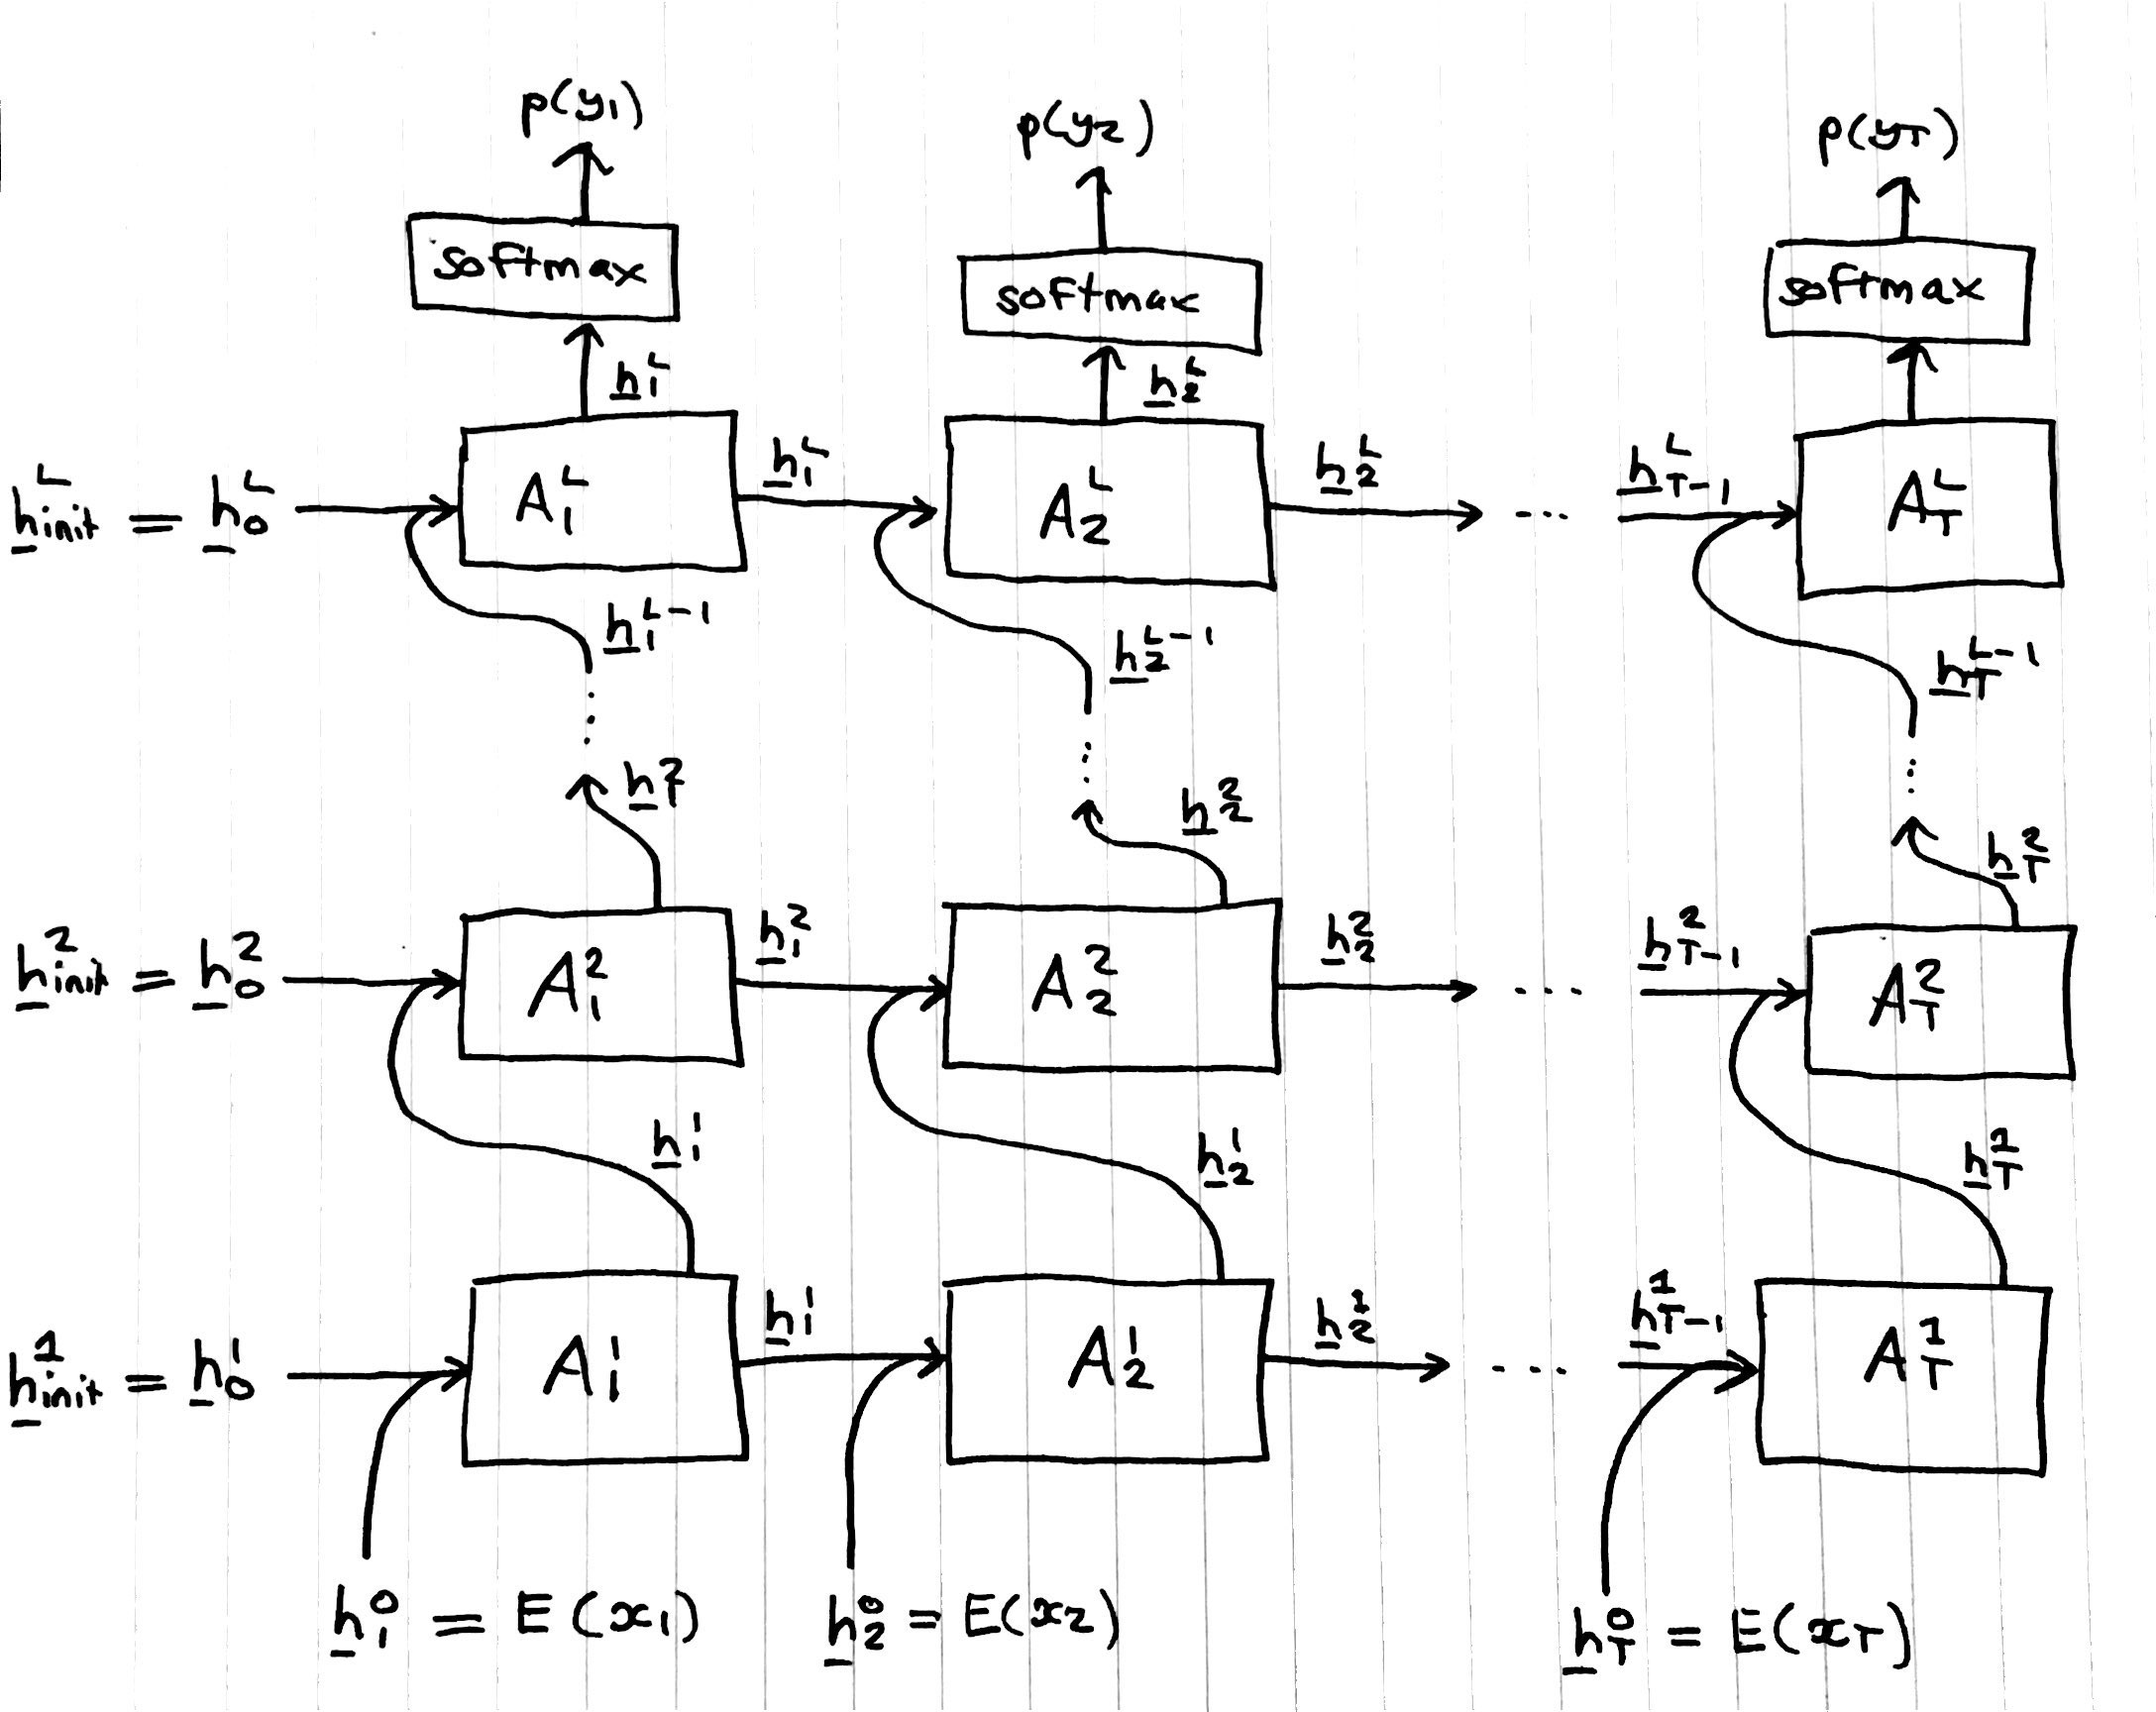
\includegraphics[width=400pt]{figs/deep_rnn_tmp.jpg}
\caption{Flow of information in deep RNN}
\label{fig:deep-rnn-arch}
\end{figure}

Since LSTMs maintain an additional cell state $\vect{c}_t^l$, the transition
function incorporates this:
$$ \delta_{\mathrm{LSTM}} : \vect{h}_{t-1}^l, \vect{h}_t^{l-1}, \vect{c}_{t-1}^l
\rightarrow \vect{h}_t^l, \vect{c}_t^l. $$

The flow of information through an LSTM network is shown in
Figure~\ref{fig:deep-lstm-arch}. $\delta_{\mathrm{LSTM}}$ is given by equations
(\ref{eq:lstm-f}) through (\ref{eq:lstm-d}) and illustrated in
Figure~\ref{fig:lstm-cell}.

\begin{figure}[H]
\centering
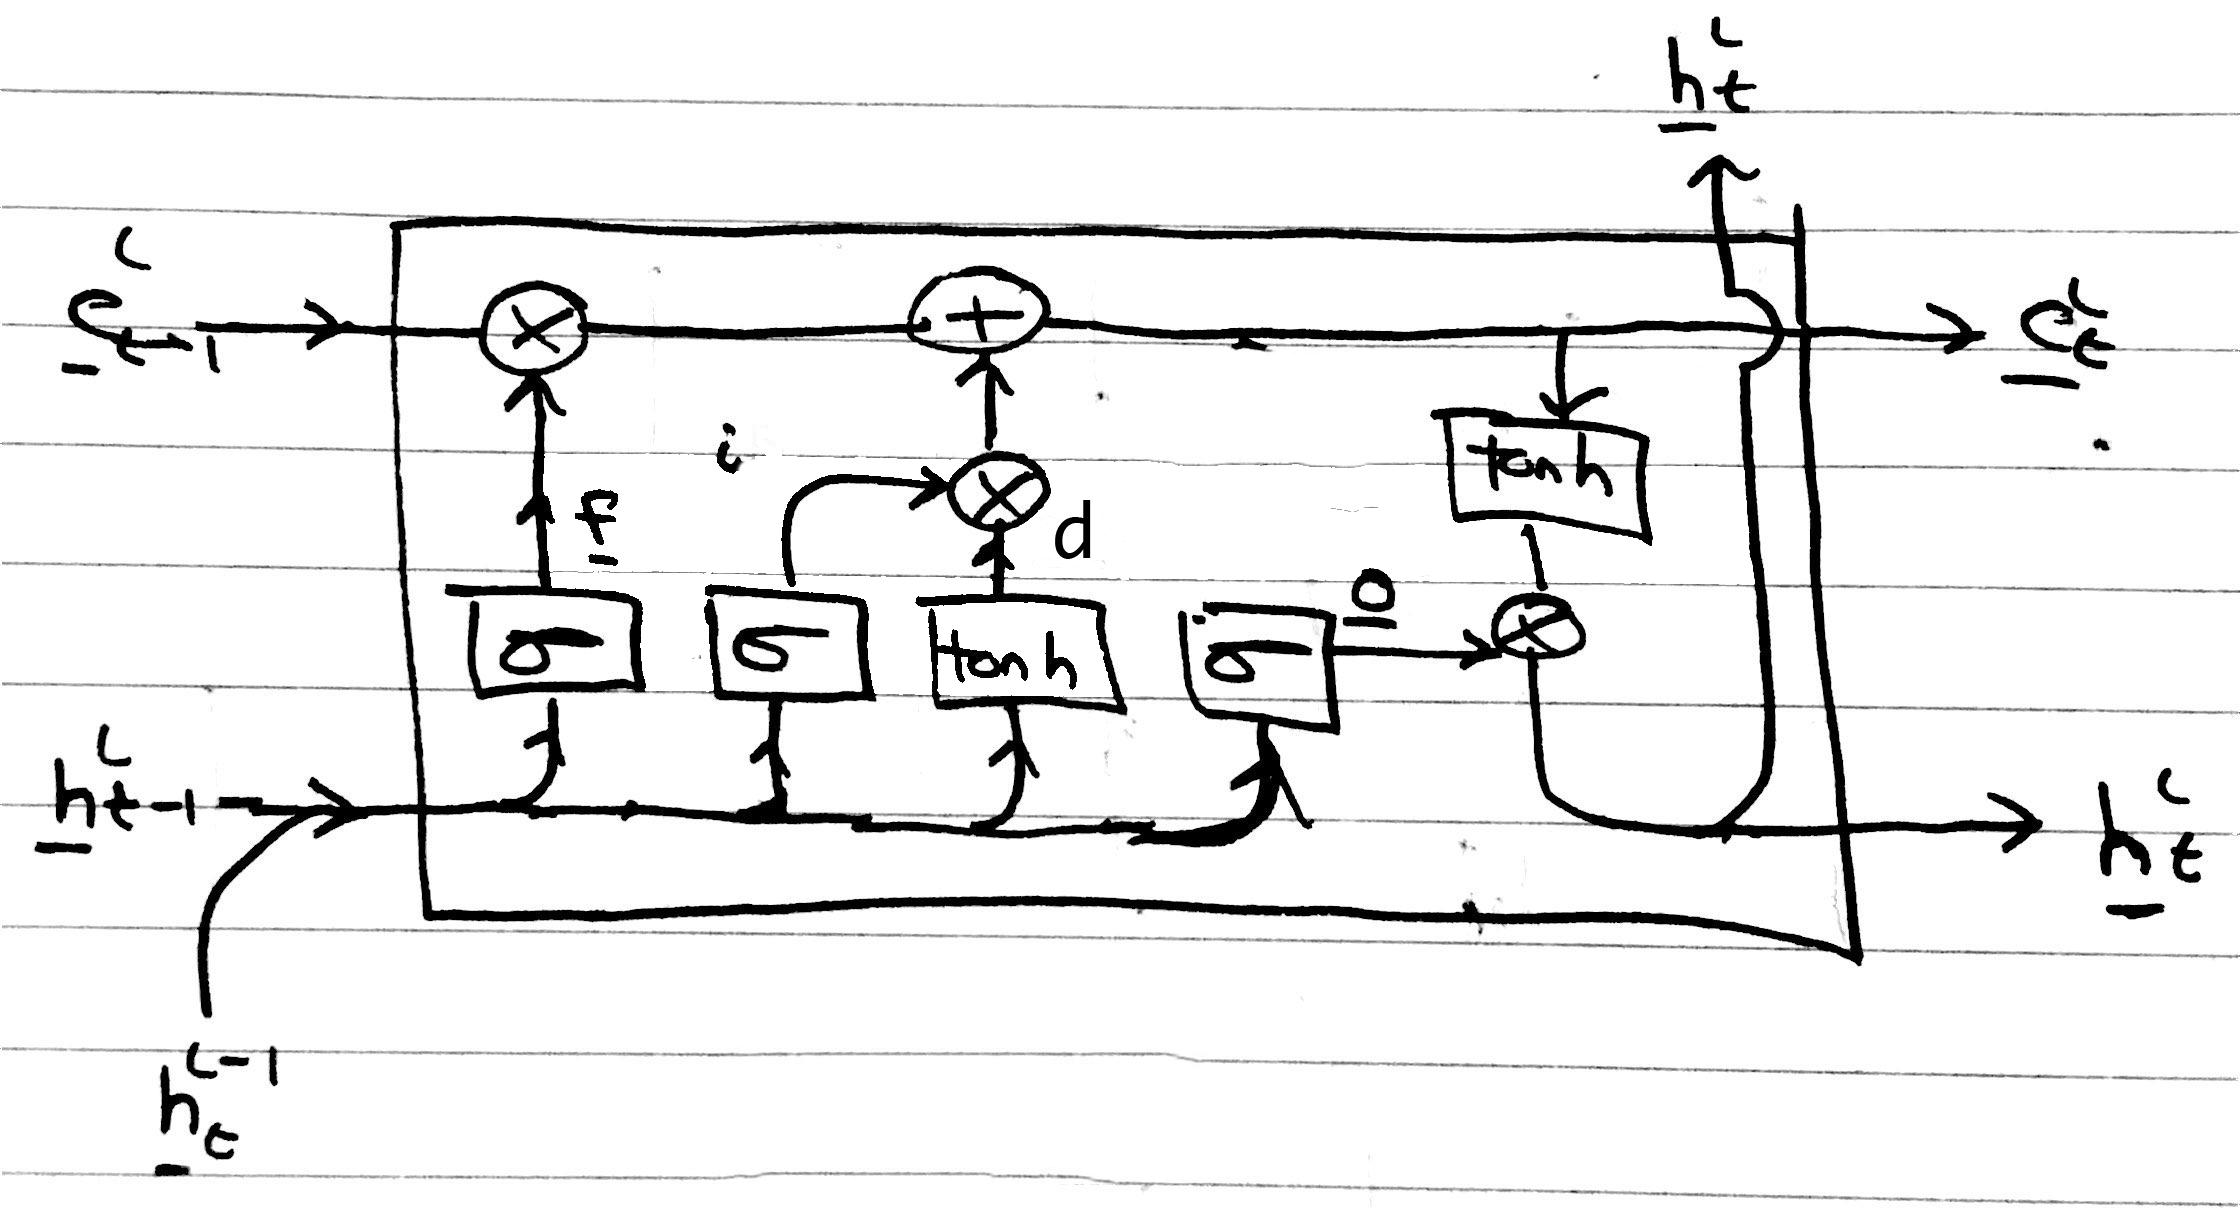
\includegraphics[width=350pt]{figs/lstm_detail_tmp.png}
\caption{LSTM Cell Structure}
\label{fig:lstm-cell}
\end{figure}

\begin{figure}[H]
\centering
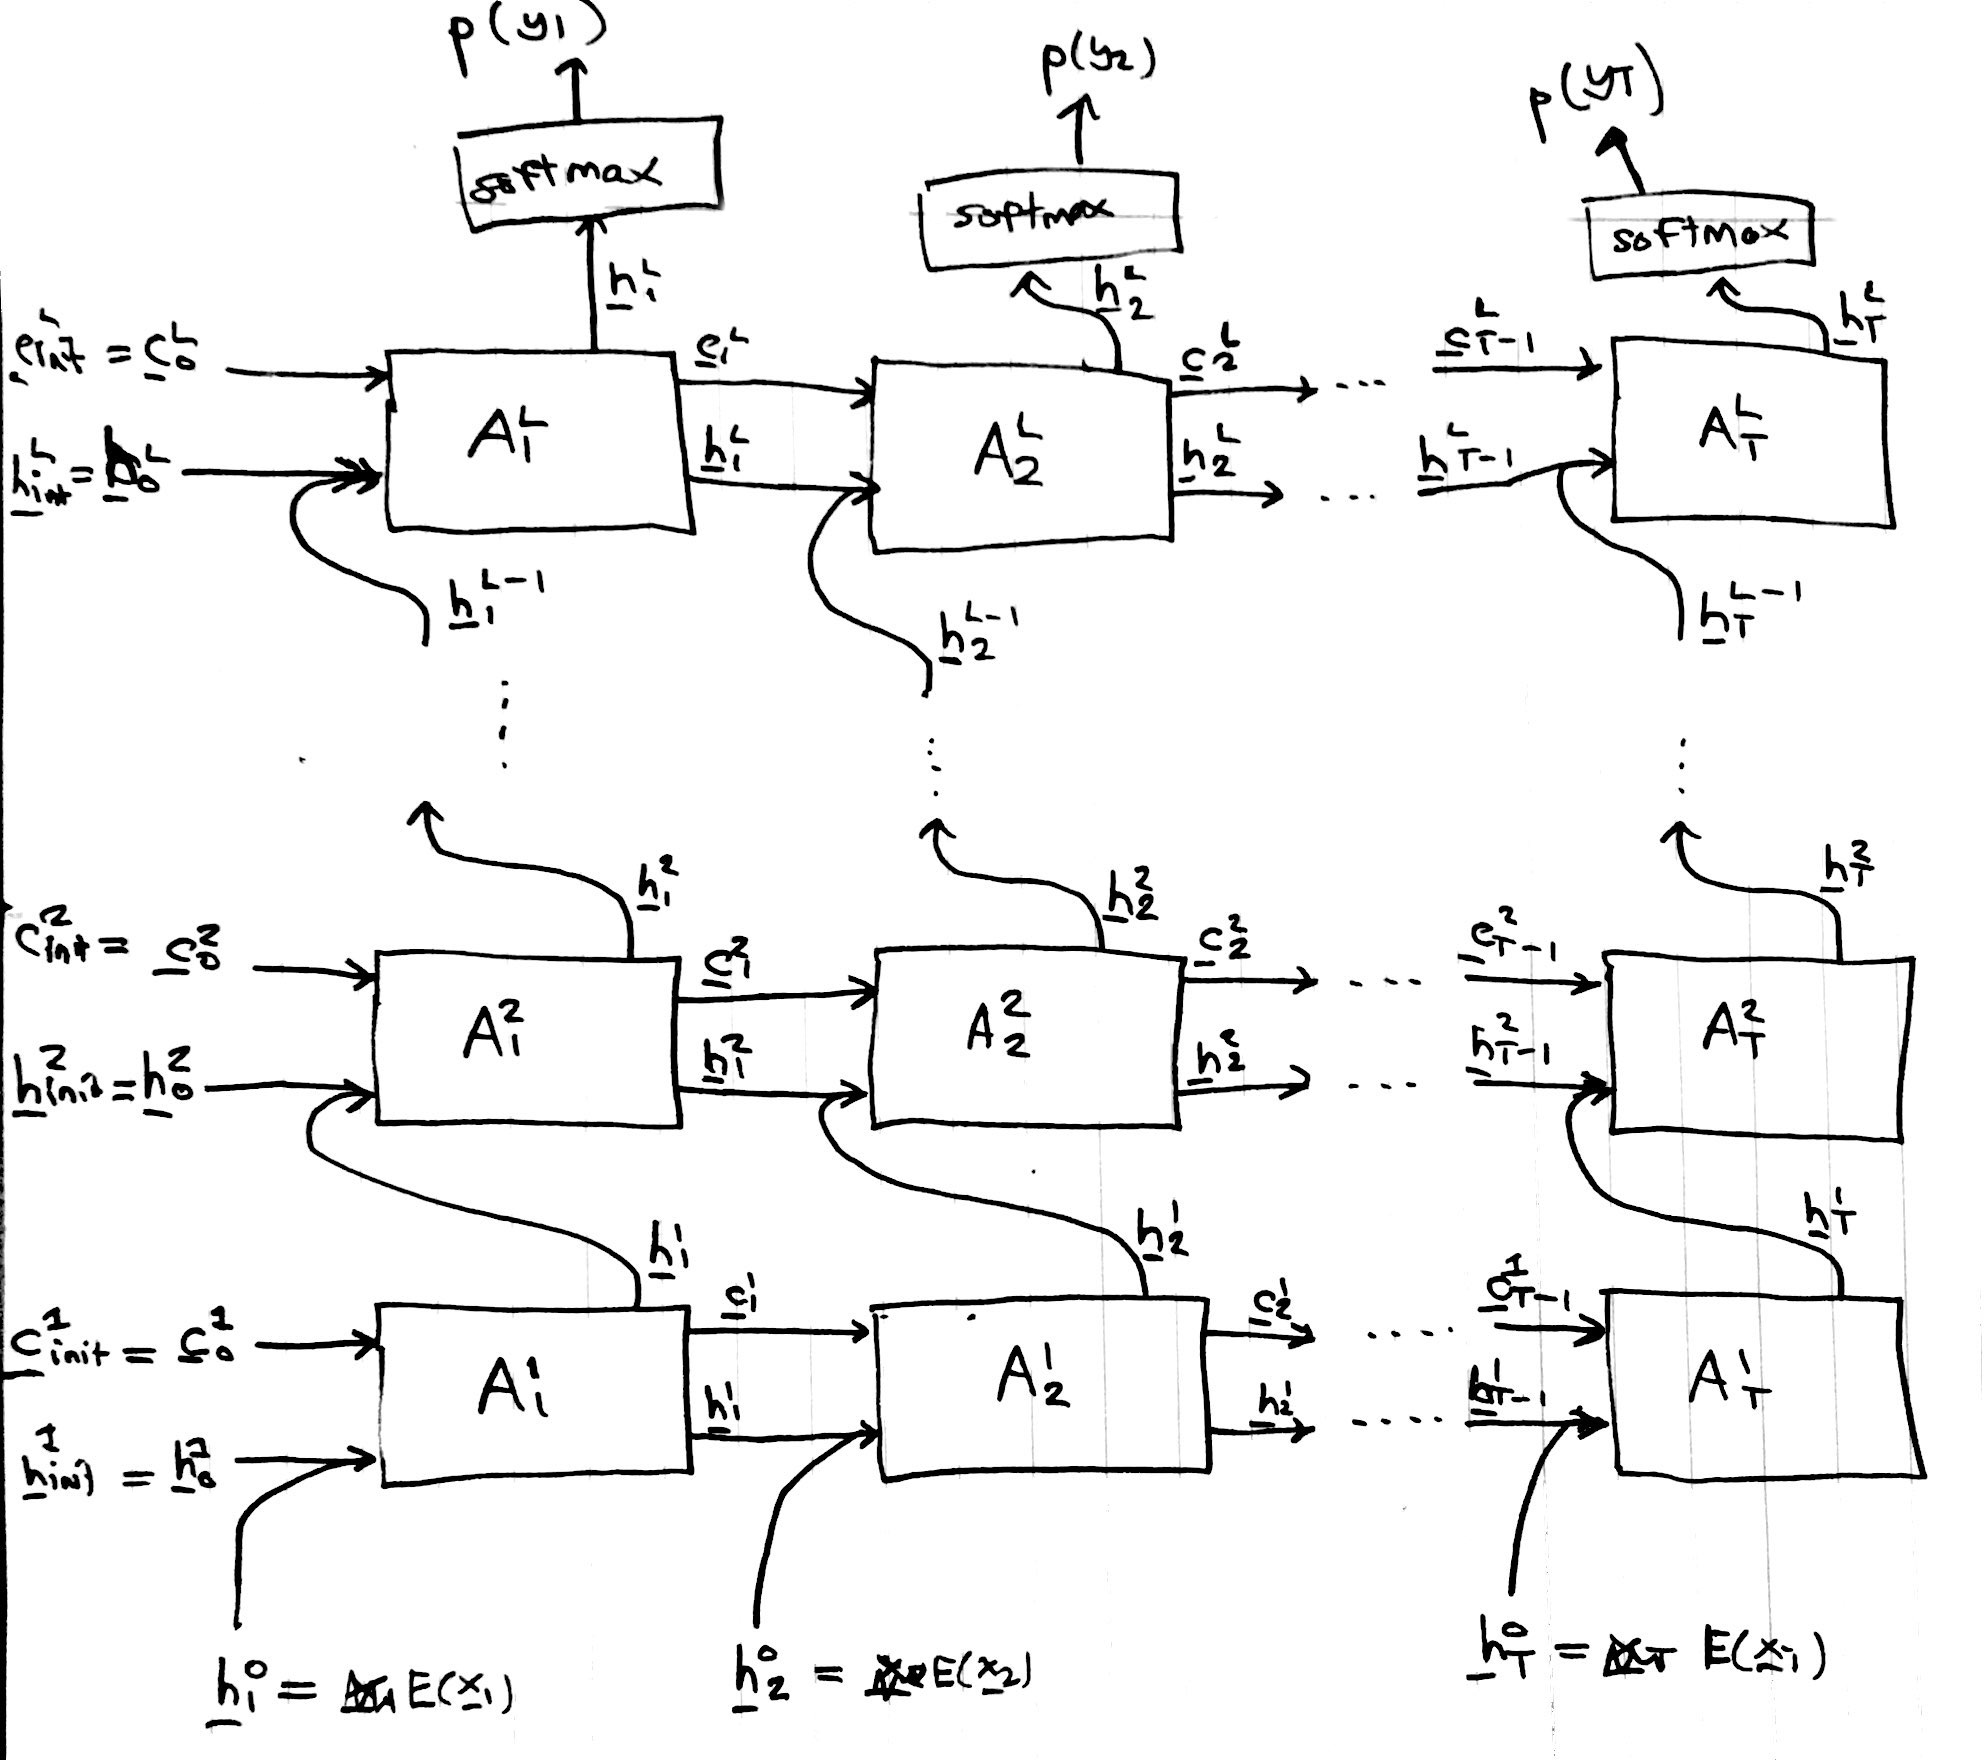
\includegraphics[width=400pt]{figs/lstm_net_tmp.jpg}
\caption{Flow of information in deep LSTM network}
\label{fig:deep-lstm-arch}
\end{figure}

Let $\ast$ denote pointwise vector multiplication. Given input
$\vect{h}_t^{l-1}$, recurrent state $\vect{h}_{t-1}^l$, cell state
$\vect{c}_{t-1}^l$, and writing $\vect{x} = [\vect{h}_{t-1}^l,
\vect{h}_t^{l-1}]$, an LSTM first computes intermediates with equations
(\ref{eq:lstm-f}) through (\ref{eq:lstm-d}).
\begin{align}
  \vect{f} &= \sigma(\vect{W}_f \vect{x} + \vect{b}_f) \label{eq:lstm-f} \\
  \vect{i} &= \sigma(\vect{W}_i \vect{x} + \vect{b}_i) \\
  \vect{o} &= \sigma(\vect{W}_o \vect{x} + \vect{b}_o) \\
  \vect{d} &= \tanh(\vect{W}_d \vect{x} + \vect{b}_d) \label{eq:lstm-d}
\end{align}
The new states $\vect{c}_t^l$ and $\vect{h}_t^l$ are then computed with
equations (\ref{eq:lstm-c}) and (\ref{eq:lstm-h}). 
\begin{align}
  \vect{c}_t^l &= \vect{f} \ast \vect{c}_{t-1}^l + \vect{i} \ast \vect{d}
  \label{eq:lstm-c} \\
  \vect{h}_t^l &= \vect{o} \ast \tanh(\vect{c}_t^l) \label{eq:lstm-h}
\end{align}

As before, parameters are shared across time but not between layers:
superscripts are omitted from the equations for clarity.

The cell state $\vect{c}_t^l$ is intended to act as a memory. The LSTM can be
understood intuitively as using this cell state following three principles of
selectivity:
\begin{enumerate}[label=\arabic*., itemsep=0mm]
  \item \textbf{Write} selectively: only selected information entering the cell
    should be written into the cell state.
  \item \textbf{Read} selectively: only selected information from the cell's
    memory should be included in the output state vector.
  \item \textbf{Forget} selectively: occasionally, previously-useful memories
    will no longer be relevant, and the cell should forget them.
\end{enumerate}

The sigmoidal units $\vect{f}, \vect{i}$, and $\vect{o}$ are known as
\emph{gates}: they scale the activations of other units componentwise and
regulate the flow of information through the cell. The function of each of the
LSTM units can be understood in terms of these principles as follows:

\begin{itemize}
  \item $\vect{f}$ is known as the \emph{forget gate}: it selectively removes
    information from the previous cell state.
  \item The tanh layer $\vect{d}$ is known as the \emph{input feature}. It
    computes data that can be written in the protected cell state.
\item $\vect{i}$ is known as the \emph{input gate}: it controls which data from
  the input feature gets written into the cell state.
\item Finally, $\vect{o}$ is the \emph{output gate}: it regulates which data
  gets output based on the cell state.
\end{itemize}

Note that, since the introduction of LSTM, many other variants have appeared.
For example, an LSTM that also considers the previous cell state
$\vect{c}_{t-1}^l$ when evaluating the gate units (equations (\ref{eq:lstm-f})
through (\ref{eq:lstm-d})) is known as an LSTM with \emph{peephole} connections.
Generally, LSTM variants have only been shown to achieve marginal performance
improvements from the standard LSTM architecture. We shall only consider the
architecture described thus far.

\subsection{Regularisation}

A known problem with neural networks in general is \emph{overfitting}. For deep
feedforward networks, \emph{dropout} \cite{srivastava2014dropout} has seen
significant success in preventing overfitting (regularisation). However, it was
not until the recent work of Zaremba et al.\ \cite{zaremba2014recurrent} that it
was known how to successfully apply dropout to recurrent networks. The authors
determine that applying dropout to only the non-recurrent connections in the
network leads to successful regularisation. 

\section{Choice of Libraries}

To prepare the corpus, I needed a library capable of parsing music notation,
such as MusicXML. The Python package \texttt{music21}, which includes a MusicXML
parser, and is distributed with the chosen corpus in MusicXML form, was
considered ideal for this. 

The other major choice of library was that of a library to assist in the RNN
implementation. I wanted a library where the level of abstraction offers
considerable flexibility, but mundane tasks such as calculating the gradients to
perform the backwards pass through the network during training were handled
automatically. TensorFlow \cite{abadi2016tensorflow}, with its abstraction of
the \emph{computational graph}, was considered the ideal tool for this purpose.

\section{Software Engineering}

An Agile development methodology was adopted to divide the implementation into
orthogonal components which could be completed in two-week sprints and
individually tested. Code reviews were performed with the project supervisor at
the end of each sprint. 

Unit tests were assmebled from hand calculations and data taken from examples in
key papers. Using this method, an error was discovered in the example context
model data from Conklin\ \& Witten's 1995 paper \cite{conklin1995viewpoints}.

\texttt{C++} code was written using modern language features and followed the
\texttt{C++} mantra of \emph{Resource Allocation is Initialisation} (RAII) which
prevented memory leaks in the vast majority of cases. The unique memory leak was
due to a missing virtual destructor in the root of the prediciton stack. This
was debugged using \texttt{valgrind}\footnote{http://valgrind.org/} running
inside a Linux container for reproducibility and due to recent conflicting
changes in macOS, my development platform of choice.

The project and dissertation source code were kept under version control using
Git\footnote{https://git-scm.com/} and pushed to an online
repository\footnote{https://github.com/alexcoplan/p2proj}.

\chapter{Implementation}\label{chap:impl}

\section{Corpus Preparation and Analysis}\label{sec:corpus-prep-analysis}

The high-level description of the chosen representation in
Section~\ref{sec:corp-rep} was made concrete by using a JSON format to encode
the chorales. JSON was chosen due to readily-available library support in both
Python and \texttt{C++}, as well as its human-readable nature, so as to simplify
the debugging process. This JSON format was used for musical I/O of both models.
Figure~\ref{fig:chorale-excerpt} exemplifies this format. 

\vspace{4mm}
\begin{minted}[frame=single, linenos=true, fontsize=\footnotesize]{js}
{
  "title": "Aus meines Herzens Grunde (Excerpt)",
  "bwv": "269",
  "time_sig_amt": 12,
  "key_sig_sharps": 1,
  "notes": [
    [67, 8,  4], [67, 12, 8], [74, 20, 4], [71, 24, 6], 
    [69, 30, 2], [67, 32, 4], [67, 36, 6], [69, 42, 2], 
    [71, 44, 4], [69, 48, 8], [71, 56, 4], [74, 60, 8], 
    [72, 68, 4], [71, 72, 4], [69, 76, 8], [67, 84, 8]
  ]
}
\end{minted}

\begin{figure}[H]
\centering
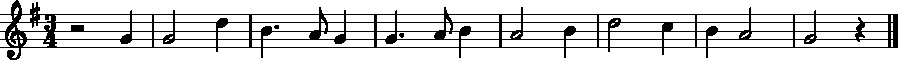
\includegraphics[width=450pt]{figs/aus_meines_excerpt.pdf}
\caption{JSON Chorale excerpt with corresponding score}
\label{fig:chorale-excerpt}
\end{figure}

Analysis was performed on the corpus in order to better understand its musical
characteristics. This informed the construction of \texttt{C++} classes to
represent musical types, as well as corpus preprocessing techniques utilisted in
the RNN implementation. Figures~\ref{fig:key-dist} and \ref{fig:range-dist}
demonstrate this analysis.

Tonality metadata was extracted in the form of key signatures represented as
integers in $[-7,7]$, where a positive number indicates the sharps, and a
negative number flats. Time signatures are represented as the number of
semiquavers in a bar, which suffices to distinguish \lilyTimeSignature{3}{4} and
\lilyTimeSignature{4}{4}, the two time signatures used in the chorales.

\begin{figure}[H]
\centering
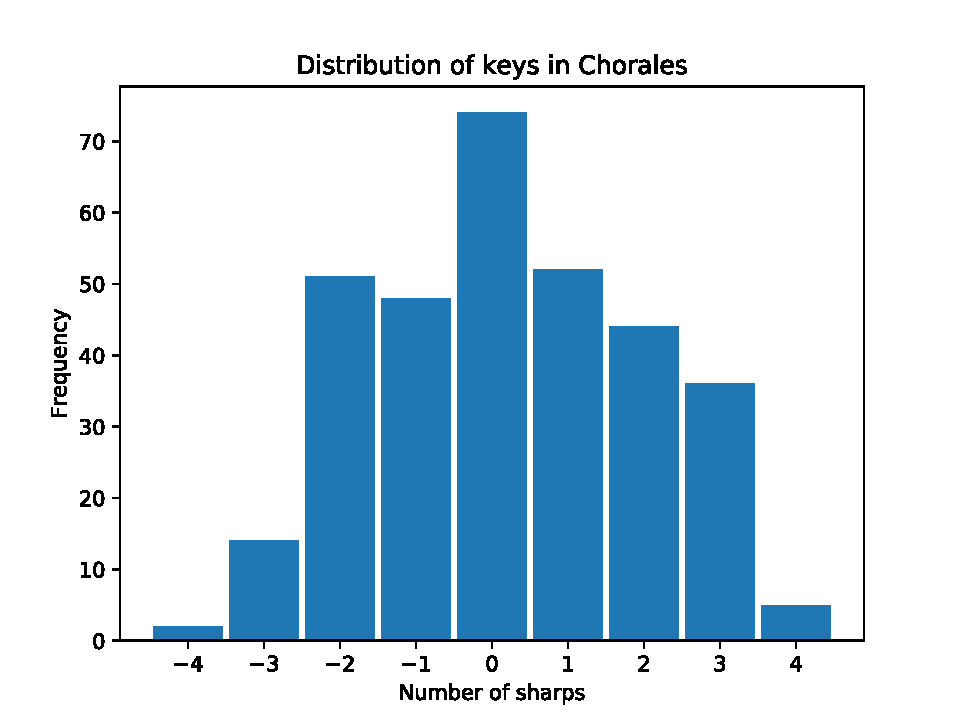
\includegraphics[width=300pt]{figs/key_dist.pdf}
\caption{Histogram showing distribution of key signatures in corpus}
\label{fig:key-dist}
\end{figure}

\begin{figure}[H]
\centering
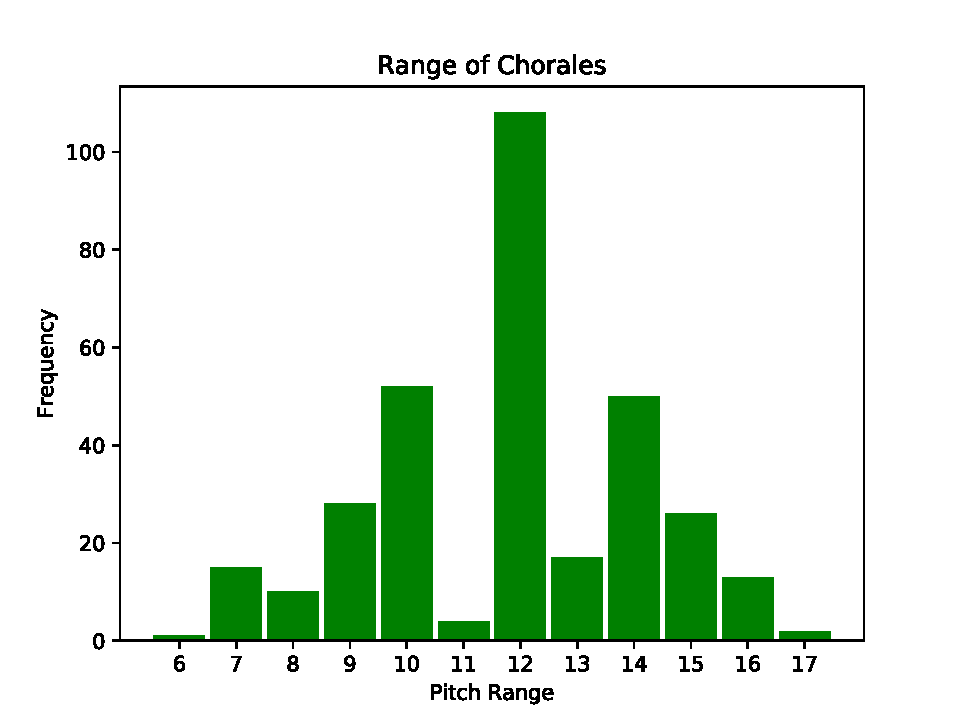
\includegraphics[width=300pt]{figs/range_dist.pdf}
\caption{Histogram showing distribution of pitch range in chorales}
\label{fig:range-dist}
\end{figure}

\section{Multiple Viewpoint System}

\subsection{Overview}

\begin{figure}[H]
\centering
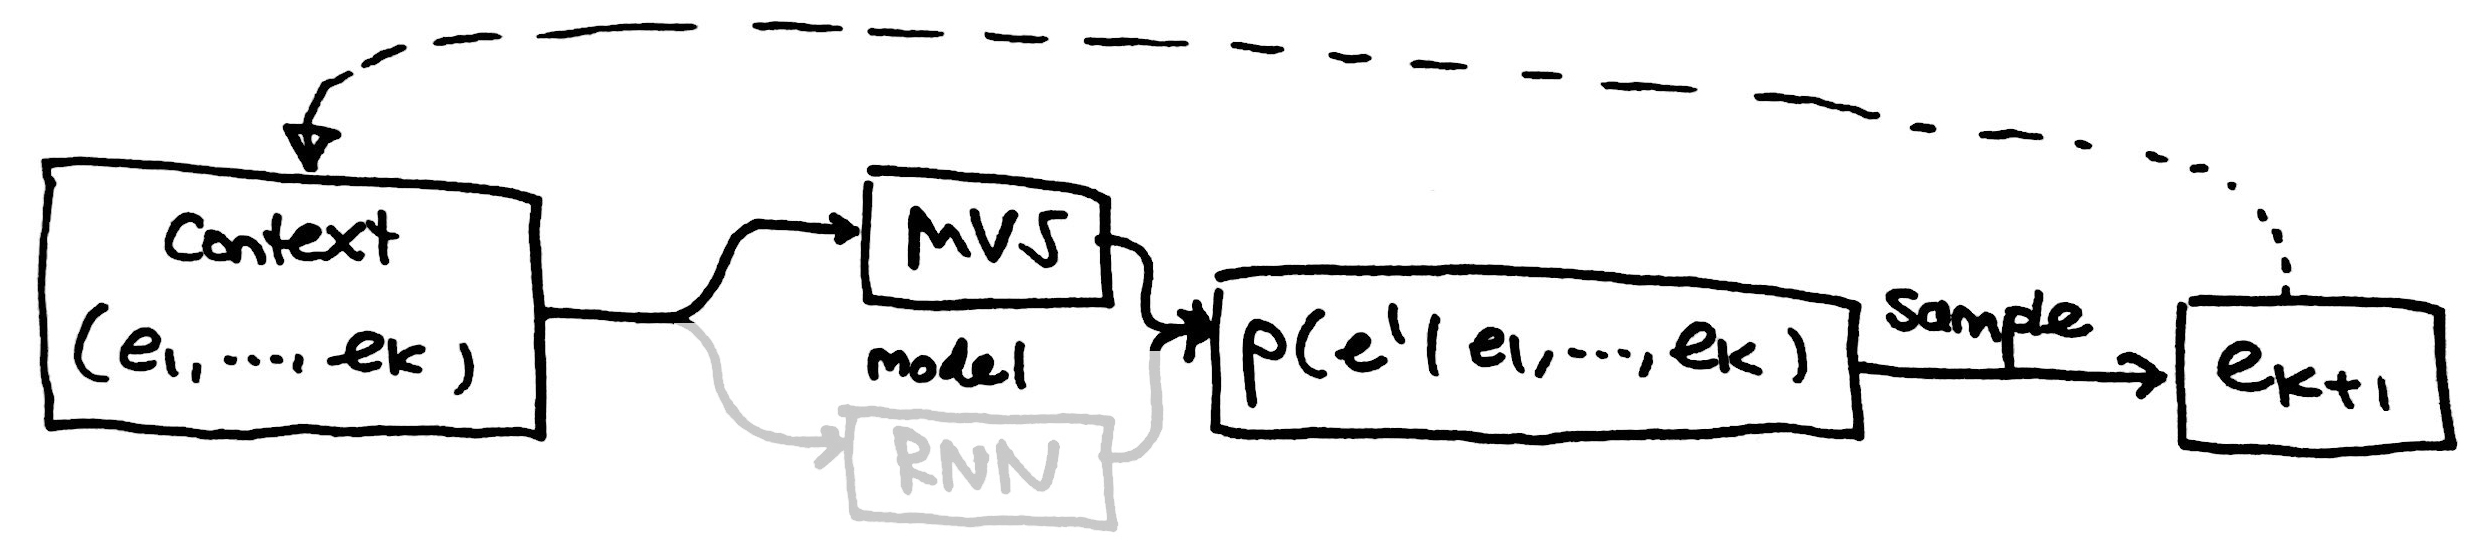
\includegraphics[width=400pt]{figs/high_level_mvs_tmp.jpg}
\caption{Overview of music generation using MVS}
\label{fig:mvs-gen-overview}
\end{figure}

A complete framework for implementing Multiple Viewpoint Systems in \verb!C++!
has been implemented and released as an open source project for others to use.
Since no existing framework was available, this had to be implemented from
scratch. The framework implements the formalism detailed in
Section~\ref{sec:mvs-formalism} in full. I chose to make the implementation as
general as possible so that it may be of use in other contexts in the future. 

This general framework was then specialised to model the chorales. At the core
of the framework, the \emph{prediction by partial match} (PPM) algorithm was
implemented for smoothing variable-order context models. The distributions
predicted by these context models are combined using the entropy-weighted
schemes described in Section~\ref{sec:vp-comb}.

Abstractions were made such that, using these primitives, \emph{basic},
\emph{derived}, \emph{linked}, and \emph{triply-linked} viewpoints can be
instantiated over arbitrary combinations of types. Both a \emph{long-term} model
and \emph{short-term} were implemented.  Sampling by iterative random walk was
implemented for melody generation. Finally, an automatic viewpoint selection
algorithm in the form of \emph{forward step-wise selection}
\cite{pearce2005construction} was implemented.

The principal design strategy of the implementation was to achieve a tight
correspondence between the \texttt{C++} type system and the formalism of
multiple viewpoints detailed in Section~\ref{sec:mvs-formalism}. This was
considered desirable for two main reasons:
\begin{itemize}
  \item A correspondence between the \texttt{C++} type system and MVS formalism
    provides the basis for an API that should be intelligible by both
    \texttt{C++} programmers and those familiar with the formalism.
  \item Making full use of the type system in a statically-typed language 
    enables many more potential programmer errors to be caught at compile time.
\end{itemize}

\texttt{C++} templates were considered the ideal tool to achieve this. Templates
are \emph{flexible}, allow for considerable \emph{generality}, and are evaluated
at compile time, thereby achieving better safety guarantees.

\begin{figure}[H]
\centering
  \trimbox{0cm 2.5cm 0cm 0cm}{ 
  \begin{tikzpicture}
  \umlclass[type=interface, template={$\zeta$,
    $T_{\text{predict}}$}]{Predictor}{}{
    +predict(context : $\zeta^*$) : dist$\langle T_{\text{predict}}
    \rangle$  \\
    +learn(sequence : $\zeta^*$)
  }
  \umlsimpleclass[y=-4, template={$\zeta$, $T_{\text{viewpoint}}$}]{GeneralViewpoint}
  \umlsimpleclass[x=9, template={$\zeta$, $T_l$, $T_r$}]{GeneralLinkedVP}

  \umlsimpleclass[x=9,y=-4, alias=seqspeclink]{SequenceModel}
  \umlsimpleclass[y=-7, alias=seqspec]{SequenceModel}
  \umlsimpleclass[y=-7,x=9, template={$T$}, alias=seqgen]{SequenceModel}
  \umlsimpleclass[y=-10,x=9, alias=ctxspec]{ContextModel}
  \umlsimpleclass[y=-10, alias=ctxgen, template={$b$}]{ContextModel}
  \umlsimpleclass[y=-13]{TrieNode}
  
  \umlimpl{GeneralViewpoint}{Predictor}
  \umlimpl{GeneralLinkedVP}{Predictor}

  \umlunicompo[arg=model, mult=1]{GeneralViewpoint}{seqspec}
  \umlunicompo[arg=model, mult=1]{GeneralLinkedVP}{seqspeclink}
  \umlreal[stereo={$T \rightarrow T_{\text{viewpoint}}$}]{seqspec}{seqgen}
  \umlreal[stereo={$T \rightarrow \text{Pair}\langle T_l, T_r
  \rangle$}]{seqspeclink}{seqgen}
  
  \umlunicompo[arg=model, mult=1]{seqgen}{ctxspec}
  \umlreal[stereo={$b \rightarrow T::\text{cardinality}$}]{ctxspec}{ctxgen}

  \umlunicompo[arg=trie root, mult=1]{ctxgen}{TrieNode}
  \umlunicompo[arg=children, mult=0..b, recursive=-90|2|3cm]{TrieNode}{TrieNode}
\end{tikzpicture}
}
\hspace{-10mm}
\caption{UML Class Diagram of Prediction Stack}
\label{fig:uml-prediction}
\end{figure}

Despite templates being the primary means of achieving polymorphism, inheritance
polymorphism is used to implement an abstract base class for viewpoints
(Figure~\ref{fig:uml-prediction}). This was done in order to unify the
otherwise-heterogeneous viewpoint types predicting each basic type. For example,
viewpoints $\emph{duration} \otimes \emph{pitch}$, \emph{seqint}, and
\emph{pitch} have different types, but are all predictors of pitch: we want to
refer to them polymorphically as such.

\begin{figure}[H]
\centering
  \trimbox{0cm 0.0cm 0cm 0cm}{ 
  \begin{tikzpicture}
  
  \umlclass{ChoraleMVS}{
    - short\_term\_layer : ChoraleVPLayer \\
    - long\_term\_layer : ChoraleVPLayer
  }{
    + add\_viewpoint$\langle T \rangle$(vp : ChoralePredictor$\langle T\rangle$ *) \\
    + predict$\langle T\rangle$(context : vec$\langle$ChoraleEvent$\rangle$) :
    dist$\langle T \rangle$ \\
    + cross\_entropy(seq : vec$\langle$ChoraleEvent$\rangle$) : double \\
    + generate(length : int, ts : TimeSig) : vec$\langle$ChoraleEvent$\rangle$
    \\
    + learn(example : vec$\langle$ChoraleEvent$\rangle$)
  }
  \umlsimpleclass[y=-5]{ChoraleVPLayer}
  \umlsimpleclass[x=-5, y = -9, alias=pitchpred]{Predictor}
  \umlsimpleclass[x=0, y = -9, alias=durpred]{Predictor}
  \umlsimpleclass[x=5, y = -9, alias=restpred]{Predictor}
  \umlsimpleclass[y = -13, type=interface, template={$T$}, alias=cpred]{Predictor}
  \umlsimpleclass[y = -17, type=interface, template={$\zeta$, $T$},
alias=predbase]{Predictor}
  
  \umlunicompo[arg=short-term, mult=1, anchors=-115 and 160]{ChoraleMVS}{ChoraleVPLayer} 
  \umlunicompo[arg=long-term, mult=1, anchors=-65 and 20]{ChoraleMVS}{ChoraleVPLayer}
  \umluniaggreg[arg=pitch\_vps, mult=1..*]{ChoraleVPLayer}{pitchpred}
  \umluniaggreg[arg=duration\_vps, mult=1..*]{ChoraleVPLayer}{durpred}
  \umluniaggreg[arg=rest\_vps, mult=1..*]{ChoraleVPLayer}{restpred}
  \umlreal[stereo={$T \rightarrow$ ChoralePitch}, pos stereo=0.3]{pitchpred}{cpred}
  \umlreal[stereo={$T \rightarrow$ ChoraleDuration}, pos stereo=0.55]{durpred}{cpred}
  \umlreal[stereo={$T \rightarrow$ ChoraleRest}, pos stereo=0.3]{restpred}{cpred}
  \umlreal[stereo={$\zeta \rightarrow$ ChoraleEvent}]{cpred}{predbase}
\end{tikzpicture}
}
\hspace{-10mm}
\caption{UML Class Diagram relating viewpoint framework with Chorale
hierarchy}
\label{fig:chorale-uml}
\end{figure}

We now give a brief overview of the main components to gain an appreciation of
the intent behind each component before taking a closer look at various parts of
the implementation.

\begin{itemize}
  \item \texttt{TrieNode<b>} implements a trie with branching factor \texttt{b}.
  \item Using this data structure, \texttt{ContextModel<b>} implements a context
    model over an alphabet of size \texttt{b}, as per
    Section~\ref{sec:ctx-model-prep}.   
  \item A unified representation for domain-specific types is used throughout.
    Examples include basic types such as \texttt{ChoralePitch} and
    \texttt{ChoraleDuration}, derived types such as \texttt{ChoraleInterval} and
    meta-types such as \texttt{EventPair<T1,T2>}.
  \item \texttt{SequenceModel<T>} further abstracts \texttt{ContextModel} by
    implementing a higher-level interface to context models in terms of these
    domain-specific types.
  \item \texttt{EventDistribution<T>} represents a probability distribution over
    a type \texttt{T}. It supports random sampling as well as multiple
    distribution combination schemes as per Section~\ref{sec:vp-comb}. Objects
    of this type are returned by \texttt{SequenceModel} objects when predicting
    the next event in a sequence.
  \item All viewpoints implement the \texttt{Predictor<EventSpace,T>} template
    interface. These are outlined in Figure~\ref{fig:uml-prediction}. Such
    objects contain an underlying \texttt{SequenceModel} object and support the
    operations of \emph{lifting} and \emph{reification} as per
    Section~\ref{sec:mvs-formalism}.
  \item \texttt{ChoraleVPLayer} is a container for sets of viewpoints over the
    chorale-specific types, used to implement both the \emph{long-term} and
    \emph{short-term} model.
  \item Finally, \texttt{ChoraleMVS} is a high-level class which manages all the
    components of a MVS over chorales and provides a unified interface for tasks
    such as \emph{prediction} and \emph{generation}.
    Figure~\ref{fig:chorale-uml} illustrates how these components relate to each
    other.
\end{itemize}

\subsection{Context Models}

Recall from Section~\ref{sec:ctx-model-prep} that a context model populates a
database of examples during training and subsequently uses an inference
procedure to perform prediction by matching contexts against the database. We
first tackle the construction of the underlying data structure, and then turn to
inference.

The procedure for extracting $h$-grams from an example sequence $e_1^k$is
detailed in Algorithm~\ref{alg:sliding-window}.

\begin{algorithm}[H]
  \caption{Sliding window algorithm for $h$-gram extraction}
  \label{alg:sliding-window}
  \begin{algorithmic}[1]
    \Function{learn-sequence}{$e_1^k \in [\tau]^*$}
      \For{$j : 1 \rightarrow k$}
      \Comment $j$: window end position
        \State \Call{add-or-increment}{()}
        \For{$i : \min(1,j - \hbar + 1) \rightarrow j$} 
        \Comment $i$: window start position
          \State \Call{add-or-increment}{$e_i^j$}
        \EndFor
      \EndFor
    \EndFunction
  \end{algorithmic}
\end{algorithm}

The function \Call{add-or-increment}{$e_i^j$} looks up $e_i^j$ in the trie. If
found, its count is incremented. Otherwise, $e_i^j$ is inserted into the trie,
the resulting node initialised with a count of unity. Note that $()$, the empty
sequence, corresponds to the root node in the trie. 

While this algorithm can be used to train a long-term model, a short-term model
requires a context model that can be updated online during sequence prediction.
Therefore, context models also implement a method which extracts just those
$h$-grams at the tail of the sequence (with the window at the far right).

\subsubsection{Implementing PPM}\label{subsec:ppm-imp}

Recall from the discussion in Section~\ref{sec:ctx-model-prep} that care must be
taken to ensure the normalisation of distributions predicted by PPM.
Algorithm~\ref{alg:ppm-a} details pseudocode for PPM A with exclusion which I
derived from high-level descriptions in the literature. 

The key to exclusion in this algorithm is the \textit{Dead} set that is
maintained throughout the recursion. This set is initialised to $\varnothing$
and later populated with those events that we \emph{could} have matched at a
higher-order model and therefore no longer need to consider at lower-order
models. To compute $\mathbb{P}(e' | e_1^k)$ we call \Call{ppm-a}{$e_1^k$, $e'$,
$1$, $\varnothing$}.

\begin{algorithm}[H]
  \caption{PPM A with exclusion}
  \label{alg:ppm-a}
  \begin{algorithmic}[1]
    \Function{ppm-a}{$e_1^k \in [\tau]^*$, $e' \in [\tau]$, $i_{\mathrm{begin}}$, 
    $\textit{Dead} \subseteq [\tau]$}
      \State $\textit{Alive} \gets [\tau] \setminus \textit{Dead}$
      \If{$i_{\mathrm{begin}} > k$}
      \State \Return $1 / |\textit{Alive}|$ \Comment{Base case: uniform
      distribution}
      \EndIf
      \State $i \gets i_{\mathrm{begin}}$
      \For{$i : i_{\mathrm{begin}} \rightarrow k$}
      \If{$C(e_i^k) > 0$} \textbf{break}
      \Comment{Find longest context match}
        \EndIf       
      \EndFor 
      \State $\textit{Known} \gets \set{ e'' \in [\tau]\ |\ C(e_i^k :: e'') > 0 }$
      \State $\textit{Novel} \gets Alive \setminus Known$ \Comment{All
      events we could escape for}
      \State $s \gets \sum_{e'' \in \textit{Alive}} C(e_i^k :: e'')$ 
      \If{$\textit{Novel} = \varnothing$}
        \State \Return $C(e_i^k :: e') / s$ \Comment{No possible need for escape}
      \EndIf
      \If{$e' \in \textit{Known}$}
      \State \Return $C(e_i^k::e') / (1 + s)$ \Comment{Matched $e_i^k::e'$}
      \EndIf
      \State \Return \Call{ppm-a}{$e_1^k$, $e'$, $i+1$, $Dead \cup Known$}$ / (1
      + s)$ \Comment{Escape recursively}
    \EndFunction
  \end{algorithmic}
\end{algorithm}

To realise this pseudocode in \texttt{C++}, the PPM implementation in a
\texttt{ContextModel<b>} instance utilises bitvectors implemented using
\texttt{std::bitset<b>} to efficiently represent sets of nodes. This improves on
alternatives such as \texttt{std::array<b, bool>} in both space and time:
typical implementations pack bits into machine words and implement the bitwise
operations directly.

Figure~\ref{fig:ppm-stepwise} shows the step-by-step execution of this algorithm
computing $\mathbb{P}(\beta|\alpha\gamma)$ on a context model over the alphabet
$\Sigma = \set{\alpha,\beta,\gamma,\delta}$ having seen the training sequence
$(\alpha,\beta,\gamma,\delta,\alpha,\gamma,\alpha,\delta)$.

\begin{figure}[H]
\centering
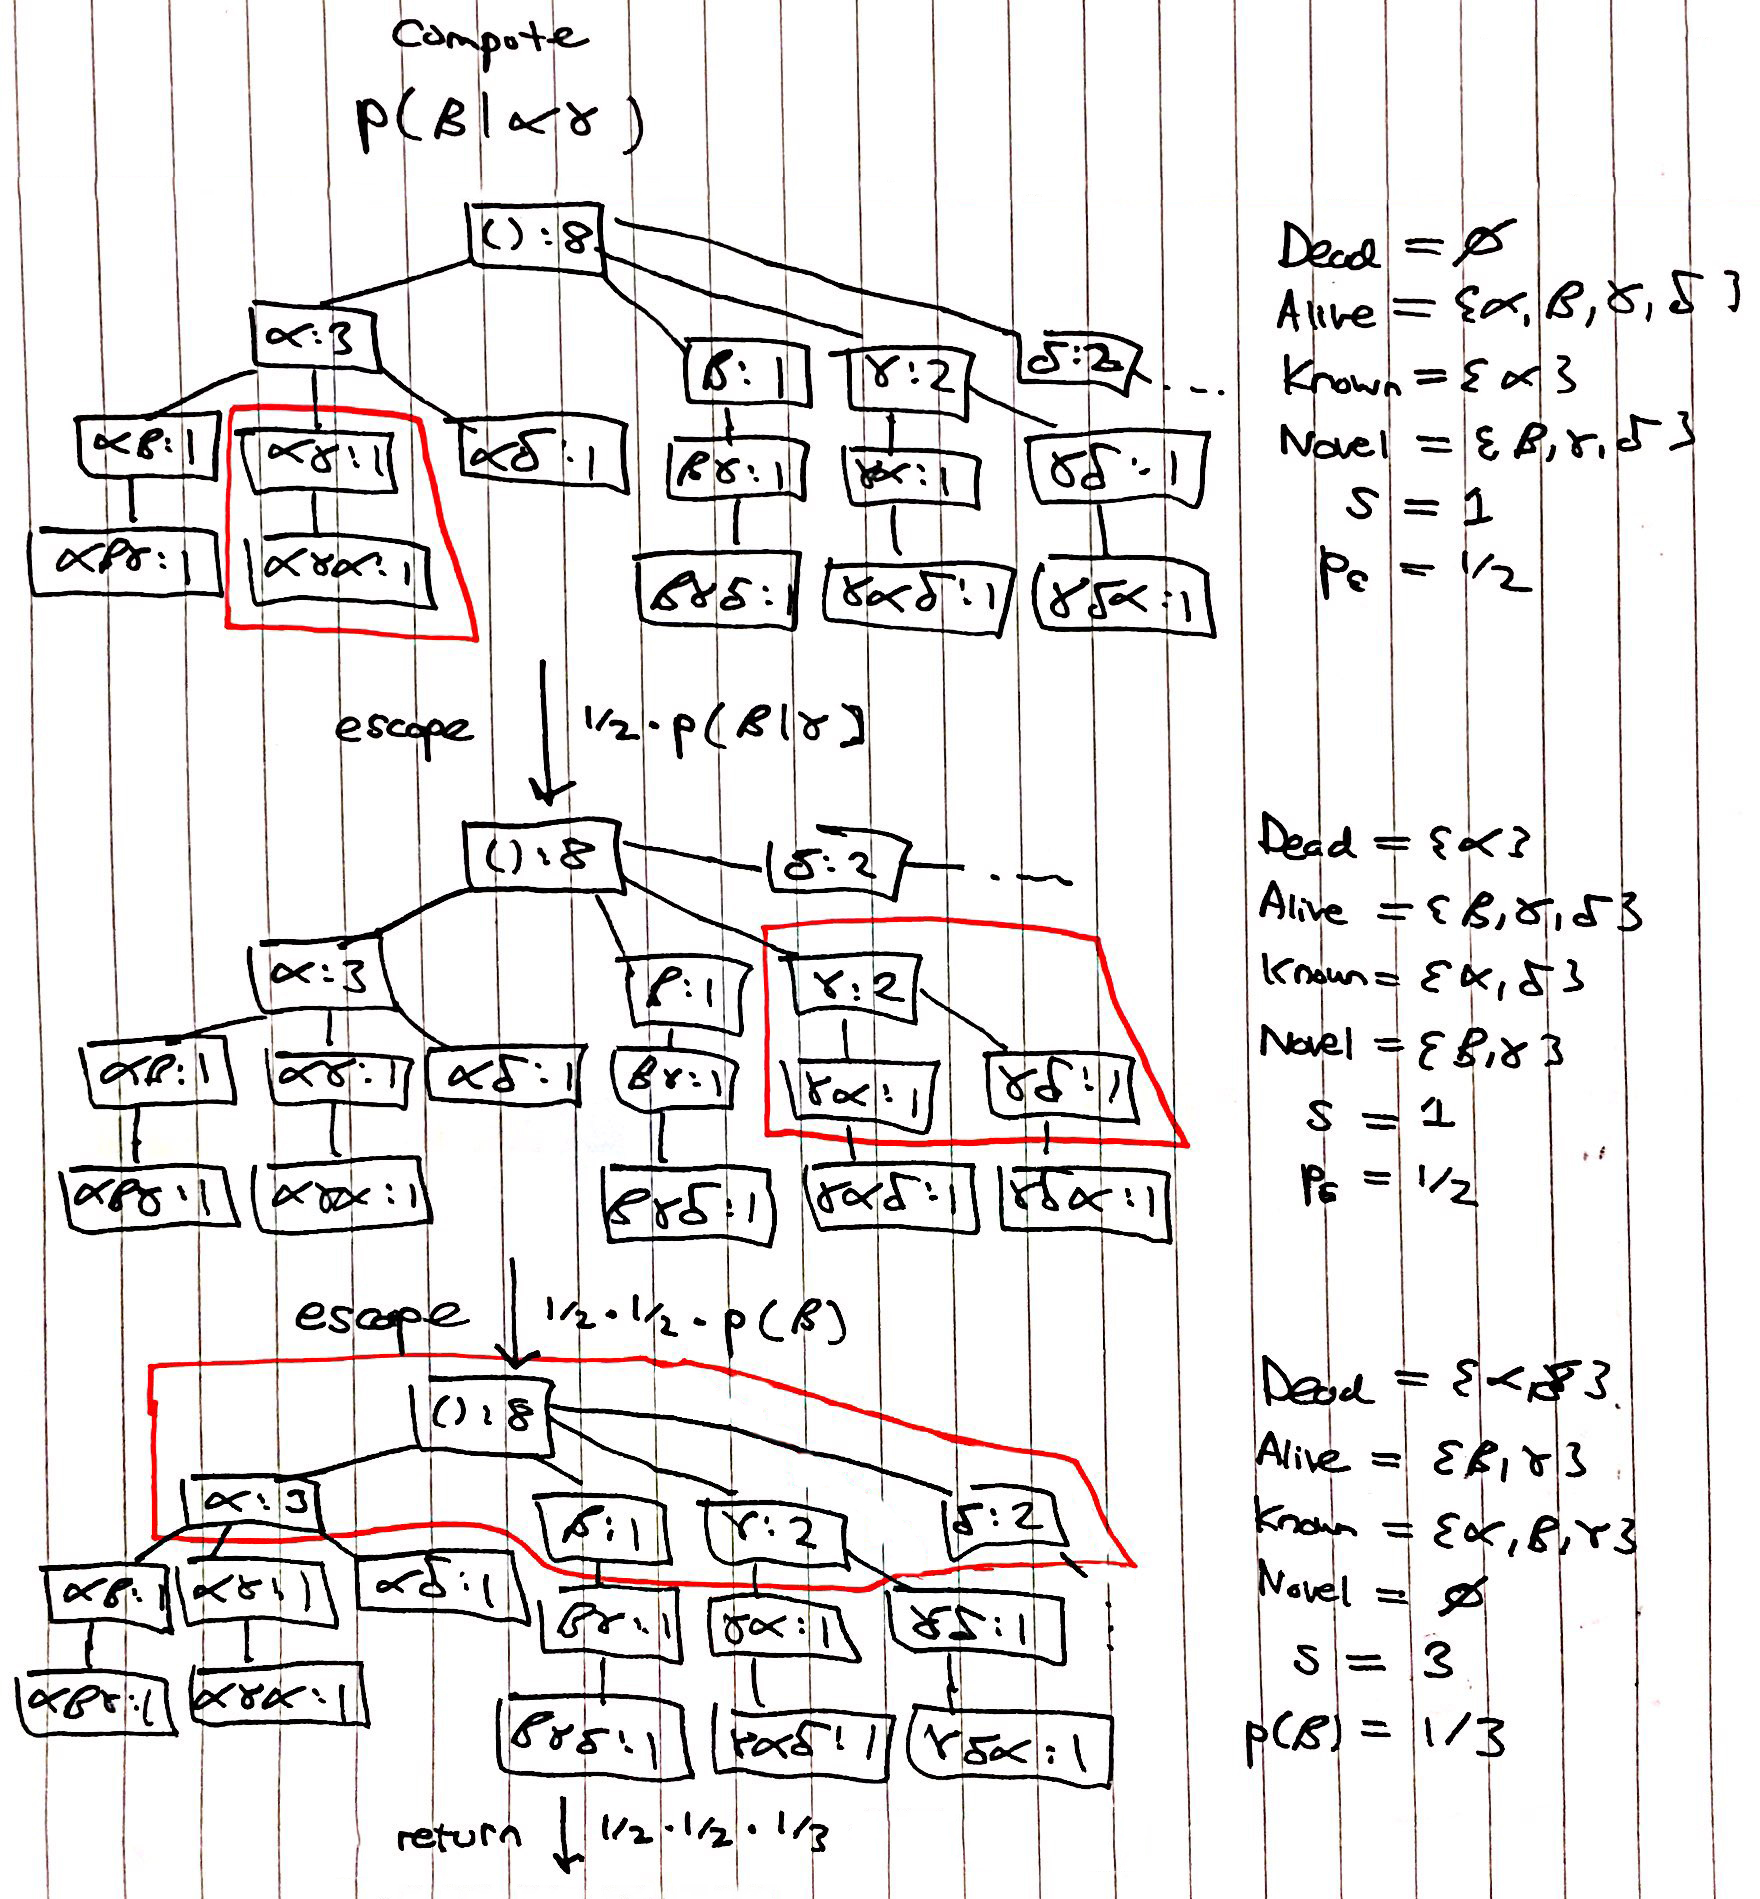
\includegraphics[width=400pt]{figs/ppm_stepwise_tmp.jpg}
\caption{Step-by-step execution of PPM with $\hbar = 3$}
\label{fig:ppm-stepwise}
\end{figure}

Observe that Algorithm~\ref{alg:ppm-a} has time complexity $O(\hbar|[\tau]|)$.
To form a full distribution over $\tau$ requires $|[\tau]|$ iterations of this
algorithm giving a quadratic complexity of $O(\hbar|[\tau]|^2)$. After
completing and profiling the implementation, I realised that PPM can in fact
generate this distribution in linear time by constructing the entire
distribution simultaneously.

\subsection{Event Representation}\label{sec:cpp-event-rep}

In order to abstract the low-level \texttt{ContextModel} implementation and to
represent viewpoint types as first-class citizens in \texttt{C++}, a simple
scheme was devised to represent viewpoint types as classes.

\begin{listing}[H]
  \begin{minted}[frame=single, linenos=true, fontsize=\footnotesize, mathescape]{cpp}
class T {
  const static cardinality; // set to $|[\tau]|$
  unsigned int encode();    // specifies the enumeration

  T(unsigned int c);        // construct using code $0 \leq c < |[\tau]|$
  T(const Other &o);        // construct using data 
};
  \end{minted}
  \caption{Prototypical viewpoint type representation}
  \label{lst:event-rep}
\end{listing}

To interface with the context model implementation, it suffices for each
viewpoint type $\tau$ to specify a well-known enumeration of $[\tau]$. The class
outlined in Listing~\ref{lst:event-rep} is a minimal example of how a class can
conform to this type representation convention.

Many templates in the implementation accept viewpoint types represented in this
way. I also chose to implement an iterator \texttt{EventEnumerator<T>} to
conveniently iterate over the members of a type in the style of the iterators in
the \texttt{C++11} standard template library, enabling clean loops such as~
\cppi{for (auto event : EventEnumerator<T>())}.

\subsection{Abstracting Context Models}

Now that we have established a scheme for representing viewpoint types, we can
abstract context models by providing an interface in terms of viewpoint types.
This is the job of a class which we call \texttt{SequenceModel}.  Specifically,
\texttt{SequenceModel<T>} is a wrapper around an instance of
\texttt{ContextModel<T::cardinality>} for \texttt{T} a viewpoint type
represented as per Section~\ref{sec:cpp-event-rep}. 

Additionally, given some context, \texttt{SequenceModel<T>} objects generate
probability distributions over subsequent events by iterating the PPM
implementation of the underlying context model for each member of \texttt{T}.
The object returned from this operation is an instance of
\texttt{EventDistribution<T>}, the functionality of which is discussed in the
following two sections.

It is desirable to provide an interface to context models in terms of viewpoint
types, since all other high-level classes in the implementation are
parameterised on types. Any viewpoint class modelling an underlying type
\texttt{T} can therefore simply instantiate a \texttt{SequenceModel<T>} object.

\subsection{Distribution Combination}

There are various techniques for combining probability distributions in a MVS.
In line with the Agile development methodology, I initially implemented an
entropy-weighted arithmetic combination scheme in order to get a working result
at an early stage. Later, on the basis of its superior performance
(Section~\ref{sec:vp-comb}), I decided to implement a geometric scheme for
viewpoint combination.  

In order to cleanly express distribution combination with a standard interface,
yet allow the choice of a different underlying implementation, I utilised the
\emph{Strategy} pattern of object-oriented design
(Figure~\ref{fig:dist-strategy-uml}).

\begin{figure}[H]
\centering
  \trimbox{0cm 0.0cm 0cm 0cm}{ 
  \begin{tikzpicture}
  
  \umlclass[type=interface, template={$T$}, alias=strat]{DistCombStrategy}{}{
  + combine(list$\langle$EventDistribution$\langle T \rangle\rangle$) :
  EventDistribution$\langle T \rangle$
  }
  \umlsimpleclass[y = -4, x=-5, template={$T$}, alias=arith]{ArithmeticComb}
  \umlsimpleclass[y = -4, x=0, template={$T$}, alias=geo]{GeometricComb}
  \umlsimpleclass[y = -4, x=5, template={$T$}, alias=loggeo]{LogGeoComb}
  
  \umlimpl{arith}{strat}
  \umlimpl{geo}{strat}
  \umlimpl{loggeo}{strat}
\end{tikzpicture}
}
\caption{UML Class Diagram illustrating use of Strategy design pattern}
\label{fig:dist-strategy-uml}
\end{figure}

\texttt{ArithmeticComb} implements the weighted arithmetic formula given in
Section~\ref{sec:vp-comb}. \texttt{GeometricComb} is a direct implementation of
Pearce's weighted geometric formula (\ref{eq:pearce-geometric}). However, this
was found to suffer from numerical instability, detected through the presence of
extremely high or infinite cross-entropy on the test set. 

\begin{equation}
p(j) = \frac{1}{Z} \left( \prod_{i = 1}^N p_i(j)^{w_i} \right)^{ \frac{1}{
\sum_{i = 1}^N w_i }} \label{eq:pearce-geometric}
\end{equation}

The multiplication of many small exponentiated probabilities as per
(\ref{eq:pearce-geometric}) can yield an intermediate value too small to
represent in a \texttt{double}. Suppose, however, that we were able to represent
such an intermediate result. Then, raising it to a sufficiently small power
could certainly give an output large enough to represent in a \texttt{double}.
This suggests that the numerical issues might in fact be avoidable.

To mitigate this instability, I derived an alternative formulation of this
method as follows. Letting $\widetilde{p}(j)$ denote the unnormalised
probability for the $j$\textsuperscript{th} event, we find:
\begin{align*}
  \widetilde{p}(j) &= \left( \prod_{i=1}^N p_i(j)^{w_i}
  \right)^{\frac{1}{\sum_{i=1}^N w_i}} \\[3mm]
  \implies \ln{\widetilde{p}(j)} &= \frac{1}{\sum_{i = 1}^N w_i} \left( \sum_{i
  = 1}^N w_i \ln{p_i(j)} \right) \\[3mm]
  \implies p(j) &= \frac{1}{Z} \exp \left( \frac{\sum_{i = 1}^N w_i \ln{ p_i(j)
  }}{ \sum_{i = 1}^N w_i } \right).
\end{align*}

\texttt{LogGeoComb} implements a geometric combination using this result: the
probabilities are first added in log space and then exponentiated and
normalised. This was found to remedy the issues with numerical stability
entirely.

Figure~\ref{fig:num-instab} demonstrates this instability by plotting the
following functions in a critical region:
\begin{align*}
  f_1(x) &= 10^8 \left( \left( 10^{-8} \right)^x \right)^{1/x} \\
  f_2(x) &= 10^8 \exp( x \ln{10^{-8}} / x)
\end{align*}
where $f_1$ is representative of directly performing a geometric combination of
$x$ small probabilities and $f_2$ the sum-of-logs formulation. Clearly, both
$f_1$ and $f_2$ should be unity for all $x \in \mathbb{R}^+$. However, as
Figure~\ref{fig:num-instab} demonstrates, as $(10^{-8})^x$ becomes too small to
represent, $f_1(x)$ breaks down.

\begin{figure}[H]
\centering
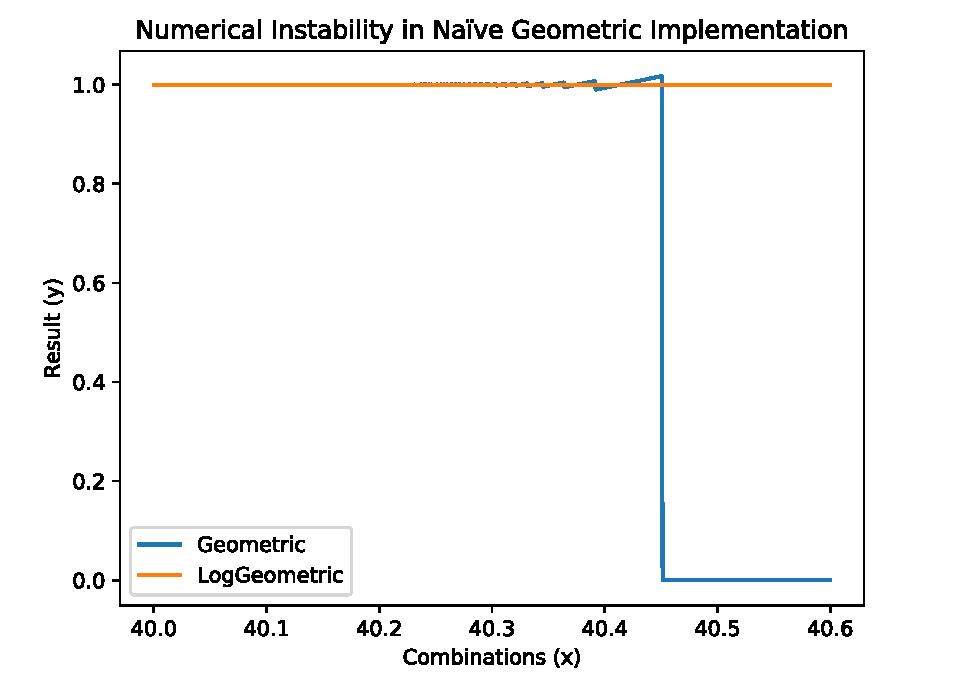
\includegraphics[width=400pt]{figs/instability.pdf}
\caption{Numerical Instability in Naïve Geometric Combination}
\label{fig:num-instab}
\end{figure}

\subsection{Sampling from Distributions}

To sample from probability distributions, a high-quality source of randomness is
needed. After initially investigating the pseudo-random number generators
(PRNGs) in the \texttt{C++11} standard library, I found several other PRNGs that
were shown to be superior in both performance and statistical quality. Of these,
I chose to implement \texttt{xoroshiro128+}, the successor to the well-known
\texttt{xorshift128+} PRNG \cite{vigna2017further}.  As of this writing,
\texttt{xoroshiro128+} has been found to pass more statistical tests than any
other PRNG\footnote{http://xoroshiro.di.unimi.it}. 

The implementation used the publicly-available reference C
code\footnote{http://xoroshiro.di.unimi.it/xoroshiro128plus.c} wrapped in a
\texttt{C++11} \texttt{UniformRandomBitGenerator}, enabling its use as a random
number engine compatible with the \texttt{C++11} \texttt{<random>} library. I
released the implementation as an open source project in case it might be of use
to other \texttt{C++} developers.

Sampling is performed using the \texttt{xoroshiro128+} implementation by
default, but an alternative random source can easily be configured. The PRNG is
seeded using the system's source of randomness, falling back to system time when
this is not available.

\subsection{Early Viewpoints}

The event space for the chorales, determined by our choice of encoding in
Section~\ref{sec:corpus-prep-analysis}, is:
$$ \zeta = [\mathrm{pitch}] \times [\mathrm{onset}] \times [\mathrm{duration}]
\times [\mathrm{keysig}] \times [\mathrm{timesig}]. $$

Recall that the type \emph{onset} specifies the quantised starting time of each
event within a sequence. Using this event space directly when modelling the
chorales with multiple viewpoints is problematic because $[\mathrm{onset}]$ is
not a finite set. In practice, one could ensure its finiteness by fixing a
maximum onset. However, this solution is unsatisfactory, not least because it
bounds the length of possible compositions. Moreover, modelling this type
directly or in combination with other types is not likely to capture any useful
regularity, since it is a global property of each composition.

Instead, define the type \emph{rest} as follows:
$$ \Psi_{\mathrm{rest}}(e_1^k) \triangleq \begin{cases} 
  \Psi_{\mathrm{onset}}(e_1^k) -
  \Psi_{\mathrm{onset}}(e_1^{k-1}) - \Psi_{\mathrm{duration}}(e_1^{k-1}) & k > 1 \\
  \Psi_{\mathrm{onset}}(e_1^1) & \text{otherwise}
\end{cases} $$
and use:
$$ \zeta = [\mathrm{pitch}] \times [\mathrm{duration}] \times [\mathrm{rest}]
\times [\mathrm{keysig}] \times [\mathrm{timesig}] $$
which gives us an entirely local representation, with $[\mathrm{rest}]$ being a
small finite set. The conversion can be performed when the corpus is loaded into
the MVS. 

As suggested by our chosen corpus representation, we make the assumption that
types \emph{keysig} and \emph{timesig} remain constant throughout a single
sequence. Therefore, our task is to predict \emph{pitch}, \emph{duration}, and
\emph{rest} at each timestep. This gives rise to the first implemented
viewpoints: the \emph{basic viewpoints}. These viewpoints simply model these
basic types individually.

\texttt{BasicViewpoint<T>} is simply a wrapper around \texttt{SequenceModel<T>}
that conforms to \texttt{Predictor<ChoraleEvent, T>}. Such viewpoints can be
used to set a baseline performance: a MVS $\set{\mathrm{pitch},
\mathrm{duration}, \mathrm{rest}}$ simply implements a naïve independent
$n$-gram approach.

\subsubsection{Derived Types}

We make use of two abstract interpretations of pitch to improve predictive
performance. The difference in pitch between two consecutive notes, known as the
\emph{sequential interval}, abbreviated to \emph{seqint}, captures regularity
that is invariant to the absolute pitch of notes. Define:
$$ \Psi_{\mathrm{seqint}}(e_1^k) \triangleq \begin{cases}
  \Psi_{\mathrm{pitch}}(e_1^k) - \Psi_{\mathrm{pitch}}(e_1^{k-1}) & k > 1 \\
  \bot & \text{otherwise} 
\end{cases}
$$
to specify the viewpoint \emph{seqint}. The process of lifting a sequence in
$[\mathrm{seqint}]^*$ from a sequence $e_1^k \in \zeta^*$ follows immediately
from this definition. However, the process of reifying a distribution over
\emph{seqint} to give a distribution over \emph{pitch} is less clear.
Algorithm~\ref{alg:reify-seqint} details this process. Note that we need a
context of at least one event so that the absolute pitch of the previous event
is known.

\begin{algorithm}[H]
  \caption{Reification algorithm for \emph{seqint}}
  \label{alg:reify-seqint}
  \begin{algorithmic}[1]
    \Function{reify}{$e_1^k \in \zeta^*$, $p_{\mathrm{seqint}} :
    \mathrm{dist}\langle\mathrm{seqint}\rangle$}
      \State \textbf{assert} $e_1^k \neq ()$
      \Comment might not be able to activate
      \State $p_0 \gets \Psi_{\mathrm{pitch}}(e_1^k)$
      \State $p_{\mathrm{pitch}} \gets \textbf{new}\
      \mathrm{dist}\langle\mathrm{pitch}\rangle$
      \For{$\delta p \in [\mathrm{seqint}]$}
        \State $p' \gets p_0 + \delta p$
        \Comment compute corresponding pitch
        \If{$p' \in [\mathrm{pitch}]$}
          \Comment ensure $p'$ valid pitch
          \State $p_{\mathrm{pitch}}(p') \gets p_{\mathrm{seqint}}(\delta p)$
        \EndIf
      \EndFor
      \State renormalise $p_{\mathrm{pitch}}$ if necessary
      \State \Return $p_{\mathrm{pitch}}$
    \EndFunction
  \end{algorithmic}
\end{algorithm}

It is necessary to check the normalisation of the new distribution, since we may
lose some probability mass from $p_{\mathrm{seqint}}$ in the case that it
predicts an invalid (out-of-range) pitch.

While the interval between two consecutive notes is a salient melodic feature,
another important feature in \emph{tonal} music is the interval with the melodic
\emph{tonal centre}. The tonal centre, a property of the melody's key, is really
a \emph{pitch class} rather than a specific pitch. To account for this this, we
specify a minimum pitch in this pitch class and work modulo $12$.  This
reference pitch is known in the MVS literature as the key's \emph{referent}.

\begin{table}[H]
  \centering
  \begin{tabular}{ r | l | l | l | l | l | l | l | l | l }
    $\Psi_{\mathrm{keysig}}(e_1^k)$ & -4 & -3 & -2 & -1 & 0 & 1 & 2 & 3 & 4 \\
    \hline
    $\Psi_{\mathrm{referent}}(e_1^k)$ & 8 & 3 & 10 & 5 & 0 & 7 & 2 & 9 & 4 
  \end{tabular}
  \caption{Table showing the derivation of \emph{referent} from basic type \emph{keysig}}
  \label{tab:keysig-to-ref}
\end{table}

Using the definition of the \emph{referent} type given by
Table~\ref{tab:keysig-to-ref}, we define the \emph{intref} type:

$$ \Psi_{\mathrm{intref}}(e_1^k) \triangleq 
  (\Psi_{\mathrm{pitch}}(e_1^k) - \Psi_{\mathrm{referent}}(e_1^k))\
  \mathrm{mod}\ 12.
$$

We reify \emph{intref} distributions using Algorithm~\ref{alg:reify-intref}.

\begin{algorithm}[H]
  \caption{Reification algorithm for \emph{intref}}
  \label{alg:reify-intref}
  \begin{algorithmic}[1]
    \Function{reify}{$e_1^k \in \zeta^*$, $p_{\mathrm{intref}} :
    \mathrm{dist}\langle\mathrm{seqint}\rangle$}
      \State \textbf{assert} $e_1^k \neq ()$
      \Comment might not be able to activate
      \State $r \gets \Psi_{\mathrm{ref}}(e_1^k)$
      \State $p_{\mathrm{pitch}} \gets \textbf{new}\
      \mathrm{dist}\langle\mathrm{pitch}\rangle$ 
      \Comment initialise to all zeros
      \For{$i \in [\mathrm{intref}]$}
        \For{$p_0 \in \set{48,60,72}$}
          \State $p' \gets p_0 + r + i$
          \If{$p' \in [\mathrm{pitch}]$}
            \State $p_{\mathrm{pitch}}(p') \gets p_{\mathrm{pitch}}(p') +
            p_{\mathrm{intref}}(i)$
          \EndIf
        \EndFor
      \EndFor
      \State renormalise $p_{\mathrm{pitch}}$ 
      \State \Return $p_{\mathrm{pitch}}$
    \EndFunction
  \end{algorithmic}
\end{algorithm}

Both of these viewpoints were initially implemented as specialised viewpoints
with separate \texttt{IntervalViewpoint} and \texttt{IntrefViewpoint} classes,
both implementing the \texttt{Predictor<ChoraleEvent, ChoralePitch>} interface.

\subsection{Linked Viewpoints}\label{sec:impl-linked-vps}

As discussed previously, pitch and duration are almost never independent,
motivating the implementation of linked viewpoints. I first implemented a
\texttt{BasicLinkedViewpoint} template capable of linking arbitrary \emph{basic
types}, notably enabling a viewpoint linking pitch and duration.

There are a few points to note about the implementation. Recall from
Section~\ref{sec:mvs-formalism} that the formalism treats linked viewpoints as
inherently symmetric objects in that $\tau_1 \otimes \tau_2$ predicts both
$\tau_1$ and $\tau_2$. However, in the implementation, I chose to decouple these
to allow the asymmetric use of linked viewpoints. Use the notation $\tau_1
\rightarrow \tau_2$ to denote the linked viewpoint $\tau_1 \otimes \tau_2$ which
predicts $\tau_2$.

The meta-type \texttt{EventPair<P,Q>} takes viewpoint types $P,Q$ and implements
a viewpoint type $T$ with $[T] = [P] \times [Q]$ following the convention of
Section~\ref{sec:cpp-event-rep} for representing viewpoint types in
\texttt{C++}. The underlying context model for a linked viewpoint over types $P$
and $Q$ is an instance of \texttt{SequenceModel<EventPair<P,Q>>}.

To predict a distribution over either of the linked types, one simply
marginalises the joint distribution: a viewpoint $\tau_1 \rightarrow \tau_2$
predicts a distribution over $[\tau_1] \times [\tau_2]$ and marginalises to
obtain a distribution over $[\tau_2]$.

While the ability to link basic types is useful, it would be better to be able
to link arbitrary combinations of basic and \emph{derived} types. Unfortunately,
the derived types implemented thus far rely on specialised code for lifting and
reification. Implementing $\emph{seqint} \rightarrow \emph{duration}$ would
necessitate a specialised linked viewpoint for this combination of types that
performs the lifting and reification for \emph{seqint}.

\subsection{Generalised Viewpoints}

The insight that led to the development of a fully general viewpoint
implementation was to make the code for \emph{lifting} and \emph{reifying} each
each type a property of the type itself. Additionally, each derived type $\tau$
declares a \texttt{derived\_from} property, which gives the name of the type
from which $\tau$ is derived. 

Template meta-programming was utilised to compute the surface type of any type
\texttt{T} at compile time. The surface type of a type \texttt{T} is
\texttt{T::derived\_from} if \texttt{T} is derived, and \texttt{T} otherwise.

These changes allowed the implementation of \texttt{GeneralViewpoint},
\texttt{GeneralLinkedVP}, and \texttt{TriplyLinkedVP}, all allowing linking of
completely arbitrary types. These template classes perform the appropriate
lifting and reification depending on their inputs.

\begin{table}[H]
  \begin{tabular}{ r | l | p{4.55cm} | p{6.5cm} }
    Type $\tau$ & Predicts & Domain $[\tau]$ & Interpretation \\ \hline
    pitch & pitch & $\set{60,\ldots,82}$ & MIDI pitch of note \\
    duration & duration & $\{$1, 2, 3, 4, 6, 8, 12, 14, 16, 20, 24, 28, 32, 56,
    64$\}$ &
    Duration of note in semiquavers \\
    rest & rest & $\set{0,4,8,12,16,20}$ & Leading rest length in semiquavers \\
    keysig & - & $\set{-4,\ldots,4}$ & Number of sharps in key signature \\
    timesig & - & $\set{12,16}$ & Number of semiquavers in bar \\ \hline
    seqint & pitch & $\set{-12,-9,-8,\ldots,10,12}$ & Sequential melodic interval \\
    intref & pitch & $\set{0,\ldots,11}$ & Harmonic interval with referent \\
    posinbar & - & $\set{0,\ldots,15}$ & Position of event within bar \\
    fib & - & $\set{\texttt{false}, \texttt{true}}$ & \texttt{true} iff.\ event first in bar \\
    fip & - & $\set{\texttt{false}, \texttt{true}}$ & \texttt{true} iff.\ event first in piece \\
    ioi & - & $\{$1, 2, 3, 4, 6, 8, 12, 14, 16, 20, 24$\}$ & Consecutive onset
    difference
  \end{tabular}
  \caption{Complete List of Implemented Types}
  \label{tab:mvs-types}
\end{table}

Table~\ref{tab:mvs-types} shows all implemented types separated into basic and
derived types. All derived types other than \emph{seqint} and \emph{intref} are
non-predictive (cannot be reified). These types are only useful when linked with
a predictive type.

\subsection{Hyperparameter Optimisation}\label{sec:mvs-hyperparams}

Following the architectural constraints of Section~\ref{sec:mvs-arch}, the
free hyperparameters in our model are:
\begin{enumerate}[label=(\arabic*), itemsep=0mm]
  \item The set of viewpoints used. \label{itm:set-vps}
  \item The order $\hbar$ for both the long- and short-term
    model. \label{itm:hbar}
  \item The bias parameters $b_{\mathrm{int}}$ and $b_{\mathrm{ext}}$ for
    distribution combination.
    \label{itm:bias-params}
\end{enumerate}

We can optimise \ref{itm:set-vps} with an automatic viewpoint selection
algorithm: we use a forward stepwise selection algorithm as per Pearce
\cite{pearce2005construction}. For \ref{itm:hbar} and \ref{itm:bias-params} we
use a grid search, illustrated in Figure~\ref{fig:grid-search}. 

Empirically, the resulting surface for \ref{itm:bias-params} is convex for many
values of \ref{itm:hbar}. This supports the argument than we can first optimise
\ref{itm:hbar} and then optimise \ref{itm:bias-params}. However, an important
subtlety is that the setting of \ref{itm:hbar} and \ref{itm:bias-params} can
both potentially affect the set of viewpoints that result from the selection
algorithm.

I used a heuristic approach to choose the hyperparameters, in which we run the
selection algorithm for \ref{itm:set-vps}, optimise \ref{itm:hbar}, then
\ref{itm:bias-params}, and repeat until convergence. While this technique cannot
guarantee to find a global minimum, it is empirically effective.

\begin{figure}[H]
\centering
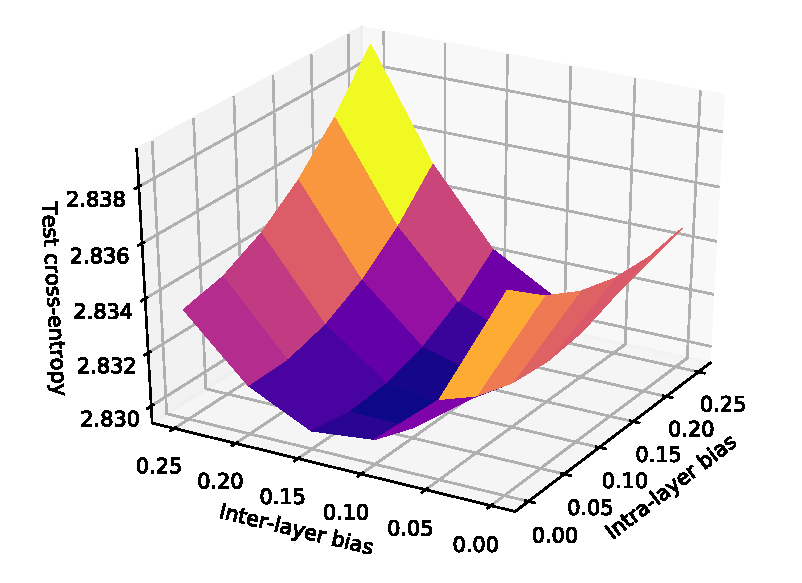
\includegraphics[width=350pt]{figs/bias_plot.pdf}
\caption{Grid search over bias parameters}
\label{fig:grid-search}
\end{figure}

\vspace{4mm}

\subsubsection{Automatic Viewpoint Selection}

A forward stepwise selection algorithm was implemented for choosing a suitable
set of viewpoints from some large pool of candidate viewpoints. This procedure
is detailed in Algorithm~\ref{alg:vp-select}. Along with a pool of viewpoints, a
test set for evaluating the candidate viewpoint systems is required. A parameter
$\epsilon \in \mathbb{R}^+$ controls the minimum margin of improvement necessary
to accept a candidate viewpoint.

\begin{algorithm}[H]
  \caption{Viewpoint selection algorithm}
  \label{alg:vp-select}
  \begin{algorithmic}[1]
    \Function{optimise$\langle\tau\rangle$}{vp-pool, test-set, $\epsilon \in \mathbb{R}^+$}
      \State $S \gets$ \textbf{new}
      stack$\langle$predictor$\langle\tau\rangle\rangle$ 
      \Comment viewpoint stack
      \State $S$.push(basic-vp$\langle\tau\rangle$)
      \State $\mathcal{L}_{\mathrm{prev}} \gets$ evaluate($S$, test-set)
      \Comment baseline loss
      \Loop
        \State $\mathcal{L}_{\mathrm{round}} \gets \infty$
        \For{$V \in$ vp-pool}
          \If {$V \in S$} \textbf{continue}
          \EndIf
          \State $S$.push($V$)
          \State $\mathcal{L} \gets$ evaluate($S$, test-set) 
          \Comment evaluate candidate viewpoint $V$
          \If{$\mathcal{L} < \mathcal{L}_{\mathrm{round}}$}
            \State $\mathcal{L}_{\mathrm{round}} \gets \mathcal{L}$
            \State $V_{\mathrm{round}} \gets V$
          \EndIf
          \State $S$.pop()
        \EndFor
        \If{$\mathcal{L}_{\mathrm{prev}} - \mathcal{L}_{\mathrm{round}} >
        \epsilon$}
          \State $S$.push($V_{\mathrm{round}}$)
          \Comment accept $V_{\mathrm{round}}$, continue
        \Else
          \State \Return $S$
          \Comment no significant improvement, stop
        \EndIf
      \EndLoop
    \EndFunction
  \end{algorithmic}
\end{algorithm}

\section{Recurrent Neural Network}

\subsection{Overview}

A multi-layer LSTM recurrent neural network (RNN) was implemented in Python
using TensorFlow \cite{abadi2016tensorflow}. The network uses \emph{dropout} for
regularisation as per Zaremba et al.\ \cite{zaremba2014recurrent}. A decoupled
``front-end'' to the RNN allows the same internal model to be used for both
language and music modelling. Random walk sampling was implemented for
generation. Furthermore, modifications to the conventional sequence-prediction
RNN architecture were made by feeding the network additional \emph{global}
musical information at each timestep, which was found to improve performance
considerably.

As a precursor to implementing a RNN for music modelling, I implemented a
recurrent network and applied it to the well-studied task of character-level
language modelling. This was done in the hope that the performance of the
network on a well-studied task would be a good indicator of the correctness of
the implementation, as well as to gain an appreciation of the model's
hyperparameters. The results of this are discussed in
Appendix~\ref{apx:rnn-language}.

Since I chose to use TensorFlow to implement the RNN, this necessitated the use
of Python. Unfortunately, because of Python's dynamic type system, many errors
that could be caught at load time are instead caught at runtime. This can lead
to significant time wastage, especially when errors occur following a lengthy
computation. 

To improve on this, I utilised Python 3.6's \emph{type annotations} along with
the static type checker \texttt{mypy}\footnote{http://mypy-lang.org} which was
found to be highly effective at catching problems early and improving the
overall efficiency of Python development.

\subsection{Core Model Implementation}

To guide the discussion of the core RNN implementation, we consider each
hyperparameter in turn and describe the corresponding functionality.

\subsubsection{Model Structure}

Two parameters control the model complexity directly. The number of layers in
the deep RNN is controlled by a parameter \texttt{num\_layers}, and the size of
the LSTM state vectors is governed by \texttt{hidden\_size}.

The LSTM model definition uses the default TensorFlow implementation,
\texttt{BasicLSTMCell}. This class is simply a convenient wrapper around a
handful of TensorFlow graph operations to define an LSTM cell as introduced in
Section~\ref{sec:lstm-prep}. 

\begin{listing}
  \begin{minted}[frame=single, linenos=true, fontsize=\footnotesize,
  mathescape]{python}
lstm_cell = tf.nn.rnn_cell.BasicLSTMCell(hidden_units, state_is_tuple=True)
cells = [lstm_cell] * config.num_layers
self.cell = tf.nn.rnn_cell.MultiRNNCell(cells, state_is_tuple=True)
  \end{minted}
  \caption{LSTM Definition in \texttt{Model} Class}
\end{listing}

The only difference from the LSTM as introduced previously is that the
TensorFlow LSTM implementation adds a bias of $1$ to the forget gate unit. This
prevents forgetting towards the beginning of training, which is useful in
practice.

For simplicity, I chose to unfold the RNN to a fixed size, specified by the
parameter \texttt{seq\_length}. The dimensionality of the mini-batches depends
on a parameter \texttt{batch\_size}.

\subsubsection{Training}

To mitigate the effects of the \emph{exploding gradient problem}, described in
Section~\ref{sec:rnn-train}, I clip the norm of gradients in the network to a
maximum value given by the hyperparameter \texttt{max\_grad\_norm}. This is a
technique utilised by e.g.\ Graves in 2013 \cite{graves2013generating}.

The network is trained by stochastic gradient descent. At train time, the
gradient is computed using each mini-batch in turn to complete an \emph{epoch}
of training (an entire pass through the data). The total number of epochs
performed in a session is given by the \texttt{num\_epochs} parameter.

I chose to implement a learning rate schedule of exponential decay. This enables
large changes in the parameters to be learned towards the start of training and
more fine-grained adjustments to be made towards the end. Specifically, I adapt
the learning rate as:
$$ \alpha_e \gets \epsilon\alpha_{e-1} $$
where $\alpha_e$ is the learning rate at epoch $e$ and $0 < \epsilon < 1$ is a
decay parameter which we call \texttt{lr\_decay}. We fix $\alpha_0$ with a
hyperparameter \texttt{learning\_rate}.

\subsubsection{Regularisation}

After observing significant overfitting with two-layer LSTMs during training,
dropout was applied to the connections between the LSTM layers as per Zaremba et
al.\ \cite{zaremba2014recurrent}.

In the context of the LSTM formulation of Section~\ref{sec:lstm-prep}, we
replace:
$$ \vect{x} = [\vect{h}_{t-1}^l, \vect{h}_t^{l-1}] $$
with
$$ \vect{x} = [\vect{h}_{t-1}^l, \mathrm{D}_p(\vect{h}_t^{l-1})] $$
for equations (\ref{eq:lstm-f}) through (\ref{eq:lstm-d}), where $\mathrm{D}_p$
is the \emph{dropout operator} which randomly sets each component in its result
vector to zero with probability $p$, but otherwise returns its input. 

\subsection{Application to Music}

Unlike the MVS implementation, the RNN uses an opaque representation where each
event in the musical event space is encoded as a natural number: we do not
present the structure of events to the network. However, since the inputs are
first embedded into the RNN's state space with a learned embedding, a suitable
representation can be learned automatically.

\subsubsection{Tonality}

By inspecting the samples produced by early models trained on the base chorale
corpus, an immediate observation was that the output was \emph{tonally
unstable}: compositions would start in a particular key and drift into an
unrelated key. This effect is both jarring to the listener and uncharacteristic
of the target genre.

This stemmed from the fact that the corpus contains compositions in many
different keys. The typical approach taken here is to normalise all of the
compositions by transposing them into a common key.

However, since the MVS could handle training data in many different keys, I
decided to see if the RNN could also do this. To achieve this, I drew
inspiration from a technique used when applying convolutional networks to
optical character recognition (OCR). In OCR, we want to achieve translation
invariance. Furthermore, deep convolutional networks benefit from large amounts
of training data. It is no surprise, then, that artificially translating the
training data can lead to a performance improvement.

To apply this idea to music, observe that, rather than spatial translation
invariance, we want to achieve invariance under musical transposition. Rather
than transposing the training data to a common key, we instead artificially
inflate the training data by transposing each example into many keys (under
certain musical constraints). This was found to eliminate the problem of tonal
instability in the outputs altogether.

\subsubsection{Metrical Stability}

The second major issue exhibited by samples drawn from early RNN models was that
of \emph{metrical instability}: the regular pulse of musical time would be
disrupted at some point in the melody in a way that is audibly jarring and
uncharacteristic of chorale melodies.

\begin{figure}[H]
\centering
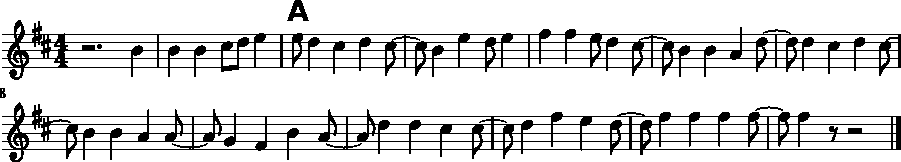
\includegraphics[width=0.9\linewidth]{figs/rnn_likes_syncopation.pdf}
\caption{Poor RNN sample due to metrical disruption}
\label{fig:rnn-instability}
\end{figure}

Figure~\ref{fig:rnn-instability} exhibits this phenomenon with the problem
occurring at position \textbf{A}. Once time is disrupted by this single quaver
beat, the RNN loses track of the musical pulse, and generates notes as if they
were aligned with the bar.

To mitigate this problem, I implement a technique used by Google
Magenta\footnote{https://magenta.tensorflow.org/2016/07/15/lookback-rnn-attention-rnn}
and feed the current \emph{bar position} as an additional input to the network.
This allows the network to act on global metrical information in addition to
local information. This modification was found to largely eliminate this issue.

%\section{Testing and Debugging}
%
%\todo Get lots of points and stickers for demonstrating good software
%engineering practice by testing thoroughly.

\chapter{Evaluation}\label{chap:eval}

The goal of the evaluation is to compare the performance of the two implemented
techniques, the multiple viewpoint system (MVS) and recurrent neural network
(RNN), on the task of generating chorale-like melodies.

The first issue to address is specifying what is meant by \emph{performance}
with respect to melody generation. As with any art form, the success of a music
generation system in the abstract sense is not something that can be specified
objectively. However, one \emph{can} objectively investigate:
\begin{itemize}
  \item The responses of many human participants to subjective evaluation
    criteria in an effort to generalise and draw conclusions about the opinions
    of many more people with respect to such criteria.  
  \item In the case of probabilistic models, such as those implemented, one can
    use objective metrics such as a \emph{cross-entropy} loss function to
    compare the predictive performance of models on unseen data. 

    Under the assumption that the predictive performance of a generative model
    is related to the quality of sampled outputs from the model with respect to
    the chosen subjective evaluation criteria, one can use such metrics as an
    indicator of generative performance. While there are good reasons to make
    this assumption, we do not rely on this metric in isolation.
\end{itemize}

\vspace{4mm}

We start by introducing an objective metric for comparing the \emph{predictive}
performance of the two techniques. Then, we compare the techniques using this
metric, thereby selecting the models to take forward for further evaluation. 

After introducing and justifying subjective evaluation criteria for generated
outputs, we present and discuss an evaluation survey in which participants
listened to model outputs and responded to questions based on the chosen
evaluation criteria. Finally, we conclude by summarising the results of the
evaluation.

\section{Predictive Performance}

In this section we investigate the performance of the models applied to the
problem of \emph{prediction}: the assignment of probabilities to the events in a
sequence. Recall from Section~\ref{sec:gen-models} that both techniques
implemented in this work approximate the joint distribution $p(\vect{x})$ over
sequences $\vect{x} = x_1,\ldots,x_t$ as follows:
$$ p(\vect{x}) = p(x_t | x_{t-1}, \ldots, x_1) p(x_{t-1} | x_{t-2}, \ldots, x_1)
\cdots p(x_1). $$
This allows the process of \emph{predicting} a sequence of length $T$ to be
broken into $T$ steps: for $t = 1$ to $T$, compute $p(x_t | x_{t-1}, \ldots,
x_1)$ where $x_1, \ldots, x_{t-1}$ are the known previous events in the
sequence. 


\subsection{Loss Function}

We use a \emph{cross-entropy} loss function to measure how well a model predicts
a particular sequence, which is derived as follows.  Consider the
$i$\textsuperscript{th} step of prediction. Our model forms a distribution over
possible subsequent events $x'$ in our event space $\zeta$:
$$ p(x' | x_{i-1}, \ldots, x_1). $$
Suppose that we know the ``true'' underlying distribution $q(x' |
x_{i-1}, \ldots, x_1)$. Then the \emph{cross-entropy} between $p$ and
$q$ is given by:
$$ H(p,q) = - \sum_{x' \in \zeta} q(x' | x_{i-1}, \ldots, x_1) \log_2{ p(x' |
x_{i-1}, \ldots, x_1)}. $$
Of course, the underlying distribution $q(x' | x_{i-1}, \ldots, x_1)$ is not
known in practice. However, we can form the \emph{degenerate distribution}
$\widetilde{p}(x' | x_{i-1}, \ldots, x_1)$ which deterministically predicts the
test sequence $\vect{x}$:
$$ \widetilde{p}(x' | x_{i-1}, \ldots, x_1) \triangleq \begin{cases}
  1 & x' = x_i \\
  0 & \text{otherwise}
\end{cases} $$
Then, the cross-entropy of our model predicting $\vect{x}$ at timestep $t$ is
given by: 
$$ H(p,\widetilde{p}) = - \log_2{ p(x_t | x_{t-1}, \ldots, x_1) } $$
giving rise to the cross-entropy sequence loss function
$\mathcal{L}(\vect{x})$
which is the mean cross-entropy for the sequence with respect to our model:
$$ \mathcal{L}(\vect{x}) = - \frac{1}{T} \sum_{t = 1}^T \log_2{ p(x_t | x_{t-1},
\ldots, x_1) }. $$

Given an unseen test set $(\vect{x}_1,\ldots,\vect{x}_N)$, we then calculate the
mean cross-entropy loss:
$$ \frac{1}{N}\sum_{i = 1}^N \mathcal{L}(\vect{x}_i) $$
as a measure of the predictive performance of our model. Since the cross-entropy
at each timestep increases monotonically with $1/p$, it is a direct measure of
the error in our predictions. 

\subsection{Results}

When measuring predictive performance, we are interested in the ability of our
models to \emph{generalise}. For this reason, we must ensure that examples seen
in training do not appear in the test set. In the case of our corpus of melodies
extracted from the chorale harmonisations of J.S.\ Bach, ensuring a hygienic
partition of the data into training and test sets is non-trivial. Since Bach
harmonised melodies multiple times with slight variation in ornamentation and
tonality, the data had to be partitioned based on the underlying melody. To
achieve this, the mapping between chorales and harmonisations\footnote{Taken
from the \emph{Riemenschneider} edition of Bach's chorale harmonisations.} was
encoded by hand in the corpus preparation script.

To compare the techniques, we choose the best-performing model from each based
on the test loss. For the MVS, this was obtained using the hyperparameter
optimisation process of Section~\ref{sec:mvs-hyperparams}, while the RNN
hyperparameters were chosen by careful experimentation. 

With 95\% confidence, the MVS obtained a cross-entropy of $2.826 \pm 0.071\
\mathrm{bits}/\mathrm{event}$ on the test set, while the RNN achieved $3.017 \pm
0.078\ \mathrm{bits}/\mathrm{event}$. Thus, with $95\%$ confidence, the MVS
outperforms the RNN in terms of predictive ability. While this indicates that
the MVS might generate more successful outputs, this remains to be demonstrated.

\subsubsection{Analysis}

\vspace{-4mm}
\begin{figure}[H]
\centering
\subfloat[RNN (mean loss: $3.602\ \mathrm{bits}$)] {
  \label{subfig:rnn-aus-meines}
  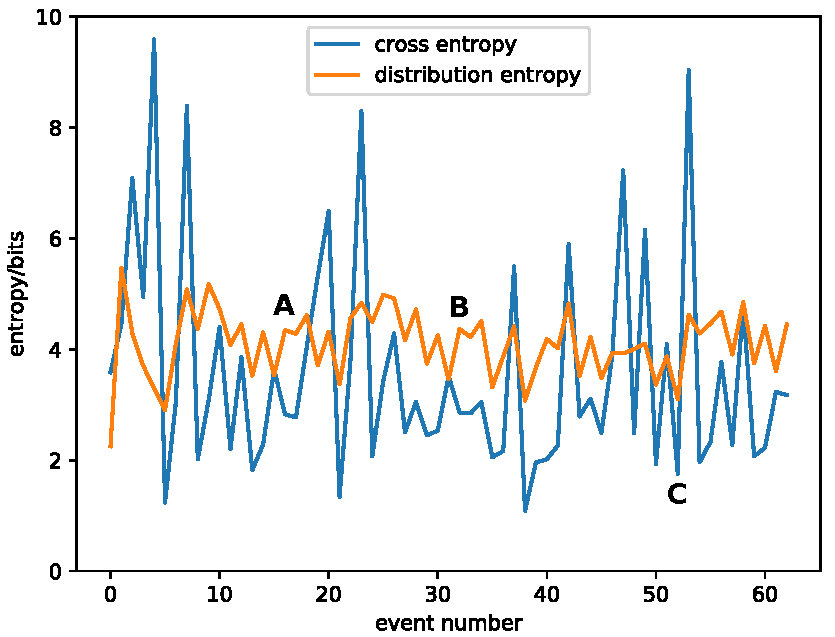
\includegraphics[width=220pt]{figs/rnn_aus_meines_profile.pdf}
}
\subfloat[MVS (mean loss: $3.332\ \mathrm{bits}$)] {
  \label{subfig:mvs-aus-meines}
  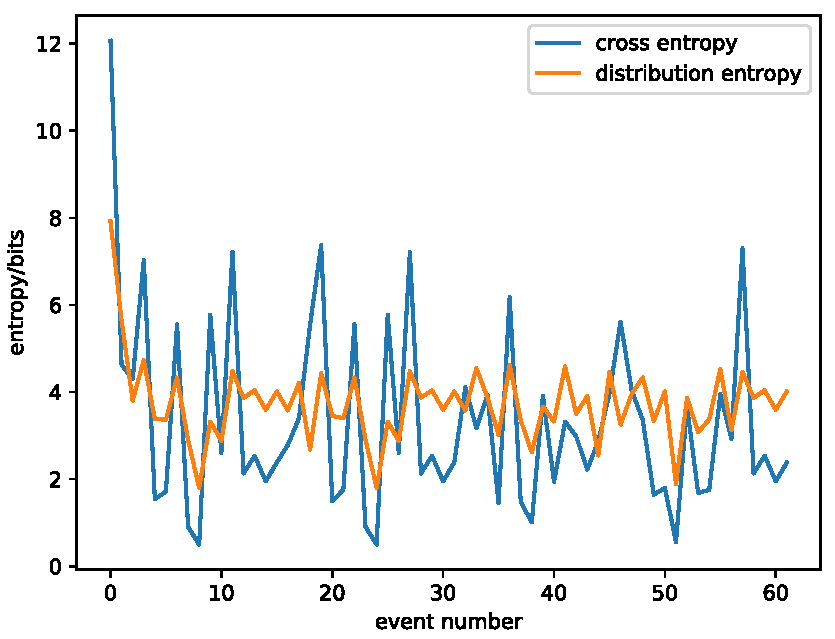
\includegraphics[width=220pt]{figs/mvs_aus_meines_profile.pdf}
}

\subfloat[Input chorale \emph{Aus Meines Herzens Grunde}] {
  \label{subfig:aus-meines-score}
  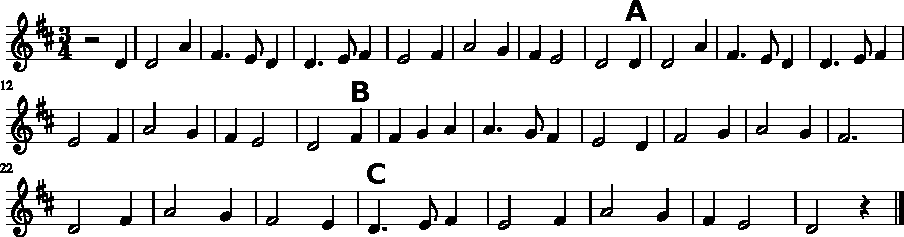
\includegraphics[width=0.8\linewidth]{figs/aus_meines_score.pdf}
}
\caption{Entropy profiles of models predicting representative unseen chorale}
\label{fig:aus-meines-profiles}
\end{figure}

While measuring the overall performance of each model in a single number is
useful, it is not particularly insightful. In this section, we take a more
fine-grained approach by looking at the \emph{entropy profile} of various
sequences with respect to each model. In each profile, we show the
cross-entropy: a measure of how poorly the model predicted each event, and the
distribution entropy: a measure of overall uncertainty in the prediction at each
point.

Figure~\ref{fig:aus-meines-profiles} shows a side-by-side comparison of the two
models on a melody from the test set. At position \textbf{A}, we have direct
re-use of the initial melodic material. At \textbf{B}, we have a related but
distinct middle section, and at \textbf{C}, the opening material returns. It can
be seen that, in this case, the MVS predicts unseen material more successfully
than the RNN, while the RNN predicts re-used material slightly better.

Figure~\ref{fig:danket-dem-profiles} gives an example where the MVS outperforms
the RNN. The note at position \textbf{A} is unexpected by both models, but
several orders of magnitude more so by the RNN. \textbf{B} indicates the start
of the second phrase, and \textbf{C} indicates the return of material from
\textbf{A}. In this case, unlike the RNN, the MVS predicts the re-used material
particularly well. This success might be attributable to the short-term model.

Figure~\ref{fig:als-der-profiles} shows one of the (few) examples where the RNN
outperforms the MVS. Some of the melodies in the corpus, such as this one, are
written with rests between phrases. The positions of the rests in the melody
are given by \textbf{A}, \textbf{B}, and \textbf{C}. It can be seen that the RNN
handles these better, in particular predicting the rest at position \textbf{C}
accurately.

\begin{figure}[H]
\centering
\subfloat[RNN (mean loss: $3.044\ \mathrm{bits}$)] {
  \label{subfig:rnn-danket-dem}
  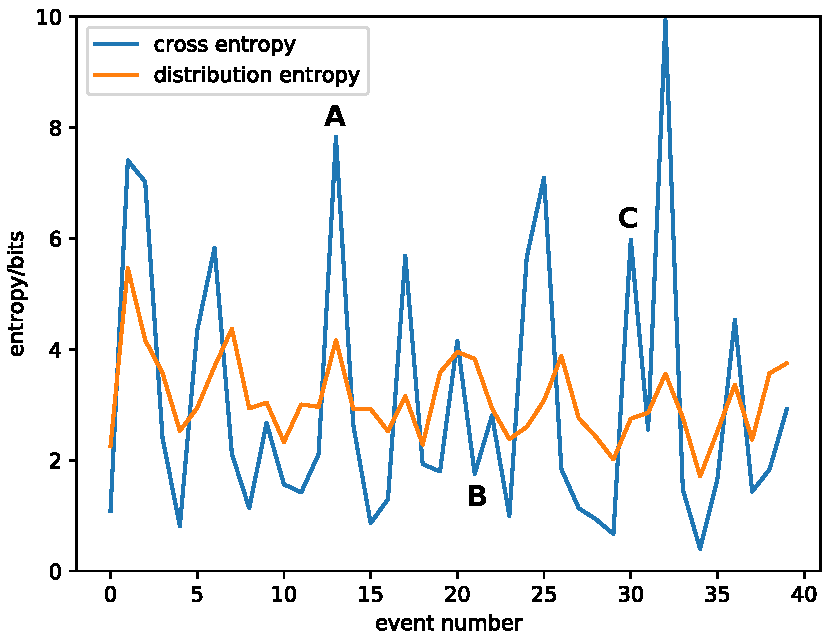
\includegraphics[width=220pt]{figs/rnn_danket_dem_profile.pdf}
}
\subfloat[MVS (mean loss: $1.849\ \mathrm{bits}$)] {
  \label{subfig:mvs-danket-dem}
  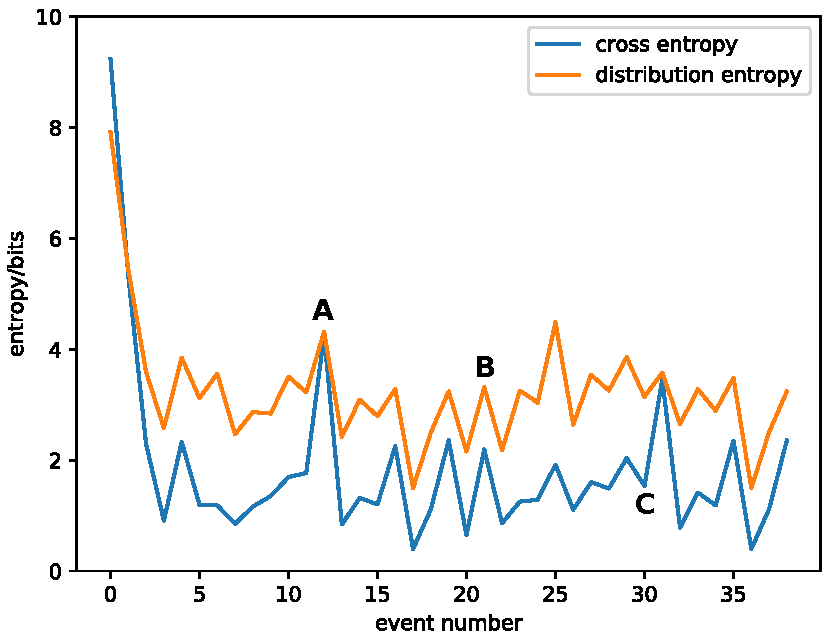
\includegraphics[width=220pt]{figs/mvs_danket_dem_profile.pdf}
}

\subfloat[Input chorale \emph{Danket dem Herrn heut und allzeit}] {
  \label{subfig:danket-dem-score}
  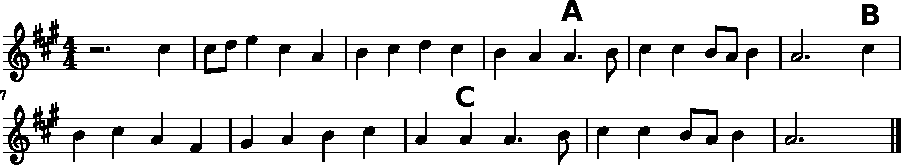
\includegraphics[width=0.85\linewidth]{figs/danket_dem_score.pdf}
}
\caption{Entropy profiles of chorale on which MVS significantly outperforms RNN}
\label{fig:danket-dem-profiles}
\end{figure}

\begin{figure}[H]
\centering
\subfloat[RNN (mean loss: $2.686\ \mathrm{bits}$)] {
  \label{subfig:rnn-als-der}
  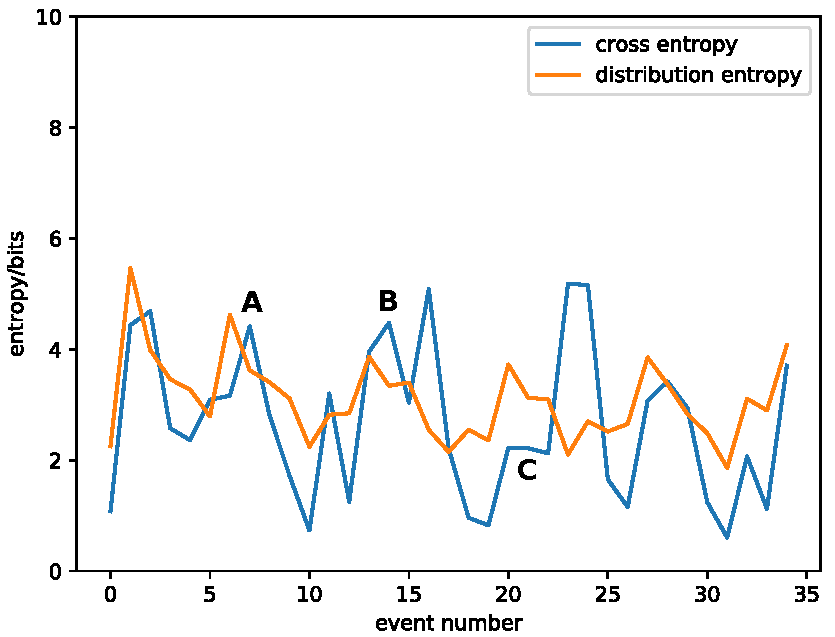
\includegraphics[width=220pt]{figs/rnn_als_der_profile.pdf}
}
\subfloat[MVS (mean loss: $3.031\ \mathrm{bits}$)] {
  \label{subfig:mvs-als-der}
  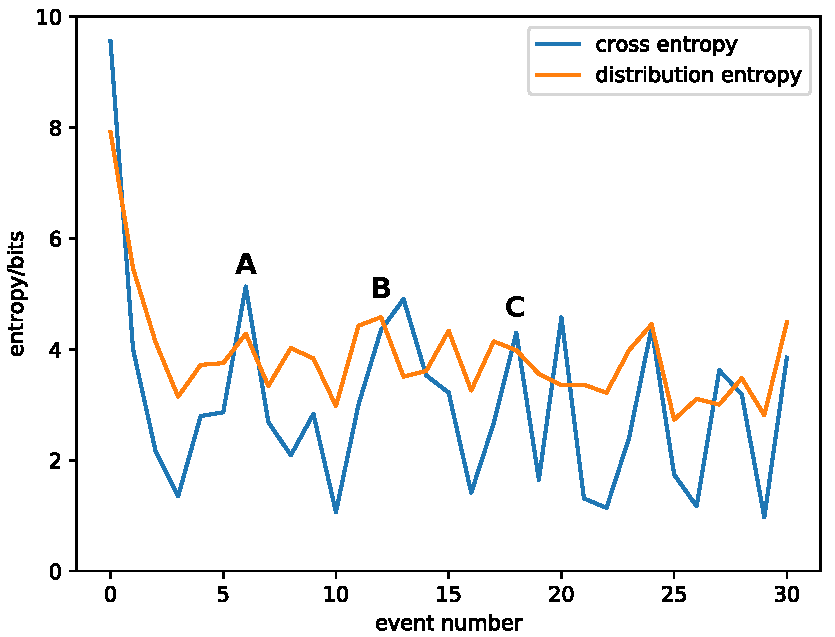
\includegraphics[width=220pt]{figs/mvs_als_der_profile.pdf}
}

\subfloat[Input chorale \emph{Als der gütige Gott vollenden wollt sein Wort}] {
  \label{subfig:als-der-score}
  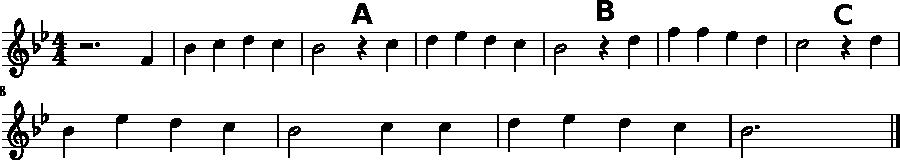
\includegraphics[width=0.85\linewidth]{figs/als_der_full.pdf}
}
\caption{Entropy profiles of chorale on which RNN outperforms MVS}
\label{fig:als-der-profiles}
\end{figure}

We expect our models to reject sequences that are clearly not in the chorale
genre. Models that do not do this may generate undesirable sequences when
sampled. Thus, it is useful to test how our models behave on pathological
inputs. Figure~\ref{fig:path-profiles} illustrates the behaviour of each model
when asked to predict a sequence of thirty identical notes. 

\begin{figure}[H]
\centering
\subfloat[RNN (mean loss: $2.566\ \mathrm{bits}$)] {
  \label{subfig:rnn-path}
  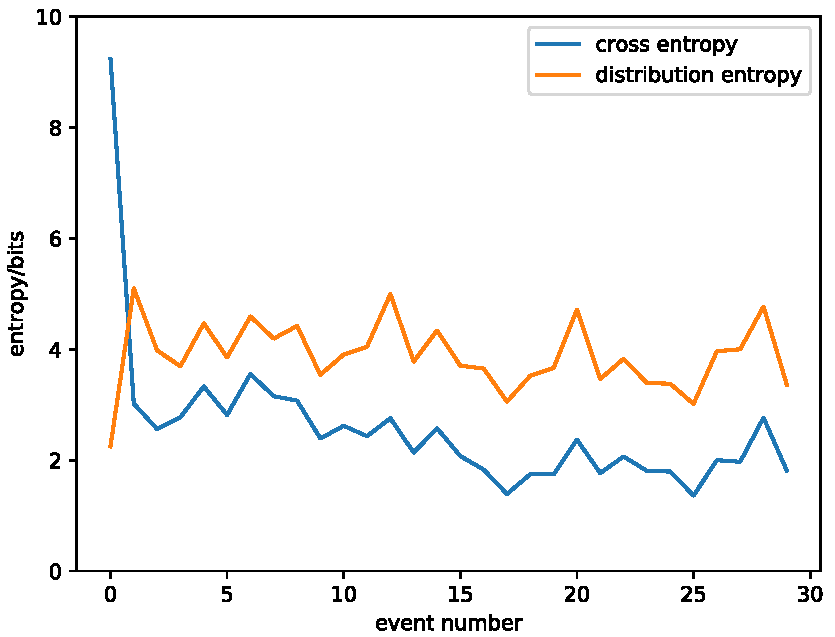
\includegraphics[width=220pt]{figs/rnn_path_profile.pdf}
}
\subfloat[MVS (mean loss: $2.248\ \mathrm{bits}$)] {
  \label{subfig:mvs-path}
  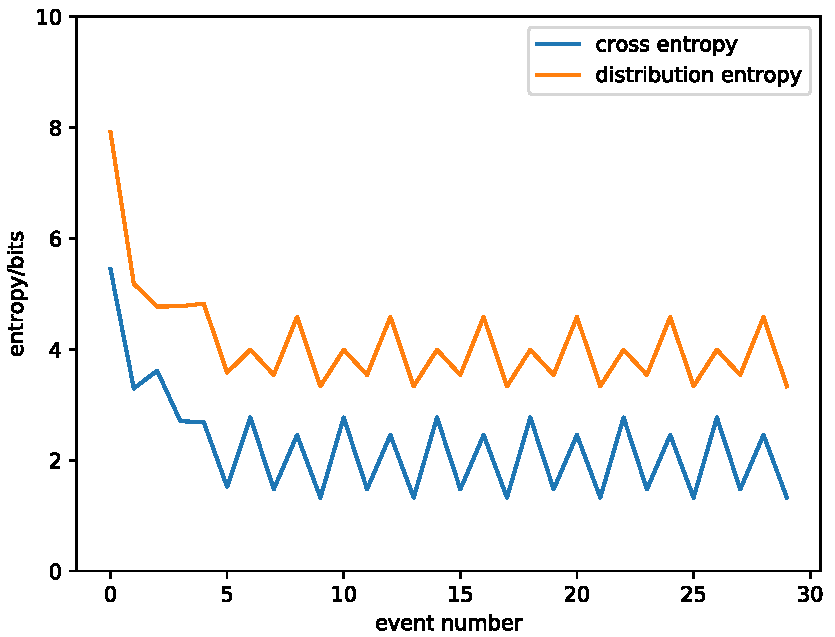
\includegraphics[width=220pt]{figs/mvs_path_profile.pdf}
}

\subfloat[Input Sequence] {
  \label{subfig:path-score}
  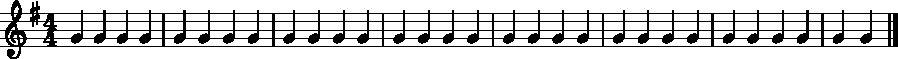
\includegraphics[width=0.85\linewidth]{figs/path_score.pdf}
}
\caption{Entropy profiles of models applied to pathological input}
\label{fig:path-profiles}
\end{figure}

Unfortunately, neither model rejects this input, with both assigning
cross-entropies below their respective losses on the test set. In the MVS, this
is likely due to over-fitting of the short-term model as the sequence is
predicted. The RNN exhibits similar behaviour where the cross-entropy decreases
over time. This is suggestive of an avenue for possible improvements, perhaps
utilising techniques such as \emph{negative training}.

\section{Listening Survey}

\subsection{Evaluation Criteria}

We now turn to the task of evaluating the outputs produced by sampling from the
models. To do this, we need to establish useful \emph{subjective} evaluation
criteria. Since we want our models to imitate a musical style, desirable outputs
should be a \emph{pastiche} of that style. We therefore consider the
\emph{distinguishability} of our outputs from original compositions to be a
primary evaluation criterion of interest.

Secondarily, a desirable property of (arguably) \emph{any} musical composition
is that the composition is perceived as a \emph{unified} and \emph{cohesive}
whole. Often, computer-generated music is \emph{wandering} and lacking
in high-level musical structure. Therefore, we consider the perceived
\emph{coherency} of a musical composition to be a secondary criterion of
interest.

While many other criteria are of interest, we restrict our choice to these two
for the purposes of the listening survey, since the time and concentration
demands on participants should be kept to a minimum.

\subsection{Design and Implementation}

A survey for evaluating samples from the models was implemented in the form of a
web application written using the web framework Ruby on
Rails\footnote{http://rubyonrails.org/}.  The survey stored three pools of
samples: one for the MVS, another for the RNN, and a third for genuine chorale
melodies. Initially, users were asked to give a self-assessment of their musical
ability. Upon a user starting the survey, two samples would be selected from
each pool at random.  After shuffling these samples, they would be presented to
the user, at which point they were asked, for each sample:
\begin{enumerate}[label=\arabic*., itemsep=0mm]
  \item To assess whether the sample was composed by a human (i.e.\ is a genuine
    chorale) or a computer, as well as giving a confidence rating (from 0 to 4,
    expressed with English labels) for this judgement.
  \item To rate, on a Likert scale, the \emph{coherency} of the sample as a
    musical composition.
\end{enumerate}

\begin{figure}[H]
\centering
\subfloat[User self-assessment] {
  \label{subfig:ui-xp}
  
\includegraphics[width=0.8\linewidth]{figs/xp_selection.png}
}

\subfloat[Survey Questions] {
  \label{subfig:ui-survey-qs}
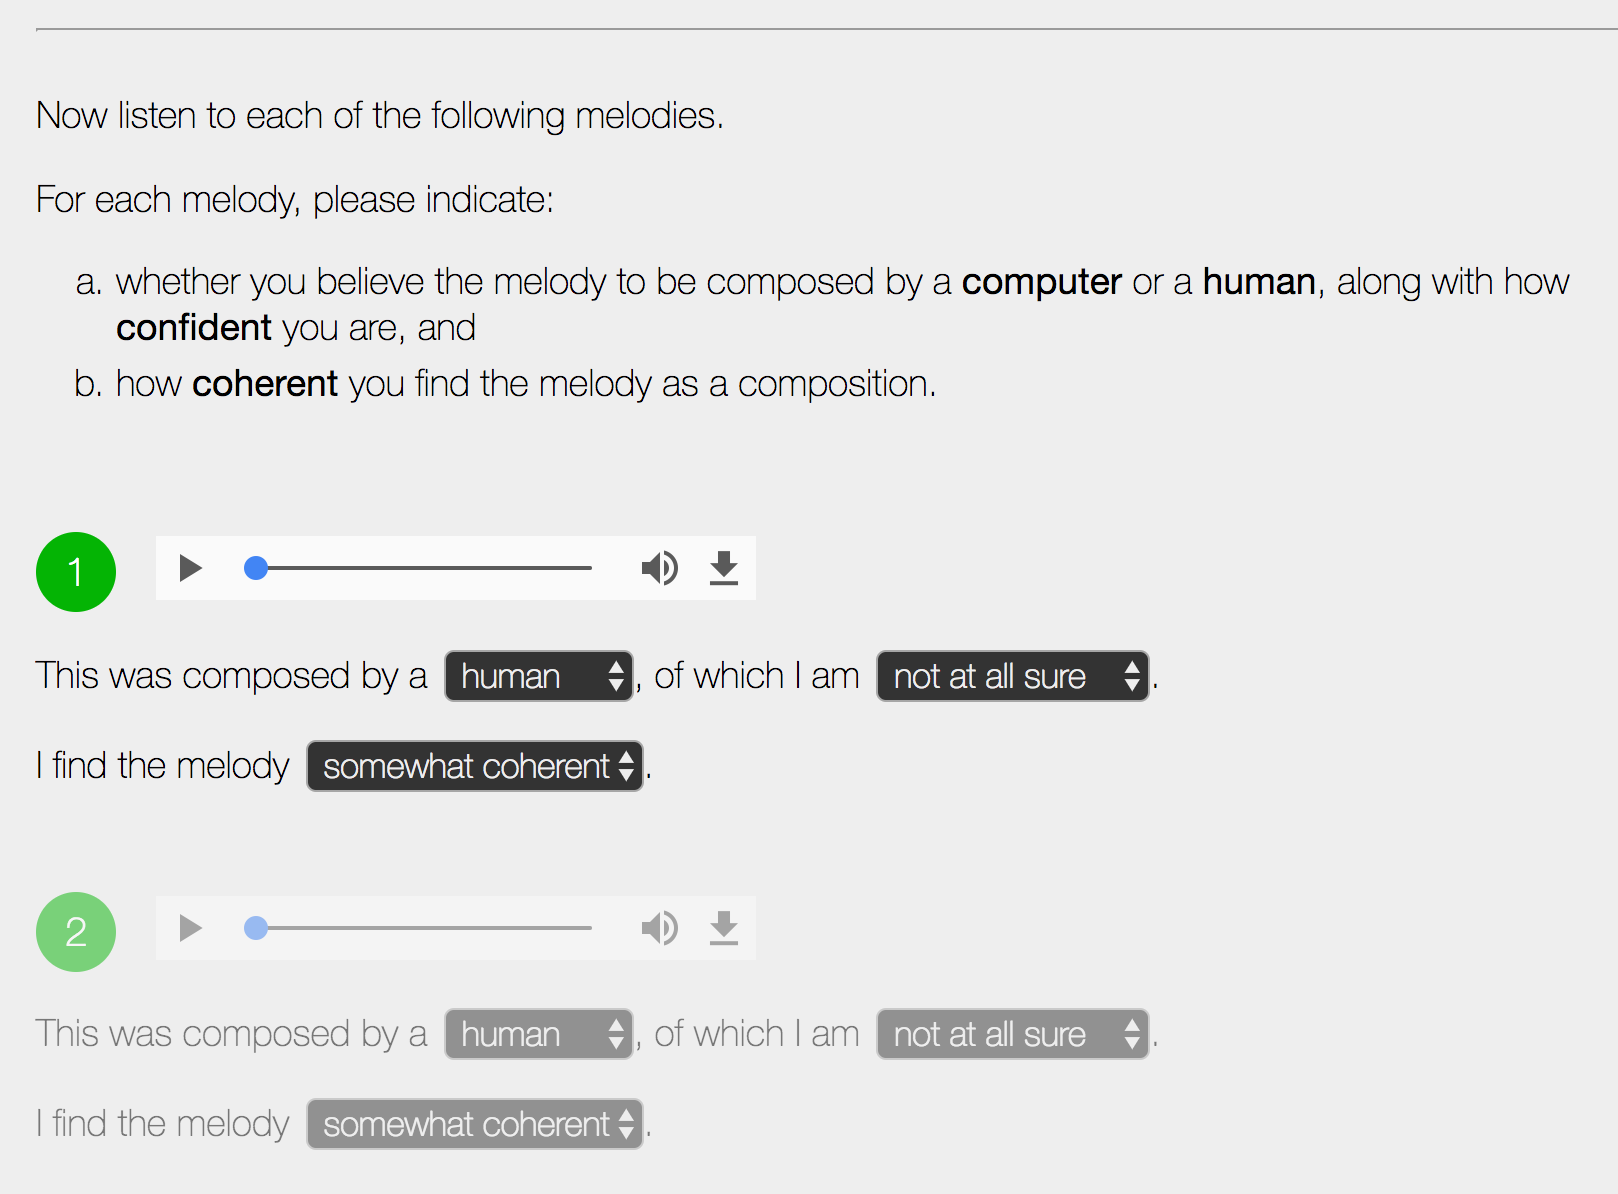
\includegraphics[width=0.8\linewidth]{figs/survey_screenshot.png}
}

\caption{Screenshots of Survey UI}
\label{fig:survey-ui}
\end{figure}

Recent research by Liang et al.\ \cite{liangbachbot} concerning the modelling of
four-part chorales with deep recurrent networks made use of a large-scale
survey-based evaluation. A discussion with one of the authors on possible
improvements to their evaluation led to the use of a user-submitted confidence
metric for classification decisions.

The target demographic of the survey was very broad, making the choice of online
survey appropriate. Due to the use of musical self-assessment, responses from
users across a wide spectrum of abilities were considered useful. Since the
users in the Advanced and Expert groups provide responses of the most value,
links to the survey were distributed to members of various musical groups such
as choirs and music teachers' associations. 

\subsection{Results}

In total, 102 responses were received. The distribution of users' self-assessed
experience levels is given in Figure~\ref{fig:response-dist}.

\begin{figure}[H]
\centering
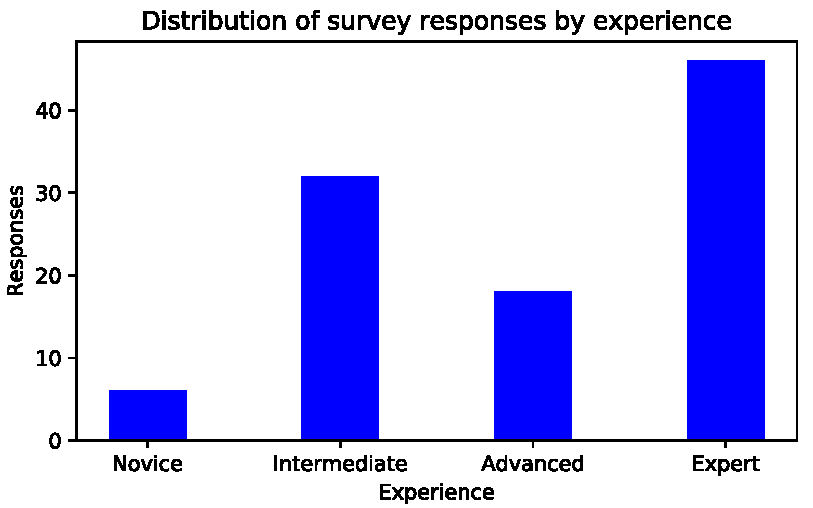
\includegraphics[width=250pt]{figs/response_dist.pdf}
\caption{User experience distribution}
\label{fig:response-dist}
\end{figure}

The primary subjective question asked of the survey participants was whether or
not they believe a sample to be composed by a human or a computer. Each such
classification was recorded along with a user-submitted confidence level on a
scale of 0-4.

Figure~\ref{fig:human-classification} summarises the user classification
results, ignoring the user-submitted confidence metric. All error bars indicate
the standard error from the mean value. We use the classification labels $+1$ to
indicate ``human-composed'' and $-1$ to indicate ``machine-composed''. The line
$y = 0$ in the graphs is therefore the classification performance we expect from
uninformed guessing.

\begin{figure}[H]
\centering
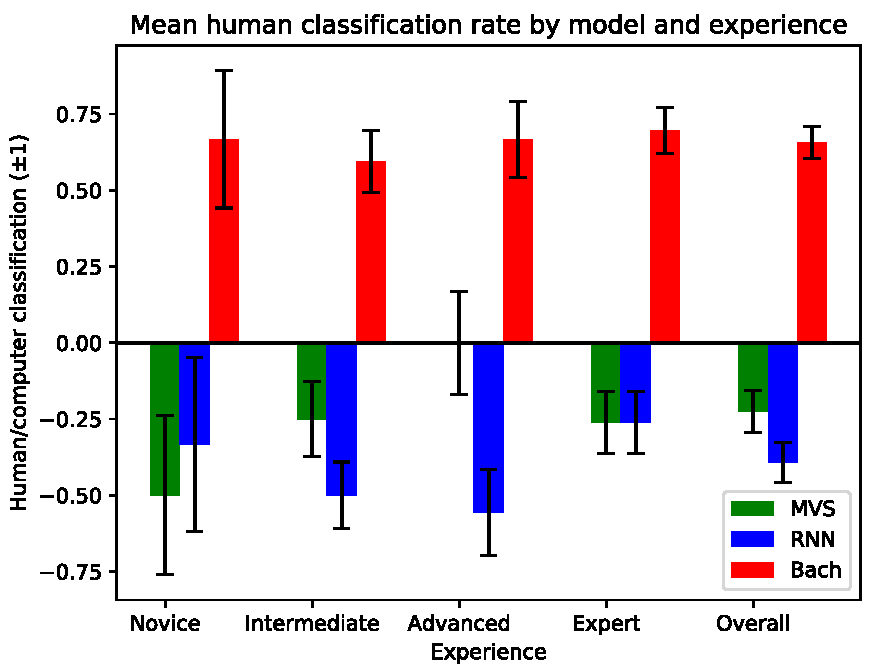
\includegraphics[width=340pt]{figs/human_classification.pdf}
\caption{Human/computer classification}
\label{fig:human-classification}
\end{figure}

Figure~\ref{fig:weighted-classification} takes the user-submitted confidence
metric into account by treating each classification as a vote, and weighting it
by the user's confidence level.
\vspace{2mm}

\begin{figure}[H]
\centering
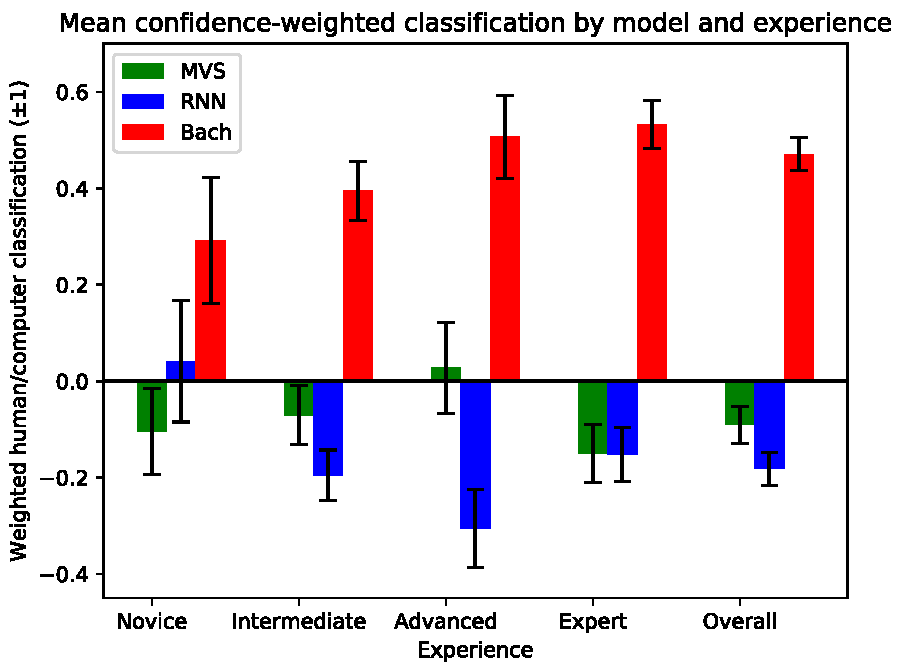
\includegraphics[width=340pt]{figs/weighted_human_classification.pdf}
\caption{Weighted classification}
\label{fig:weighted-classification}
\end{figure}
With only six Novice participants, we consider the volume of data for this class
to be insufficient. Notably, the participants who put themselves in the Advanced
category of users failed to reliably identify the MVS samples as
machine-composed, yet reliably classified the RNN samples as machine-composed.
This is especially pronounced in the confidence-weighted results. These users
also rated the MVS samples as more coherent, as shown in
Figure~\ref{fig:coherency}.

While the classification results for the Expert class are inconclusive, the
coherency ratings might indicate a slight bias towards the RNN, but this is
clearly insignificant. Looking at the aggregate results (labelled `Overall'),
while the coherency ratings are inconclusive, the classification results (both
weighted and unweighted) show that, to within one standard error, users are more
likely to label RNN samples as machine-composed and MVS samples as
human-composed.

\begin{figure}[H]
\centering
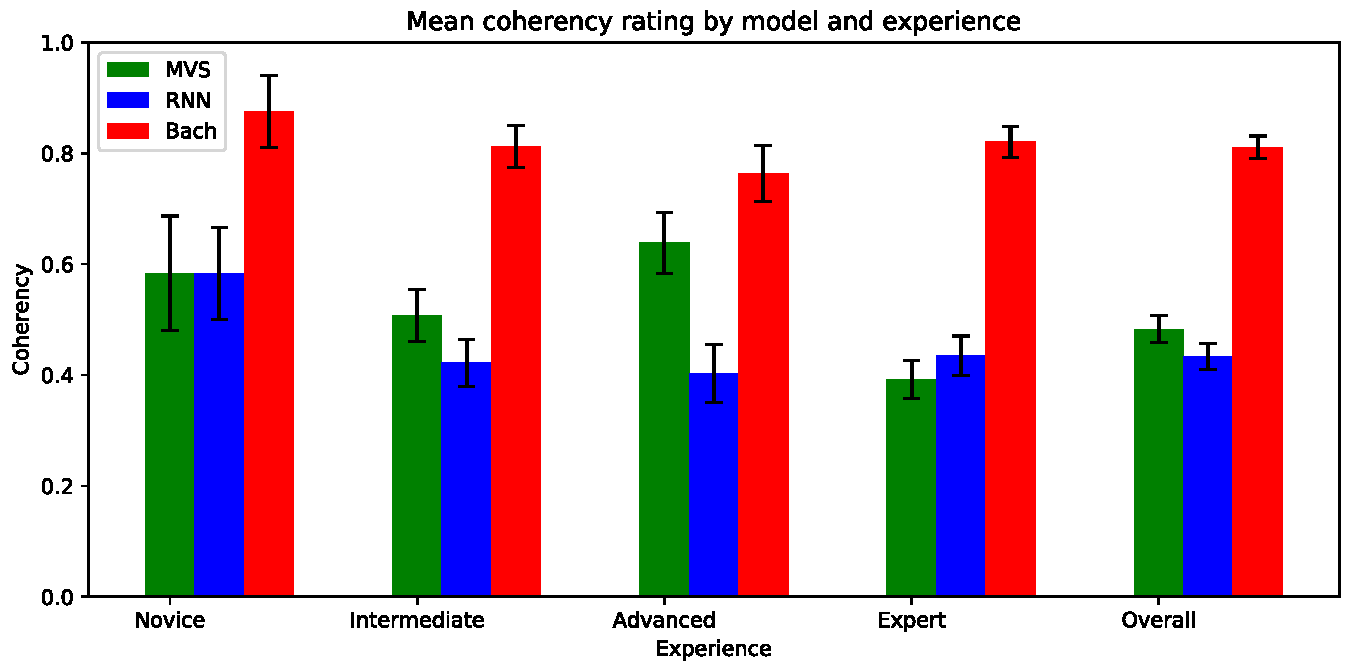
\includegraphics[width=0.75\linewidth]{figs/survey_coherency.pdf}
\caption{Coherency ratings}
\label{fig:coherency}
\end{figure}

%\section{Discussion}
%
%\todo sample analysis x4

\chapter{Conclusion}\label{chap:conc}

\section{Summary}

A multiple viewpoint system (MVS) capable of generating music was implemented.
The implementation provides a general framework for MVS construction and
specialises this framework to the chorale genre. A recurrent neural network
(RNN) for generating music, incorporating domain-specific extensions, was
implemented. Both models meet the success criteria of the project.

The best-performing MVS was found to outperform the best RNN in its ability to
predict unseen chorale melodies. I conjectured that the MVS would therefore
produce more successful musical compositions when sampled. The results from a
listening survey taken by over 100 participants support this hypothesis.  Since
both objective quantitative evaluation of the models and subjective evaluation
of their outputs have been performed, all the success criteria of the project
have been fulfilled. 

These results indicate that the implemented MVS is a superior system for the
generation of melody to the RNN. While we clearly cannot generalise this claim
to all recurrent networks, viewpoint systems, or musical genres, it demonstrates
that a MVS is capable of outperforming models employing sophisticated techniques
from the field of deep learning.

\section{Contributions}

An open source framework for implementing multiple viewpoint systems was
released under the permissive MIT license in the hope to accelerate future work
in this area. 

In this work, we generalised viewpoint combination bias parameters to take on
real values. Empirically, we observed the convexity of the loss surface with
respect to these parameters. Demonstrating this formally and applying techniques
from convex optimisation to eliminate these hyperparameters would be a
possible direction for future work.

\section{Reflection}

There were many choices to be made in refining the project proposal and carrying
out the implementation. In general, my choices of libraries, languages, tools,
and software engineering strategy were all found to be very effective in
accomplishing this. \texttt{C++}, with its flexible and powerful template
system, proved to be an excellent choice for the MVS implementation.
TensorFlow's abstraction of the computational graph was found to be ideal for
the RNN implementation, and the library enabled the expedient development
necessitated by the time-consuming MVS implementation.

A discussion of our results with an expert musicologist revealed that including
\emph{fermata} in our chorale representation might have led to greatly improved
performance of both models, since the models would no longer have to infer
phrase structure. These were initially omitted in the hope of improved
generality.

In hindsight, a more sophisticated PPM variant, such as PPM C or D, might have
led to considerably improved MVS performance \cite{pearce2004combining}. I plan
to extend the open-source implementation with these PPM methods, as well as
implementing the linear-time PPM algorithm proposed in
Section~\ref{subsec:ppm-imp}.

Due to time constraints, the hyperparameters for both models were chosen based
on a single (carefully-chosen) train/test split.  Cross validation would provide
a more robust basis for hyperparameter selection, and should be employed in
future work.

\section{Future Work}

Tools for the automatic generation of lifting and reification code from a
high-level specification would be invaluable for future research on viewpoint
systems. Additionally, applying more recent deep learning methods such as
\emph{recursive} neural networks or \emph{generative adversarial networks} to
music would provide interesting directions for future research.


\section{Closing Remarks}

Our results call into question the contentious issue of whether deep learning
can truly replace feature engineering. In the modelling of music, it is often
desirable to model specific styles, such as the works of a single composer. For
such tasks, the vast quantities of data required to employ deep models are
simply not available. In conclusion, while deep learning has achieved
state-of-the-art results in a number of areas, we should not lose sight of the
effectiveness of specialised models with carefully-engineered features applied
to modest datasets.

%TC:ignore
%%%%%%%%%%%%%%%%%%%%%%%%%%%%%%%%%%%%%%%%%%%%%%%%%%%%%%%%%%%%%%%%%%%%%
% the bibliography
\phantomsection
\printbibliography
\addcontentsline{toc}{chapter}{Bibliography}
%todo Check all the references for typos as Google Scholar certainly has a few!

%%%%%%%%%%%%%%%%%%%%%%%%%%%%%%%%%%%%%%%%%%%%%%%%%%%%%%%%%%%%%%%%%%%%%
% the appendices
\appendix

\chapter{Music Theory}\label{chap:music-theory}

We constrain our discussion to the context of Western classical music, since our
chosen corpus lies within this context. A \emph{pitch} is the musical
abstraction of frequency.  Formally, if $p,q$ are pitches with corresponding
frequencies $\nu_p,\nu_q$, then if $\nu_q = 2\nu_p$, $p$ and $q$ are said to
span an \emph{octave}, with $q$ an octave above $p$. In Western classical music,
each octave is divided into twelve distinct \emph{note names} (A through G
modified by accidentals \insharp{} or \inflat{}, as per
Figure~\ref{fig:keyboard-spn}). A note name, such as `B\inflat' (or,
equivalently, A\insharp), is thought of as not just a single pitch, but a
\emph{pitch class}, the set of all pitches an integer number of octaves above or
below any pitch with that note name.  

\begin{figure}[H]
\centering
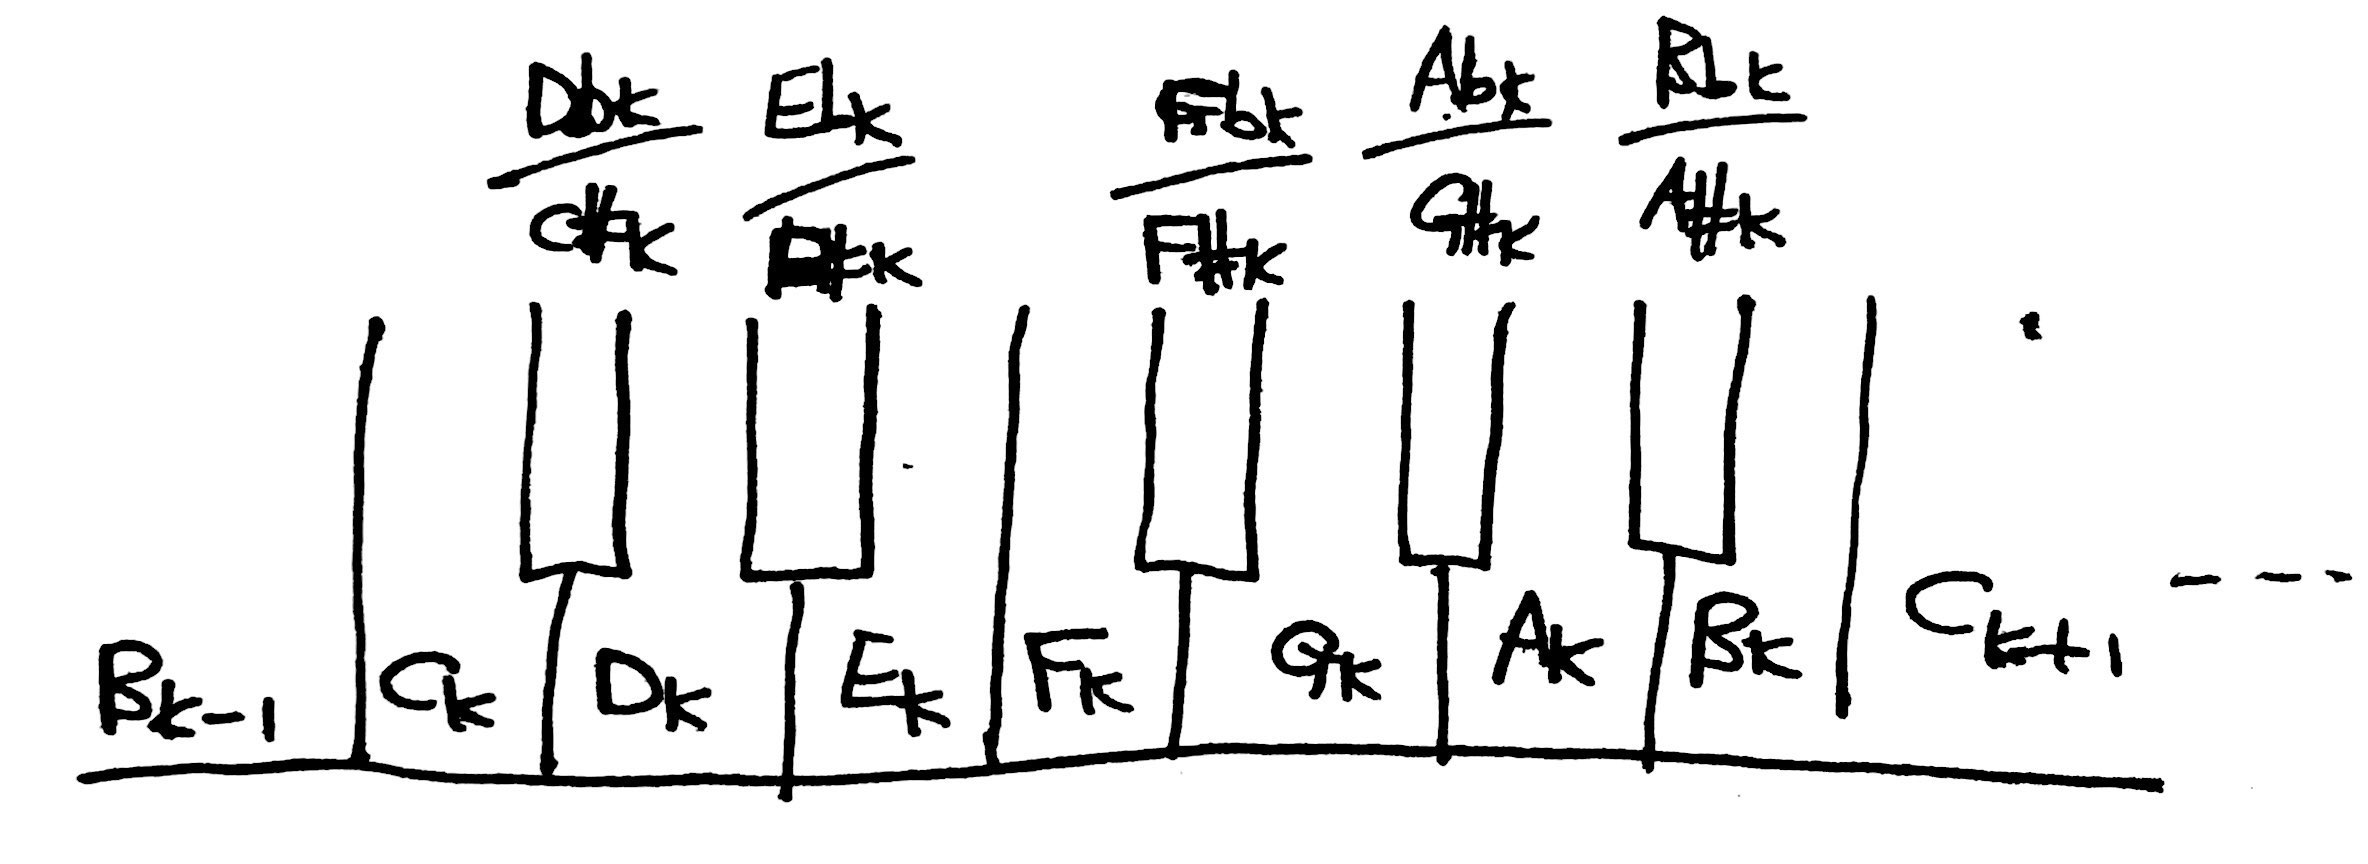
\includegraphics[width=350pt]{figs/piano_spn_tmp.jpg}
\caption{Keyboard showing one octave labelled with SPN note names}
\label{fig:keyboard-spn}
\end{figure}

Formally, given some reference frequency $\nu_N$ for a note name $N$, the set of
frequencies of the pitches in the pitch class for $N$ is given by $\set{ 2^k
\cdot \nu_N\ |\ k \in \mathbb{Z} }.$

The mapping between pitch and frequency is known as \emph{temperament}, which on
modern instruments is typically \emph{equal}, meaning that the frequency space is
equally divided among the twelve pitches in an octave. More precisely, the
$(k+1)$\textsuperscript{th} note of the chromatic scale with base frequency $\nu_0$ is
given by $2^{k/12}\cdot\nu_0$. As an aside, all recordings of
model outputs in this work were made using equal temperament. Herein
we will work with the abstraction of pitch, ignoring the underlying frequencies
of notes.

To refer to specific pitches, we make use of \emph{scientific pitch notation}
(SPN). Write $N_k$ where $N$ is a note name and $k$ is an octave number. To
ground all the definitions made thus far, we use the standard reference
frequency $\mathrm{A}_4 \triangleq 440\ \mathrm{Hz}$.

An \emph{interval} refers to the difference in pitch between two notes.
Consecutive note names are said to be a \emph{semi-tone} apart, and an interval
of two semi-tones is known as a \emph{tone}. Later in this work we shall further
abstract pitch and intervals using MIDI pitch numbering, and further concepts
shall be defined as necessary. In the MIDI tuning standard, $\mathrm{A}_4$
corresponds to pitch number $69$.

Figure~\ref{fig:note-values} shows the musical division of time with the British
English names we shall use to refer to note values. The speed at which a piece
is played can be specified by fixing the number of times any of these note
values occur in one minute.

\begin{figure}[H]
\centering
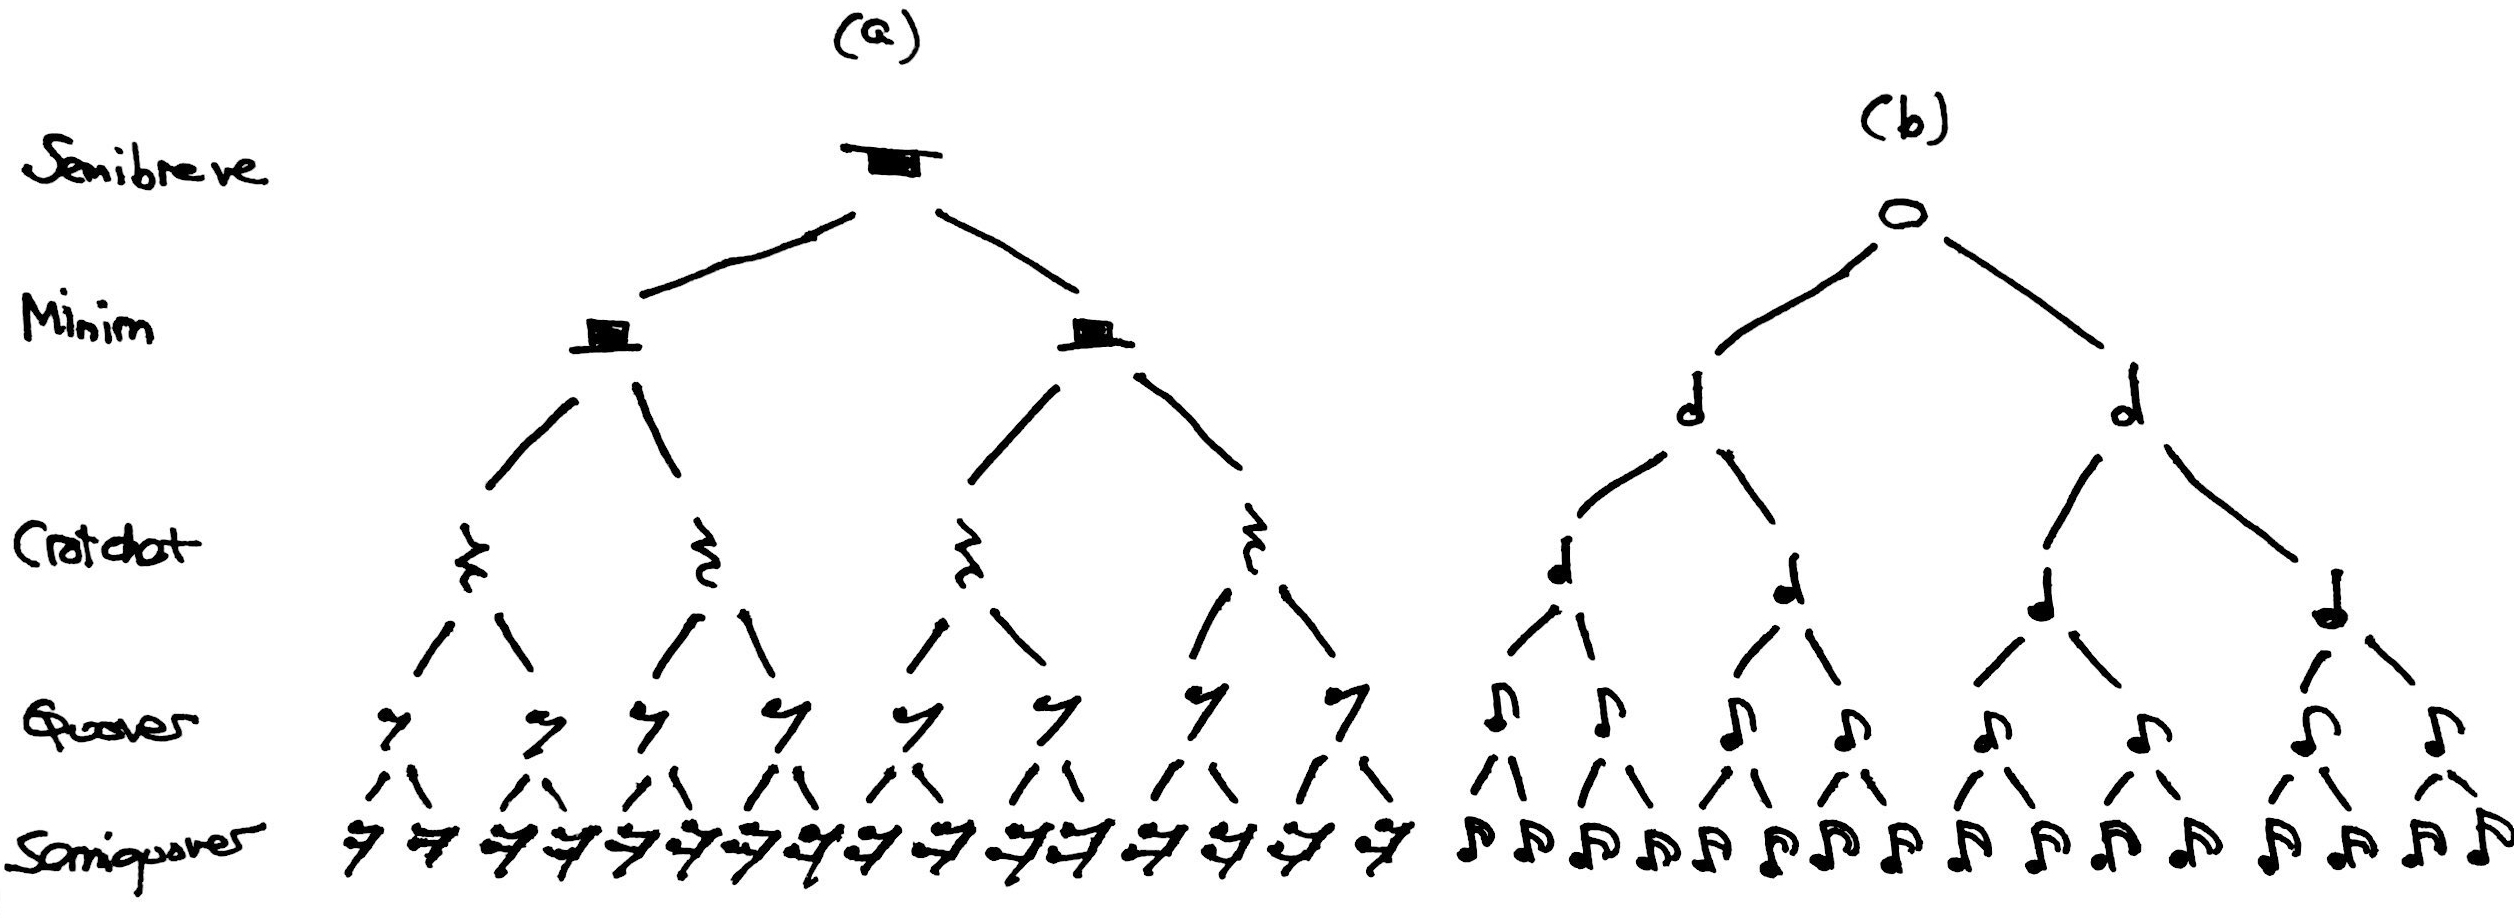
\includegraphics[width=400pt]{figs/note_values_tmp.jpg}
\caption{Notation for Durations of (a) rests and (b) notes}
\label{fig:note-values}
\end{figure}

A dot following a note or rest such as \crotchetDotted{} or \quaverRestDotted{}
indicates that the duration is $1.5$ times the length of its non-dotted
counterpart. Western classical music is typically divided into regular units of
musical time known as \emph{bars}. Both the length of each bar and the regular
rhythmic stress is specified by the \emph{time signature}. The only two time
signatures of concern in this work are \lilyTimeSignature{3}{4} and
\lilyTimeSignature{4}{4}. The numerator indicates the number of \emph{beats} in
a bar, and the denominator the \emph{duration} of each beat. It is important to
be aware that many musical effects are related to the position of a note in the
bar. For example, in \lilyTimeSignature{4}{4}, beats $1$ and $3$ are referred to
as the \emph{strong} beats of the bar and are associated with certain rhythmic
tendencies. We shall exploit this property in the implementation of both
techniques. Figure~\ref{fig:annotated-score} illustrates some of these concepts.

\begin{figure}[H]
\centering
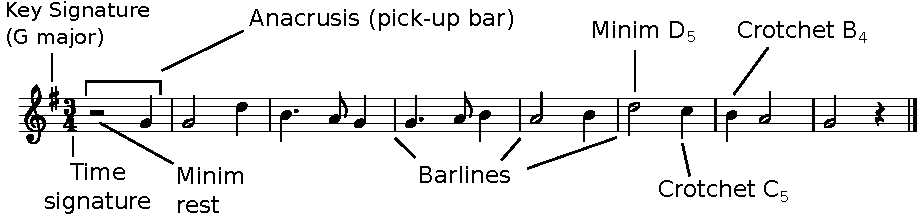
\includegraphics[width=400pt]{figs/aus_meines_annotated.pdf}
\caption{Annotated chorale excerpt illustrating basic music-theoretic concepts}
\label{fig:annotated-score}
\end{figure}

A final concept of importance is that of \emph{tonality}. For our concerns, it
suffices to note that, in \emph{tonal} music (such as the chorales), pitches are
grouped into various \emph{keys}. The note of greatest perceived stability in
this system is known as the \emph{tonic}. 

%%%%%%%% RNN LANUGAGE MODELLING
\chapter{RNN Language Modelling Experiments}\label{apx:rnn-language}

As mentioned earlier, initial experiments were performed on a task of language
modelling. This was done as an indicator of the correctness of the
implementation and to gain an appreciation of the effects of each of the
hyperparameters.

Initial experiments on a dataset of the first ``Harry Potter'' book found raw
predictive performance to increase with the hidden state size for a single-layer
LSTM network.

\begin{verbatim}
epochs: 20, hidden: 32,  lrd: 0.7, loss: 167
epochs: 20, hidden: 64,  lrd: 0.7, loss: 148
epochs: 20, hidden: 128, lrd: 0.7, loss: 134
epochs: 20, hidden: 256, lrd: 0.7, loss: 121
epochs: 20, hidden: 512, lrd: 0.7, loss: 111
\end{verbatim}

Note that, at this point in time, the cross-entropy loss function was
unnormalised, meaning that the loss depended on the length of the unrolled RNN.
I later normalised the loss function to have units of
$\mathrm{bits}/\mathrm{event}$ which enabled direct comparisons between models.

The following is an excerpt of a generated sample from the best-performing of
these single-layer models which demonstrates having learned long-term
dependencies in the form of the high-level structure:

\begin{displayquote}
Come on, how faces repaired his goal ohth, which she felt himself staring up and
down before the squeaking bottom, twitching, on his trunk and a package of
Harry's face.

``Well... for a last few hours - Dumbledore --''

But Malfoy dived it.

``Professor -- Scabbers backed in to my family!''
\end{displayquote}
\vspace{4mm}

\chapter{Project Proposal}
% Note: this file can be compiled on its own, but is also included by
% diss.tex (using the docmute.sty package to ignore the preamble)
\documentclass[12pt,a4paper,twoside]{article}
\usepackage[UKenglish]{isodate}
\usepackage[pdfborder={0 0 0}]{hyperref}
\usepackage[margin=25mm]{geometry}
\usepackage{graphicx}
\usepackage{parskip}
\usepackage{enumitem}
% \usepackage{mathpazo}
% \usepackage{eulervm}
\usepackage{microtype}

\usepackage[style=numeric,backend=bibtex]{biblatex}
\bibliography{refs.bib}

\begin{document}

\cleanlookdateon

\begin{center}
\Large
Computer Science Tripos -- Part II -- Project Proposal\\[4mm]
\LARGE
A Comparison of Statistical Models and Recurrent Neural Networks Applied to the
Generation of Music\\[4mm]

\large
Alex Coplan, St Catharine's College

Originator: Alex Coplan

\today
\end{center}

\vspace{5mm}

\textbf{Project Supervisor:} Matthew Ireland

\textbf{Director of Studies:} Dr S. Taraskin

\textbf{Project Overseers:} Dr M. Fiore \& Dr I. Leslie

% Main document

\section*{Introduction}

The goal of this project is to implement, evaluate, and compare two different
techniques for the algorithmic generation of music. I am particularly interested
in the generation of melody, and ultimately, \emph{polyphony}: multiple
independent melodies interacting with each other in harmonic coherence. In
particular, the two classes of techniques I intend to consider for this project
are:
\begin{itemize}[itemsep=0mm]
	\item Statistical history models such as \emph{multiple viewpoint
			systems} \cite{conklin1995viewpoints}.
	\item Recurrent neural networks.
\end{itemize}

The exact statistical model(s) to be investigated will be determined by the end
of the research phase of the project.

Algorithmic composition is of general interest in computational creativity, but
also has a number of practical applications; one such application being in
\emph{machine-assisted composition}, where a music generation tool aids a human
composer by extending or generating musical ideas. Such tools would be used by a
wide variety of music practitioners.

My intention is to undertake an investigation into the algorithmic composition
of polyphonic music. The first major problem that needs to be tackled in such an
endeavour is that of melody generation. Once this problem has been addressed,
one would subsequently consider the problem ``given a melody (the
\emph{subject}), compose a second (independent) melody (the
\emph{countersubject}) which interacts with, and is coherent with the subject.''
Since the lines in polyphony should be \emph{independent} melodies, it is
necessary to approach the problem of melody generation first.

I therefore propose that the core of the project investigate the application of
these techniques to melody generation. As an optional extension, an
investigation could then be carried out into the composition of two-part
polyphonic music, using these techniques and/or extensions thereof.

I shall follow the approach often taken in the literature of restricting the
domain of source material to stem from a particular musical idiom, e.g.\
\cite{pearce2001evaluation}. This is desirable for a number of reasons, not
least because it introduces a useful evaluation criterion: do the compositions
produced by the system exhibit a coherent musical style, consistent with that
exhibited by the material in the corpus?

In order for this project to be evaluated effectively, in addition to any
information-theoretic or music-theoretic analyses, it is necessary to perform
listening trials on human subjects. Pearce et al.\ \cite{pearce2001evaluation}
outline a framework for evaluation which allows more scientific claims to be
made as a result of the evaluation process. Evaluation would be performed in the
form of a blind trial where the subjects are asked to classify compositions as
human or machine-composed. In this work, it is noted that the participants
exhibited a bias towards classifying compositions as machine composed. This is
something that should be taken into account when designing the evaluation
methodology. An avenue for investigation in this respect is the method of
\emph{three-alternative forced choice}.

Conklin \cite{conklin2003music} notes that random walk is not necessarily the
best method of sampling from a statistical distribution such as that of a
multiple viewpoint system or Markov chain. In this project, I would therefore
also consider exploring different techniques for sampling from statistical
models.
 
\subsection*{Background}

Markov processes are natural statistical models for the analysis of melody, and
are well known as tools for composition \cite{ames1989markov}. Although
effective, Markov processes are far from perfect tools for modelling music.
Specifically, a basic pitch-duration Markov process disregards a considerable
amount of musical information available in the context
\cite{conklin1995viewpoints}.  

However, simply incorporating more musical features into the state space of a
Markov chain leads to an exponential blow-up in space complexity and
necessitates both a large amount of training data for good performance, as well
as solving the sparse data problem (\cite{conklin2003music}, section 2.1).
Moreover, Markov chains do not make use of the long-term context of a system,
which is necessary for modelling the broader sense of sequence and structure
which is present in music.

Conklin et al.\ \cite{conklin1995viewpoints} introduce the method of
\emph{multiple viewpoints} which uses the interpolation of the predictions of
many different context models, each of which considers a different musical
attribute (or some combination of attributes). These include both short-term and
long-term attributes, enabling this method to capture sequence and structure.

It is well known that Recurrent Neural Networks (RNNs) can effectively generate
sequences. RNNs have seen more successful application in music following the
introduction of long short-term memory (LSTM) techniques \cite{eck2002lstm}.
Without use of LSTM, RNNs exhibit similar problems to Markov chains in that the
output does not contain the elements of sequence and structure that one might
expect from compositions in the corpus.

\section*{Starting point}

In Lent term of 2016, I gave a talk (as part of Churchill college's Computer
Science talk series) on melody generation using Markov chains. I also
constructed a demo in Ruby which implemented a parser for ABC
notation\footnote{\url{http://abcnotation.com/}} along with a simple Markov
chain model, trained of a small corpus of hymn tunes, which generated tunes by
random walk. 

Although this experience led me to this choice of project, the implementation of
a model such as a multiple viewpoint system is considerably more involved, and
the architecture vastly different. The implementation of this model will
therefore be carried out from scratch.  The neural network will be implemented
using a library such as Google's
TensorFlow\footnote{\url{https://www.tensorflow.org/}}.

As an organ scholar (and previously an A-Level music student), I have
considerable experience with performing polyphonic music (and some experience of
analysis), especially that of the renaissance and baroque eras. I believe this
domain knowledge will prove especially useful for making musically-informed
decisions in this project. 

\section*{Resources required}

For this project I shall primarily use my own laptop. Backup will be primarily
in the form of a GitHub-hosted repository, but I will also perform backups of
the project files to an external hard drive as well as multiple cloud providers
(Google, Apple, Dropbox) and the MCS. Should my main computer suddenly fail, I
can easily continue the project using MCS computers by cloning the code from the
GitHub repository.

Although datasets can easily be compiled from online sources, it may also be of
use to have a MIDI keyboard to be able to input arbitrary musical data. I own a
MIDI keyboard which would be suitable for these purposes. I will make use of
open-source software (such as MuseScore\footnote{\url{https://musescore.org/}})
for synthesis of MIDI and other musical data. I require no other special
resources.

\section*{Work to be done}

I will employ an agile software development methodology when undertaking this
project. The ordered list of sub-tasks within this project are:
\begin{enumerate}

\item Devising and implementing an internal representation of musical data,
	along with a simple ``music theory engine'' to process this data.  

\item Implementing a simple parser for some form of input notation (ABC, MIDI,
	MusicXML); the exact form to be determined in the research phase.  

\item Implementing and iteratively refining the statistical model (e.g. multiple
	viewpoint system).

\item Implementing and iteratively refining the RNN for melody generation.  

\item Designing and carrying out a scheme for human evaluation.

\item Making iterative improvements to the two models.

\end{enumerate}

\section*{Success criteria}

\subsection*{Core Tasks}

The project will be a success if I have:
\begin{itemize}
	\item Successfully implemented a statistical model such as a multiple
		viewpoint system capable of generating melody.
	\item Successfully implemented a technique based on recurrent neural
		networks capable of generating melody.
	\item Performed an evaluation and comparison of the two
		models, answering questions such as:
	\begin{itemize}
		\item Can human subjects distinguish the machine-composed output
			from the human-composed samples in the corpus?
		\item Do human subjects classify the machine-composed output as
			adhering to the specified style?
	\end{itemize}

	Note that the success of the evaluation stage is not predicated on the
	answers to the questions given above, but merely whether the evaluation
	is conducted in a scientific manner.
\end{itemize}

\subsection*{Extension Tasks}

The project will be judged as a success if all the core tasks have been
completed. The extension tasks won't be used to judge the success of the
project, but it will have gone above and beyond expectations if one of them is
completed.

These possible extensions include:
\begin{itemize}
	\item Extending a multiple viewpoint system to generate polyphony.
	\item Extending a RNN to generate polyphony.
	\item Exploring extensions and adaptations of multiple viewpoint
		systems.
\end{itemize}

\section*{Timetable}

Planned starting date is 16/10/2011.

\begin{tabular}{ p{4cm} | p{11cm} } \hline 
% TODO: 2 week blocks, start earlier to include proposal week.
% TODO: 2-page spread

16/10/16 - 27/10/16 Mich. Weeks 2-4 & \textbf{Research phase}.
Research multiple viewpoint systems, RNNs, and evaluation techniques.
Investigate options for corpus material and format. This will inform the type of
parser that should subsequently be implemented. Devise and fix an internal
representation for musical data. Design specific multiple viewpoint system based
on \cite{whorley2013phd}. The corpus should also be prepared as fully as
possible during this stage. Familiarisation with libraries (e.g. TensorFlow)
should be accomplished during this phase.

\textbf{Milestone}: Report summarising research handed to supervisor.
\\ \hline
03/11/16 - 10/11/16 \newline Mich. Week 5 & \textbf{Preliminary Implementation}. 
Implement parser for chosen corpus format. Implement internal representation as
determined in the previous phase. Write test suite for the above. 
\\ \hline
10/11/16 - 30/11/16 \newline Mich. Weeks 6-8 & \textbf{MVS Implementation I}.
First iteration of multiple viewpoint system to be completed in these three
weeks. System need not be complete in terms of the exact viewpoints used.
However, the underlying machinery should be. In particular, context models,
viewpoint representation, prediction interpolation etc. should all be
implemented, such that a MVS can be constructed, trained, and used for
generation.
\\ \hline
01/12/16 - 22/12/16 \newline Christmas Vac. Weeks 1-3 & \textbf{RNN Implementation I}.
Implement LSTM Recurrent Neural Network. 
\\ \hline
29/12/16 - 12/01/17 \newline Christmas Vac. Weeks 4-5 & \textbf{MVS Implementation II}.
Implement full multiple viewpoint system. Investigate different choices of
viewpoints as per the R\&D outlined in the research phase. 
\\ \hline
12/01/17 - 26/01/17 \newline Lent Week 0 & \textbf{RNN Implementation II}.
Finish RNN implementation. Train network on entire corpus.
\\ \hline

\end{tabular}

\printbibliography

\end{document}


%TC:endignore

\end{document}
